\documentclass{article}
\usepackage{naturetex}
\usepackage{booktabs}
\usepackage{multicol}
\usepackage{multirow}
\usepackage{amsmath}
\usepackage[mathlines]{lineno}
\setlength\linenumbersep{12pt}
\renewcommand\linenumberfont{\normalfont\footnotesize}
\renewcommand{\baselinestretch}{1.5}
\usepackage{amssymb}
\usepackage{algorithm}
\usepackage[noend]{algpseudocode}
\usepackage{setspace}
\usepackage{caption}
\usepackage{threeparttable}
\usepackage{pdflscape}
\usepackage{array}
% \captionsetup[algorithm]{skip=14pt}

\renewcommand{\baselinestretch}{1.5}
\newcolumntype{C}[1]{>{\centering\arraybackslash}p{#1}}

\newcommand{\name}{Frogent }
\newcommand{\nam}{Frogent}
\newcommand{\oa}{Orchestrate agent}
\newcommand{\ra}{Retrieve agent}
\newcommand{\fa}{Forge agent}
\newcommand{\ga}{Gauge agent}
\newcommand{\keywords}[1]{\textbf{Keywords:} #1}

\begin{document}
\linenumbers
\maketitle

{\setstretch{1.0}
% *** ABSTRACT ***
\section*{Abstract}
Computational drug discovery offers models for target analysis, molecular generation, structural assessment, and synthesis planning, yet these capabilities remain difficult to combine into a coherent decision process. We introduce FROGENT, a multi-agent framework that coordinates evidence retrieval, molecular and peptide design, evaluation, and retrosynthetic planning through shared context and typed tools. FROGENT uses pretrained models without task-specific parameter training; specialization arises from role instructions, evidence control, and tool-mediated execution. Across eight tasks and matched base-model studies, the framework improved evidence-grounded performance across diverse language models, enabled reliable structured target and drug retrieval, and used evaluation feedback to redirect molecular-generation effort. Comparisons with adaptations of related agent systems show complementary strengths across property, screening, design, and retrieval tasks. FROGENT thereby establishes evidence-controlled orchestration as a practical route for connecting heterogeneous computational drug-discovery resources while retaining transparent uncertainty and human scientific oversight.

\keywords{Drug Design, Multi-Agent System, Large Language Model, Model Context Protocol.}
}

\section*{Introduction}
Traditional drug development is a capital-intensive and time-intensive endeavor, frequently requiring more than a decade and multi-billion-dollar investments to deliver a single therapeutic to market. Recent advances in artificial intelligence (AI) are catalyzing a paradigm shift in pharmaceutical research by enabling data-driven, scalable, and more efficient discovery strategies \cite{sadybekov2023computational}. AI-driven methodologies are now being systematically integrated across the drug discovery pipeline, encompassing target identification \cite{pun2023ai}, de novo molecular design \cite{zhang2024deep}, and toxicity and safety assessment \cite{wilde2024implementation}. Despite substantial gains in accuracy and cost-effectiveness, the AI ecosystem for drug discovery remains fragmented. Most existing approaches are realized as isolated web services, standalone software, or task-specific code modules, each addressing discrete stages of the pipeline rather than an integrated, end-to-end workflow \cite{zhang2025artificial}. This lack of interoperability and end-to-end automation constrains both operational efficiency and the holistic evaluation of drug candidates.

Fortunately, the rapid evolution of large language models (LLMs), including GPT4 \cite{achiam2023gpt}, Qwen3 \cite{yang2025qwen3}, and DeepSeek-R1 \cite{guo2025deepseek}, has demonstrated strong capabilities in reasoning, planning, decision-making, and tool-augmented action execution within interactive environments. Consequently, LLM-based agents are particularly well suited to addressing complex, multi-step drug design problems, as they can operate effectively in structured scientific settings, support long-horizon reasoning and planning, and systematically decompose the drug discovery process into interdependent subtasks \cite{gao2024empowering}. Moreover, LLM-based multi-agent systems provide a principled paradigm for drug design by harnessing collective intelligence while preserving the functional specialization of individual agents, coordinating communication and collaboration among multiple domain-specific agents. Such systems can integrate heterogeneous expertise and orchestrate tool-augmented workflows, thereby enabling more efficient and autonomous end-to-end drug design \cite{zhao2025llm}.

Considerable efforts have been devoted to the development of AI agents for drug design and discovery. Representative systems span multiple stages of the pipeline. For target discovery, OriGene is a self-evolving multi-agent system that functions as a virtual disease biologist, enabling the systematic identification of mechanistically grounded therapeutic targets \cite{zhang2025origene}. In drug–target interaction modeling, DrugAgent introduces an automated programming framework in which an LLM-based planner generates and refines solution strategies while an instructor module integrates domain knowledge \cite{liu2024drugagent}, and DrugMCTS synergistically combines retrieval-augmented generation, multi-agent collaboration, and Monte Carlo tree search for drug repositioning \cite{yang2025drugmcts}. For lead identification and optimization, ChatDrug integrates prompting, retrieval, domain feedback, and conversational modules to streamline molecular editing tasks \cite{liu2024conversational}. Beyond in silico design, VirtualLab formulates an LLM-based principal investigator agent that collaborates with human researchers to design SARS-CoV-2 nanobodies \cite{swanson2025virtual}. In the context of chemical synthesis, LLM-RDF employs six specialized LLM-based agents to guide the end-to-end synthesis development process \cite{ruan2024automatic}, while ChemCrow combines chain-of-thought reasoning with expert-curated chemistry tools to automate organic catalyst synthesis \cite{m2024augmenting}. Nevertheless, most existing agent-based systems are confined to specific stages of the drug design pipeline, thus remain at the level of module-level intelligence augmentation, rather than constituting end-to-end drug design systems. Although DrugPilot \cite{li2025drugpilot} and PharmAgents \cite{gao2025pharmagents} aim to streamline and automate the pharmaceutical research pipeline, they rely on predefined workflows or manually specified agent roles, resulting in largely fixed execution paths that limit the effective exploitation of LLMs’ knowledge-driven reasoning, long-horizon planning, and intermediate reflection capabilities required for truly autonomous, end-to-end drug discovery workflows.

To address these challenges, we introduce \name, a \textbf{f}ull-p\textbf{ro}cess dru\textbf{g} d\textbf{e}sign multi-age\textbf{nt} system that enables end-to-end coordination of computational drug-discovery workflows. By explicitly modeling reasoning and planning, \name supports long-horizon, multi-step decision-making, thereby leveraging the cognitive capabilities of large language models. In addition, \name adopts a deeply integrated multi-agent collaboration framework that enforces goal alignment, facilitates information sharing, and coordinates strategy optimization across agents. Through the integration of language-based interaction with adaptive orchestration, \name lowers technical barriers and streamlines decision-making across the pipeline. It is designed to support problem formulation, objective specification, molecular design, and systematic evaluation across small-molecule and peptide workflows. We evaluate \name through eight drug-discovery task categories and three representative case studies. The revised analysis reports task-specific performance, component contributions, and provider limitations, defining the demonstrated scope of the integrated framework while retaining human oversight for scientific interpretation and campaign-level decisions.



% *** RESULTS ***
\section*{Results}

\subsection*{Architecture Design of Frogent}
To systematically address the complexity of the end-to-end drug discovery process, we architected \name as a decentralized, collaborative multi-agent system. This design paradigm moves beyond a monolithic agent, embracing a division of labor that assigns distinct responsibilities to specialized agents, as illustrated in Figure \ref{fig:Architecture}. The framework is composed of four cornerstone agents: \oa, \ra, \fa \ and \ga. Upon receiving a user's high-level goal, the \oa, serving as the central controller, initiates the workflow by performing planning: it decomposes the goal into a structured task graph of executable subtasks and dispatches them to the appropriate specialized agents. A central feature is the Global Context, a dynamic memory module managed by the \oa, which maintains the state of the entire workflow. This context serves as a shared workspace, registering critical artifacts from each agent's operations, such as target information from the \ra, user-defined task constraints, candidate molecules from the \fa, and evaluation scores from the \ga.

\begin{figure}[!h]
\centering 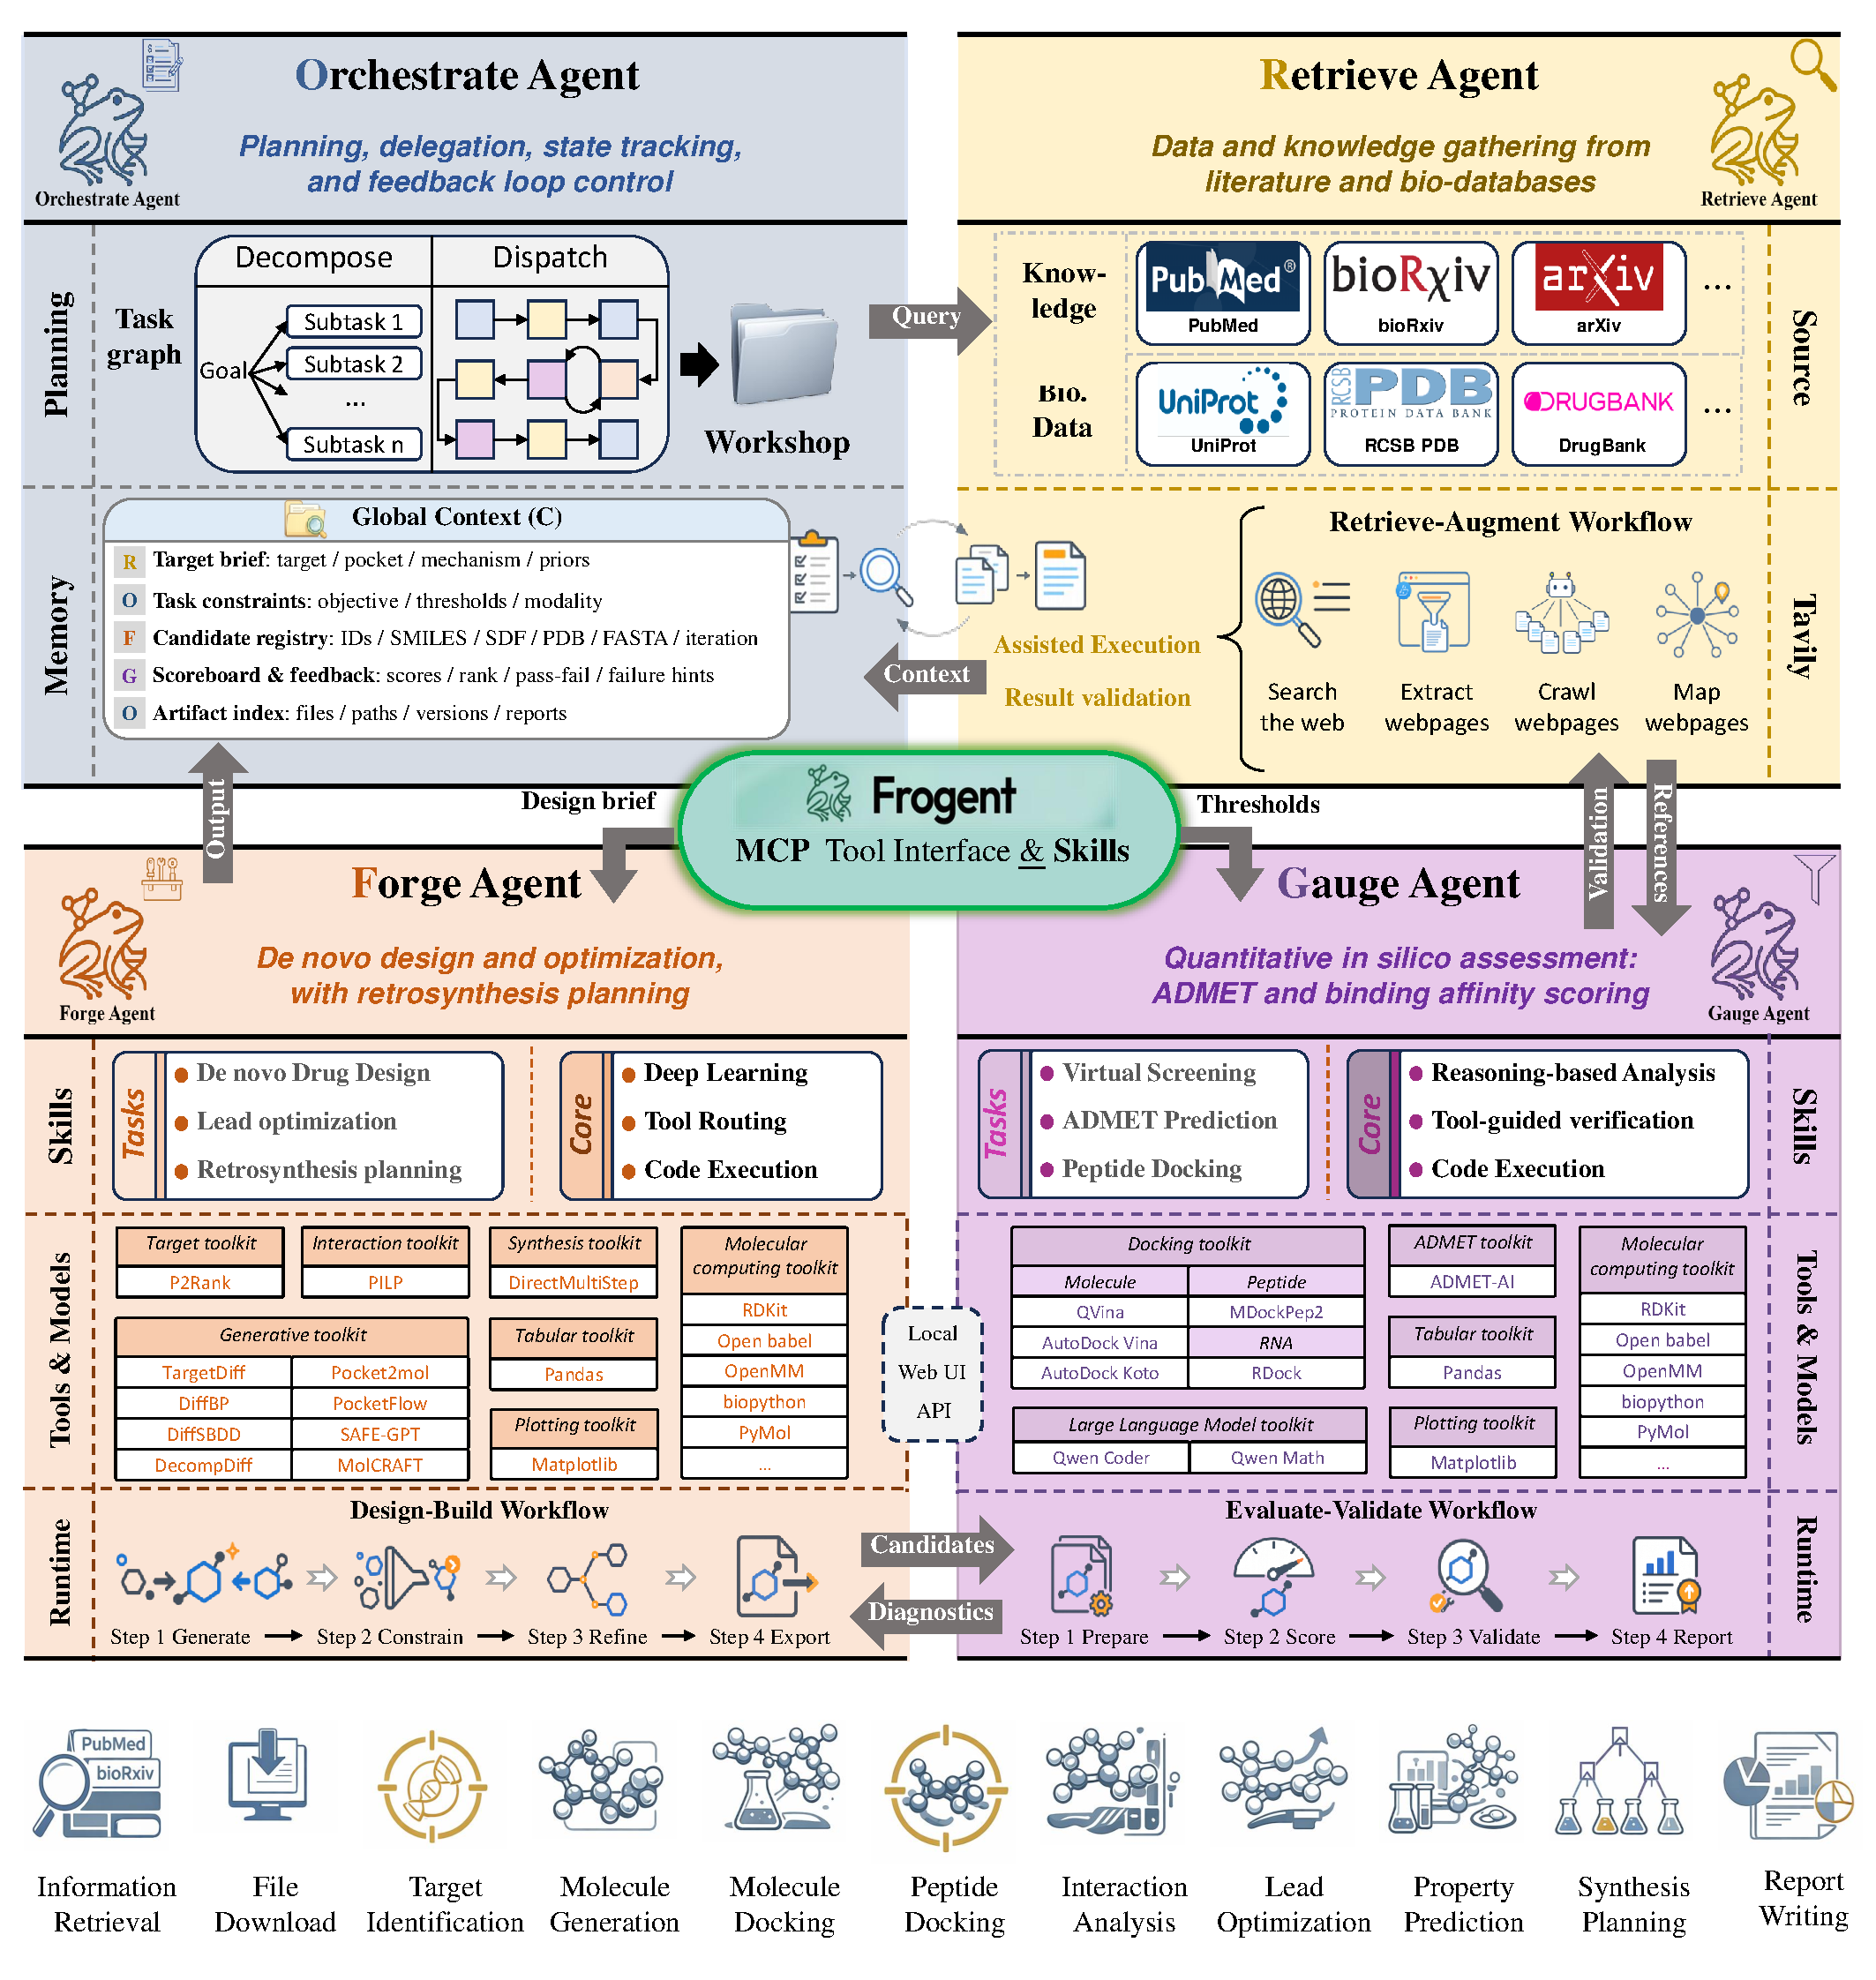
\includegraphics[width=1.0\textwidth]{figures/frogent-arch.pdf}
\caption{\textbf{Architectural Overview of the \name Multi-Agent System.}
The system comprises four distinct agents coordinated by a central \oa \ that handles planning, delegation, and feedback loop control. The \ra \ gathers evidence from literature and verified biological-data paths. The \fa \ routes molecular generation, optimization, and retrosynthesis planning tasks. The \ga \ computes task-specific property, docking, geometry, and interaction signals. The bottom panel summarizes the implemented workflow categories; provider availability and validation scope are reported separately.}
\label{fig:Architecture}
\end{figure}

The \ra functions as the framework's epistemic module, responsible for foundational capabilities such as Information Retrieval and File Download. In response to queries from the \oa \ or other peer agents, it performs data and knowledge gathering by leveraging its access to both static knowledge bases and a dynamic Retrieve-Augment Workflow. This workflow enhances its capabilities with real-time web searching, webpage extraction, and content mapping to incorporate emergent information, which is then used for both task execution and result validation. A key application of this agent is in Target Identification, where it performs iterative searches to identify and prioritize disease-relevant targets based on scientific literature and biological databases.

The \fa \ acts as the framework's creative core, executing its primary tasks, Molecule Generation, Lead Optimization, and Synthesis Planning, through a synergy of Deep Learning, Tool Routing, and Code Execution. To achieve this, its action space is equipped with an extensive toolkit, including protein pocket discovery tools, protein-ligand interaction analyzers, a suite of generative models, retrosynthesis planners, and a rich library of molecular computing and visualization tools.

Complementing the generative capabilities is the \ga, which computes candidate-ranking signals for Molecule Docking, Peptide Docking, Property Prediction, and Interaction Analysis through code execution and tool-guided assessment. The \fa--\ga workflow supports design--evaluate--refine cycles in which generated candidates receive task-specific computational scores and those results can guide a subsequent allocation or design step. The matched-budget study evaluates one such feedback-allocation round; it does not treat docking or structure scores as experimental validation.

Coordinated by the \oa, the specialists execute the multi-stage computational workflow illustrated in Figure~\ref{fig:overview}. The \oa \ decomposes a high-level goal, delegates each stage, maintains shared context, and synthesizes returned evidence and tool outputs. Specialized agents can invoke their configured tools or request a typed subtask from a peer agent. Human oversight remains available at campaign-defining decisions and for interpreting computational candidates.

\begin{figure}[htbp]
\centering 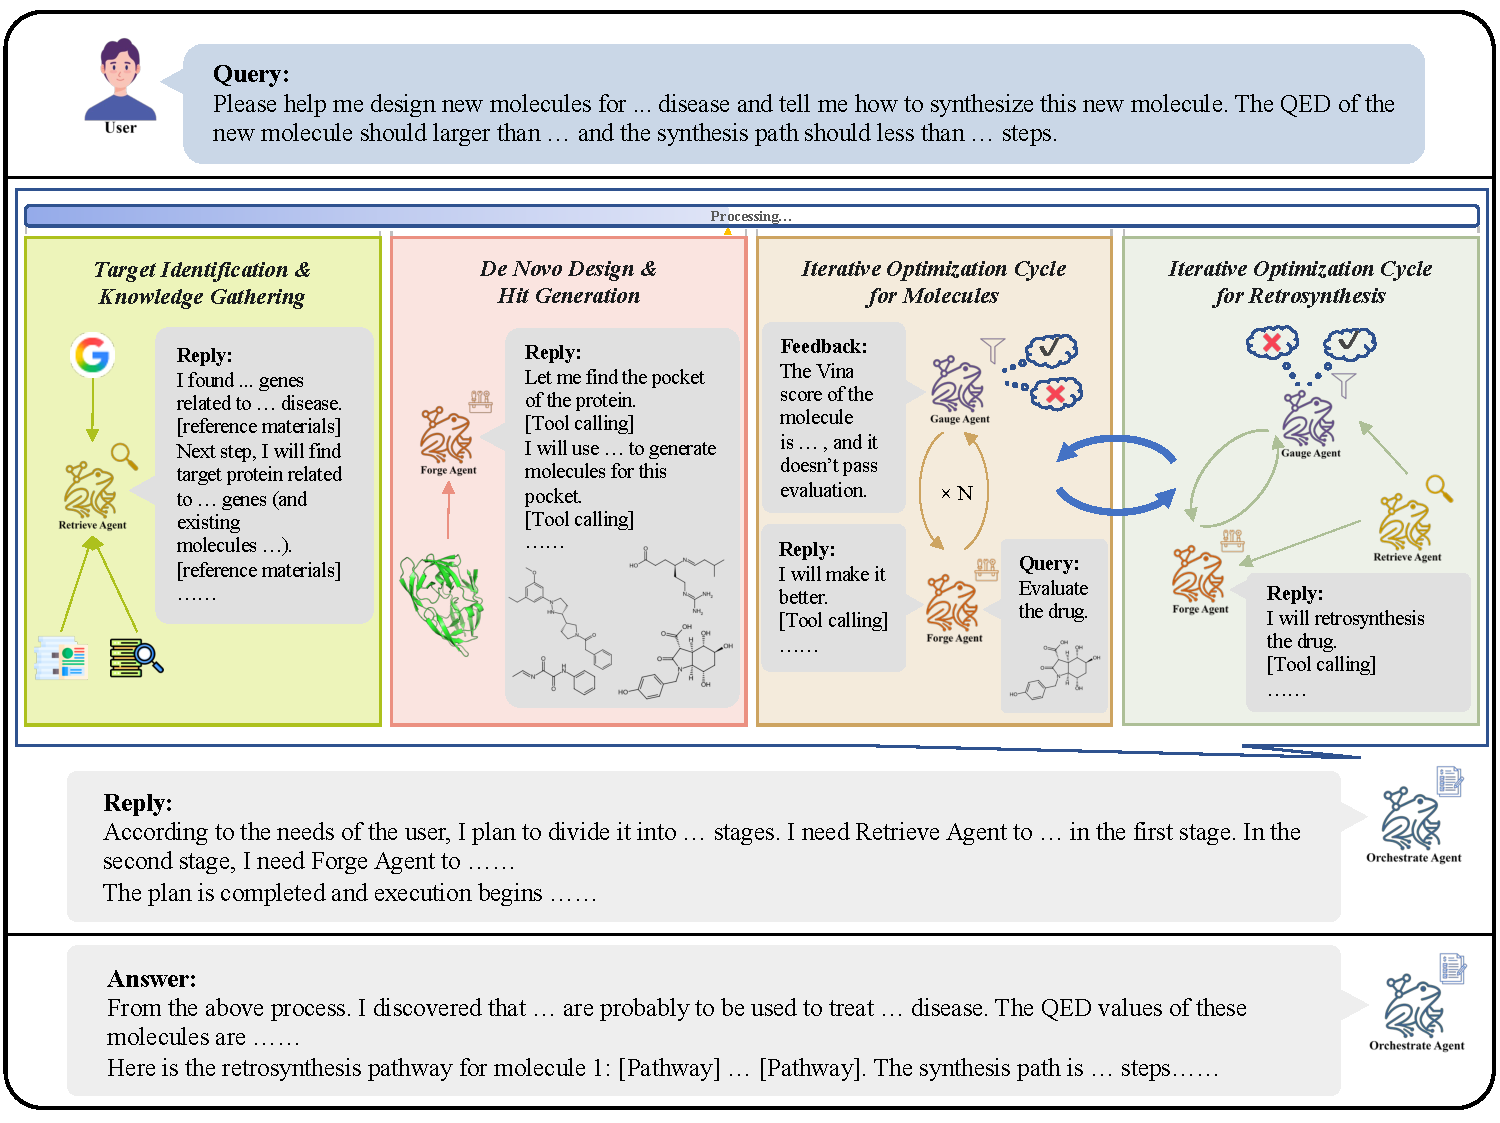
\includegraphics[width=1\textwidth]{figures/fig1-overview.pdf}
\caption{\textbf{Conceptual workflow of \nam.}
The \oa \ coordinates a multi-stage drug discovery campaign initiated by a single user query. The workflow progresses from initial knowledge gathering and hit generation to the core iterative optimization cycles, where collaboration between the \fa \ and \ga \ refines both molecular properties and synthetic feasibility before the \oa \ synthesizes a final solution.}
\label{fig:overview}
\end{figure}

\subsection*{Evaluation}

The submitted evaluation comprised eight 20-case tasks and six agent configurations. The revision received the case inputs and reference answers, but the original sample-level outputs, failures, seeds, scorer code, judge records, and task-version metadata were unavailable. We therefore withdrew the unreproduced aggregate superiority claims and treated all newly executed results as post-hoc exposed-case or independent tool-validation panels. Table~\ref{tab:revised-evaluation} reports the evidence that can be reproduced from the supplied cases and frozen revision protocols.

\begin{table*}[htbp]
\centering
\small
\caption{\textbf{Reproducible revision evidence for the eight submitted task categories.} Original headline scores and cross-agent rankings are excluded because their execution and scoring records were unavailable. Each result below states its own evaluation unit and scope.}
\label{tab:revised-evaluation}
\begin{tabular}{p{0.20\textwidth}p{0.48\textwidth}p{0.24\textwidth}}
\toprule
Task category & Reproduced or independent revision evidence & Interpretation boundary \\
\midrule
Foundational biomedical knowledge & Luna/max completed 20/20 exposed no-tool cases; exact accuracy was 9/20 (0.450; Wilson 95\% CI, 0.258--0.658). & Official HLE identity and the submitted score are not reproduced. \\
Known-drug and known-target retrieval & Removing Retrieve reduced score by 7.000/10 over five matched retrieval cases (95\% CI, 5.200--8.500); live evidence tests retained provenance and revocation behavior. & Applies to tested retrieval cases and verified sources. \\
Molecular properties & RDKit QED matched 20/20 supplied values at three decimals. Caco-2 $\rho=0.501$; BBBP, CYP2D6-sub, and SR-p53 balanced accuracy was 0.550, 0.786, and 0.472. & Endpoints are reported separately; the submitted aggregate is not reproduced. \\
Virtual screening & The FROGENT wrapper matched direct Vina scores for ten ABL1 ligands; score-versus-DAVIS rank correlation was $\rho=0.115$ ($p=0.751$). & Supports faithful tool execution, with weak affinity discrimination in this panel. \\
Interaction profiling & Direct and adapter PLIP XML agreed in 12/12 cases; typed end-to-end exact rate was 0.667. & Metal and water-bridge fields remain unsupported schema classes. \\
Molecular generation & CBGBench primary, extension, and pooled matrices completed 45/45, 45/45, and 90/90 jobs; TargetDiff ranked highest in valid rate and QED under this protocol. & Results are model-, pocket-, seed-, and metric-specific computational comparisons. \\
Retrosynthesis & DirectMultiStep returned nonempty, target-rooted, parse-valid routes for 40/40 calls; flash/explorer mean top-5 exact-reference reaction recall was 0.572/0.738. & Alternative-route equivalence awaits blinded adjudication; the submitted headline is not reproduced. \\
\bottomrule
\end{tabular}
\end{table*}

The revised evidence identifies two distinct signals. Retrieval access and evidence handling contributed strongly on the matched retrieval cases, whereas computational tools showed provider-specific strengths and failure modes. QED was deterministic, ADMET performance varied by endpoint, the docking wrapper reproduced direct Vina output while the score weakly tracked experimental affinity, and the typed PLIP path exposed defined schema gaps. These findings support tool-use reliability and explicit error accounting within the tested settings.

For structure-based generation, the three executable manuscript-scope models---TargetDiff, DiffSBDD, and Pocket2Mol---were compared across five pockets and six seeds. TargetDiff retained the highest valid-rate and QED ranking, while Pocket2Mol produced the easiest SA scores under the conventional lower-is-better direction. A separate matched-budget study showed that one Forge--Gauge feedback allocation round improved valid rate over uniform single-pass allocation, while known fixed-best TargetDiff retained a validity advantage. The retrosynthesis panel establishes executable, parse-valid route generation and conservative exact-reference coverage; chemical equivalence of alternative routes requires separate adjudication.

Three recent public systems were additionally installed at frozen commits and evaluated as current-model workflow adaptations on the subset of exposed tasks with aligned inputs, outputs, and scorers (Figure~\ref{fig:external-adaptations}). CLADD, Prompt-to-Pill, and Robin all used GPT-5.6 Sol as the current base model, with access to each system's frozen public files, available native components, and public web resources; FROGENT used its selected base-model configuration. Resource-audited recovery completed all six aligned cells. CLADD scored 0.824 on molecular-property prediction. Its public executable interface supports molecule-centred property prediction and drug--target inference from a supplied molecule--target pair; it does not expose the pocket-based screening, de novo generation, target-to-known-drug retrieval, or disease-to-target output contracts used in the other four columns. Prompt-to-Pill scored 0.854, 0.895, and 0.838 on property prediction, virtual screening, and molecular design. Its public workflow begins from a supplied UniProt target and provides molecular generation, scoring, and optimization tools; it contains no target-to-DrugBank retrieval or disease-to-target discovery path. Robin scored 0.665 and 0.283 on known-drug and known-target retrieval. Its public computational workflow begins from a disease name and uses literature-grounded hypothesis generation to propose assays and therapeutic candidates; it contains no molecule-specific property predictor, pocket-based screening engine, or de novo molecular generator. The comparison displays all 12 direct LLMs individually. FROGENT obtained 0.833, 0.842, 0.931, 0.930, and 0.800 across the five displayed tasks. The retrieval cells bind canonical Open Targets associations and reviewed UniProtKB DrugBank cross-references directly after typed validation, while the selected base-model configuration handles planning, ambiguity and scientific interpretation. FROGENT therefore led the aligned molecular-design and retrieval cells; Prompt-to-Pill retained the higher property and virtual-screening scores.

\begin{figure*}[htbp]
\centering
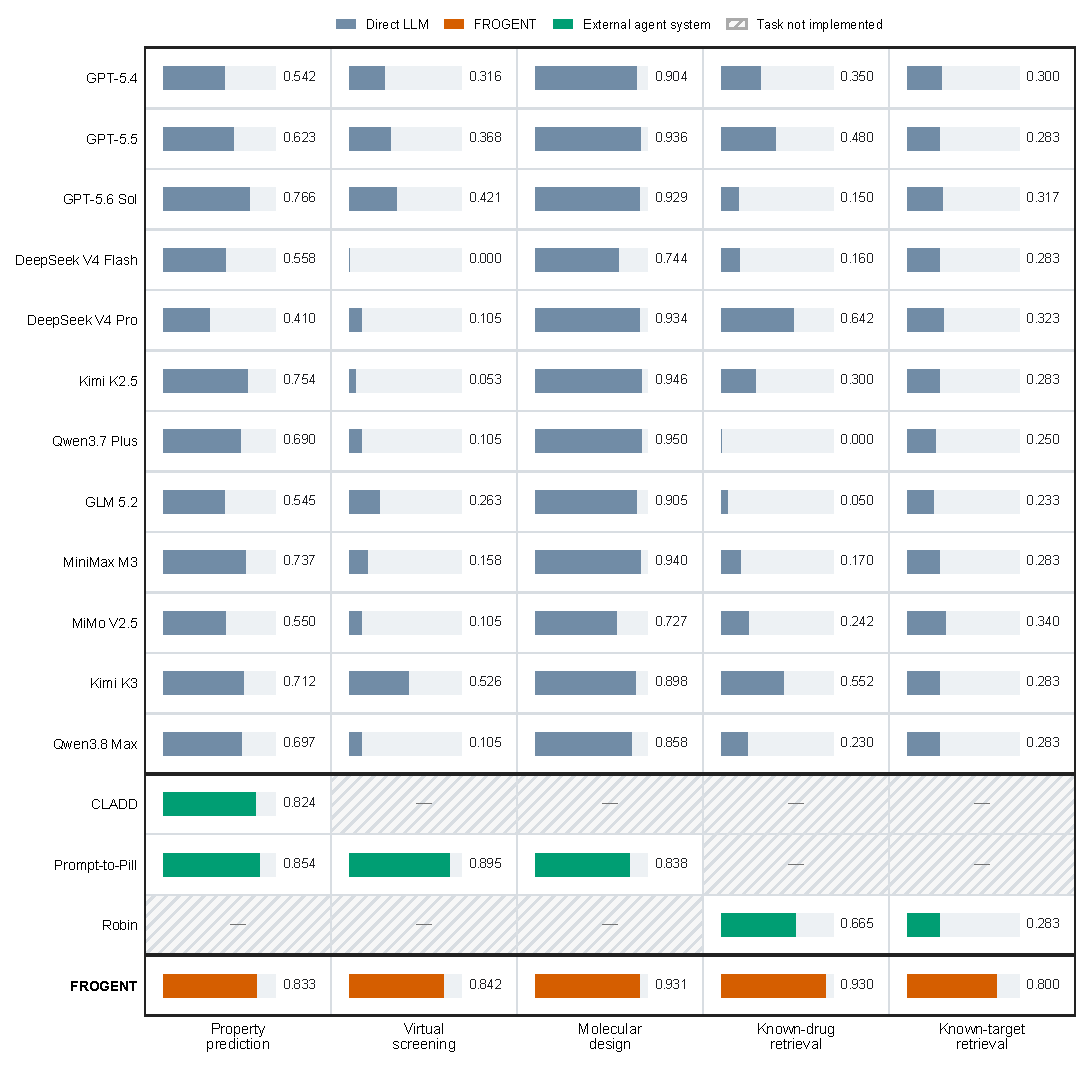
\includegraphics[width=0.98\textwidth]{figures/external-current-model-adaptations.pdf}
\caption{\textbf{Task-aligned comparison across direct LLMs and agent systems.} Bar length and the printed value report the task-specific score. The 12 direct LLMs are displayed individually, followed by CLADD, Prompt-to-Pill, Robin, and FROGENT in the bottom row. Each measured cell contains 20 exposed cases, except virtual screening with 19 valid cases. Hatched cells mark tasks absent from the corresponding public workflow.}
\label{fig:external-adaptations}
\end{figure*}

\subsection*{Case Studies}

We present three representative computational case studies spanning known-candidate evidence recovery, small-molecule generation and synthesis planning, peptide prioritization, and lead-editing workflows. Each case traces the participating agents, provider outputs, and the evidence boundary applied to the resulting candidates.

\subsubsection*{End-to-End Drug Design for Cardiomegaly-congestive Heart Failure}
\label{case: 1}
Target discovery forms the foundation of modern pharmaceutical research. However, it remains a leading cause of failure in late-stage clinical trials due to inadequate validation or selection of non-actionable targets \cite{waring2015analysis, hughes2011principles}. A pipeline that couples target discovery with downstream design tasks can address this challenge by aligning molecular generation efforts with validated mechanisms from the outset \cite{mak2024artificial}.

To evaluate this collaborative capability, we initiated a comprehensive discovery cycle for cardiomegaly and congestive heart failure, as depicted in Figure \ref{fig:pipeline}. The process began when the \oa \ received the user's broad query. It first tasked the \ra \ to perform a comprehensive literature and database search, which identified PPAR$\alpha$, PPAR$\gamma$, and Mineralocorticoid Receptor as relevant nuclear receptor targets. Subsequently, guided by the user's prioritization of PPAR$\gamma$ as the target receptor  for the entire design process, the \oa \ directed the \ra \ to secure a high-resolution crystal structure (PDB ID: 9F7W).

With the target structure obtained, the \oa \ formulated a design plan and tasked the \fa \ to generate candidate molecules. The \ra \ supplied literature and known-candidate context, and the \fa \ generated pocket-conditioned structures. The candidate library was passed to the \ga \ for RDKit descriptors, ADMET predictions, docking scores, and geometry checks. These computational signals supplied a ranked shortlist and feedback for fragment-level modifications; they were not interpreted as measured affinity or efficacy.

The workflow retrieved Luteolin as a previously reported candidate and linked it to DrugBank DB15584, PubChem CID 5280445, ChEMBL CHEMBL151, ChEBI CHEBI:15864, and preclinical PPAR$\gamma$ evidence in cardiomyocyte and mouse models \cite{wang2023high}. A literature-only arm recovered the cited mechanism without structured drug--target or drug--indication relations, establishing evidence recovery with an exposed candidate rather than blinded candidate discovery. In parallel, the workflow generated Compound (a), prioritized it using the reported computational property and docking signals, and produced a candidate retrosynthesis plan. Experimental efficacy, binding affinity, and synthetic validation were not measured.

\begin{figure}[t]
\centering 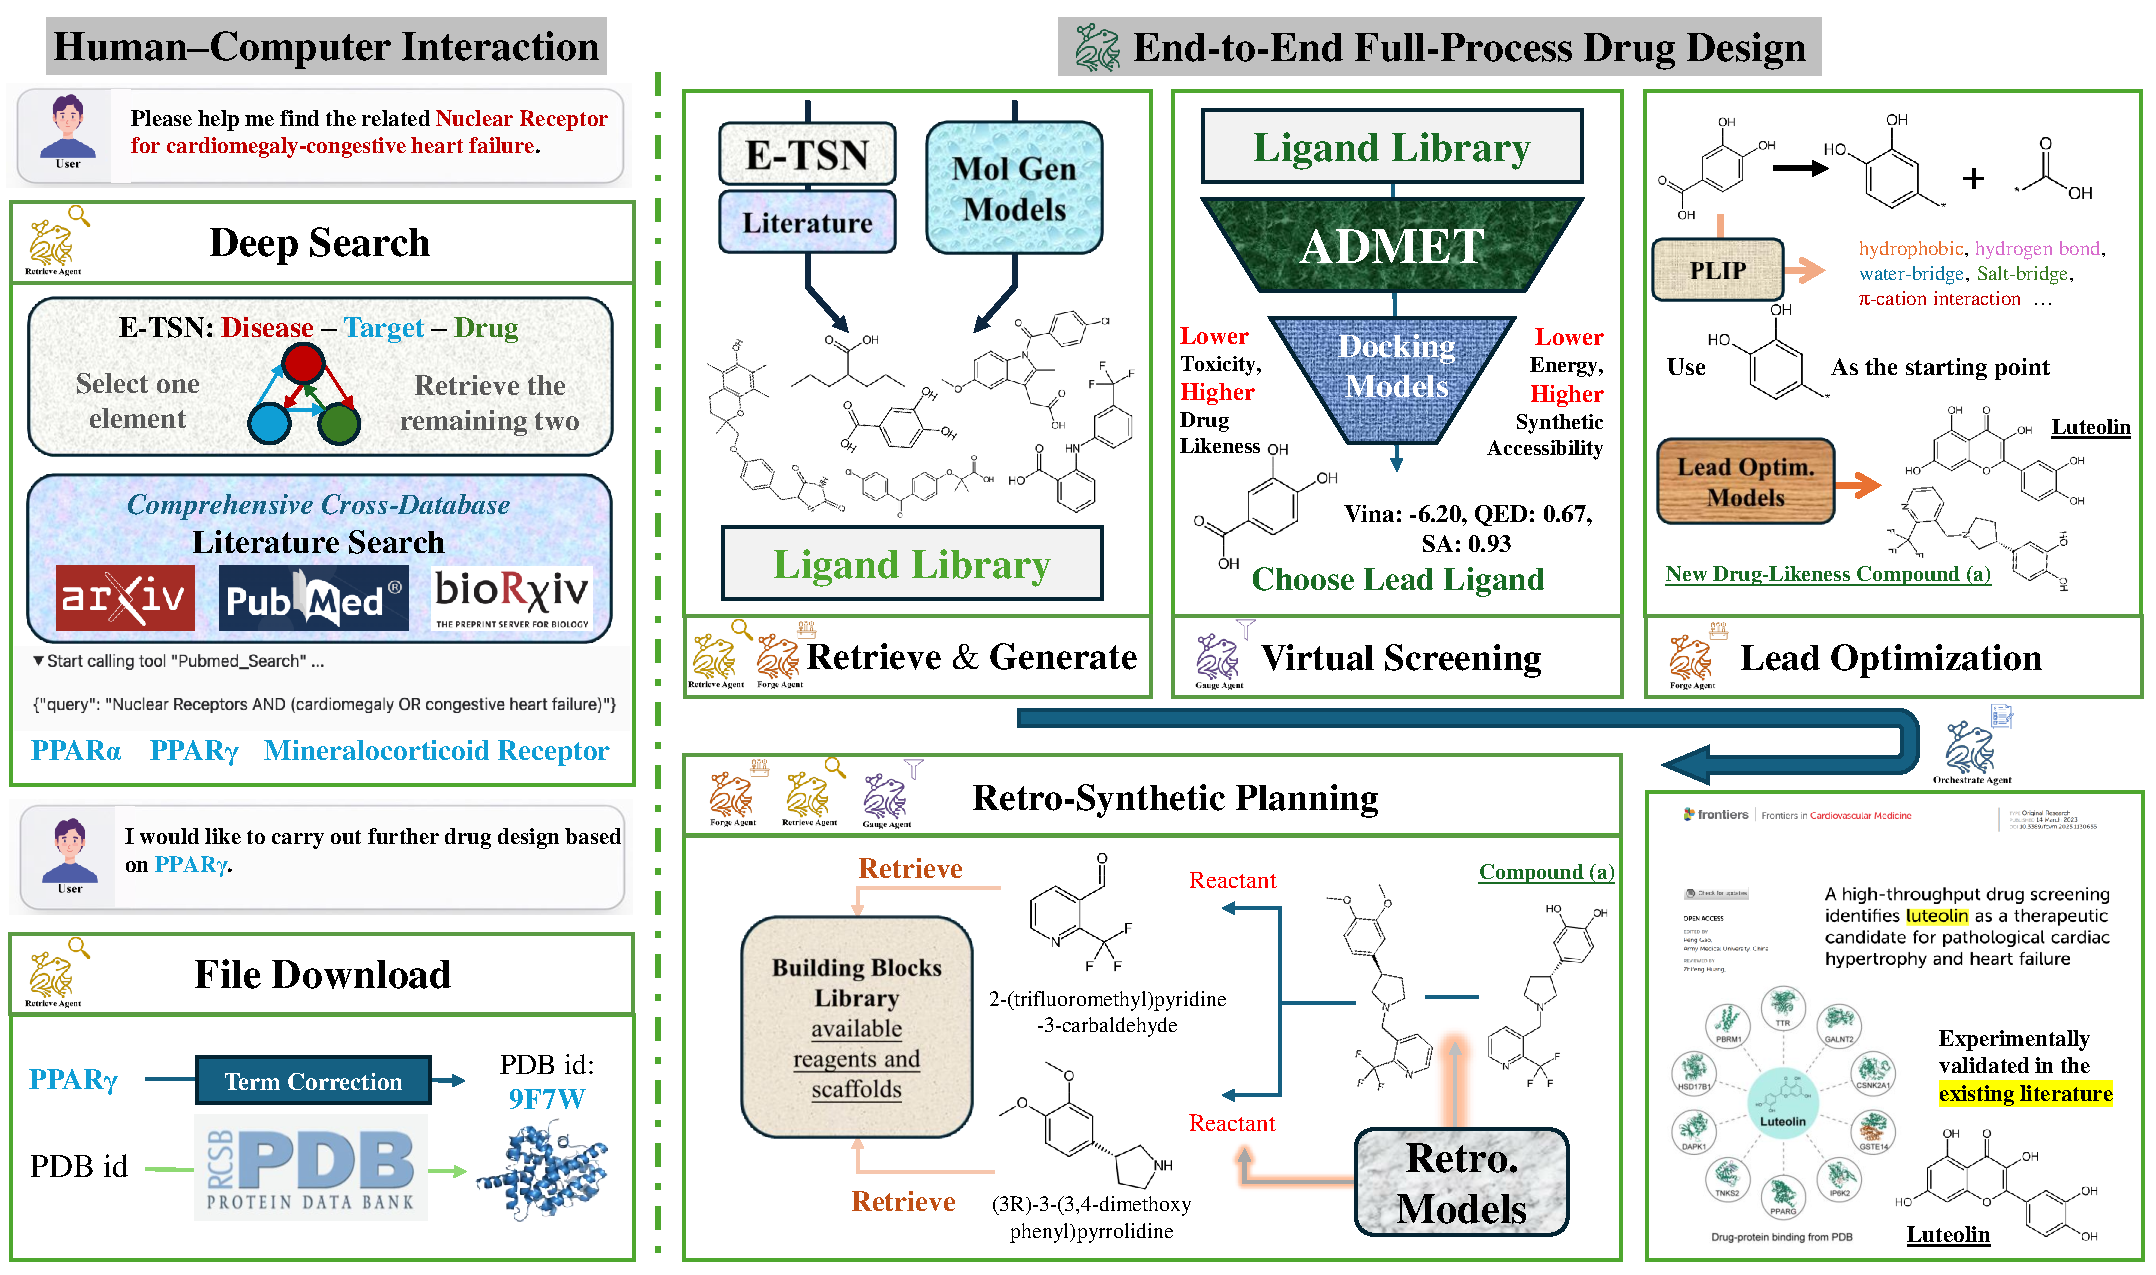
\includegraphics[width=1.0\textwidth]{figures/fig3-pipeline.pdf}
\caption{\textbf{End-to-End Drug Design for Cardiomegaly-congestive Heart Failure.}
Following a user query, the \oa \ tasks the \ra \ to identify PPAR$\gamma$ as a relevant target, which provides context for the \fa \ to generate candidate molecules. The workflow retrieves Luteolin as a known candidate with traceable preclinical evidence, applies computational prioritization to generated molecules, and proposes a retrosynthesis plan for Compound (a).}
\label{fig:pipeline}
\end{figure}

\subsubsection*{Lead Optimization for Glucagon-Like Peptide 1 Receptor}
\label{case: 2}
Peptide therapeutics represent a rapidly growing class of drugs, but issues of binding affinity, stability, and selectivity often challenge their development \cite{kumar2023recent}. The optimization of a native peptide sequence to enhance its interaction with a target receptor is a critical and complex task in modern drug discovery \cite{lee2019comprehensive}.

To evaluate the peptide branch, we used GLP1R structural context (PDB ID: 4ZGM) and the Glucagon sequence to generate targeted in silico variants. Candidate ordering used computational structure and docking signals as prioritization features. These scores were not interpreted as binding affinity or potency.

Independent structural panels bounded this workflow. ADCP completed 9/9 reference-redocking tasks, with mean top-1/top-5/top-10 backbone RMSD of 11.262/5.840/4.690~\AA\ and corresponding native-contact recovery of 0.271/0.564/0.593. Direct licensed MDockPeP2 completed 3/3 reference complexes; top-ranked receptor-frame peptide CA RMSD was 2.479/13.546/17.123~\AA\ for 3GBQ/1CKB/1ABO, whereas best-of-100 RMSD was 2.225/2.336/4.564~\AA. ESMFold and AlphaFold3 disagreed substantially on the tested peptide poses (mean cross-provider pose difference, 31.513~\AA). These results demonstrate executable multi-provider structural prioritization and expose weak cross-complex pose ranking; experimental activity, affinity and broad docking superiority remain outside the claim.

\begin{figure}[t]
\centering 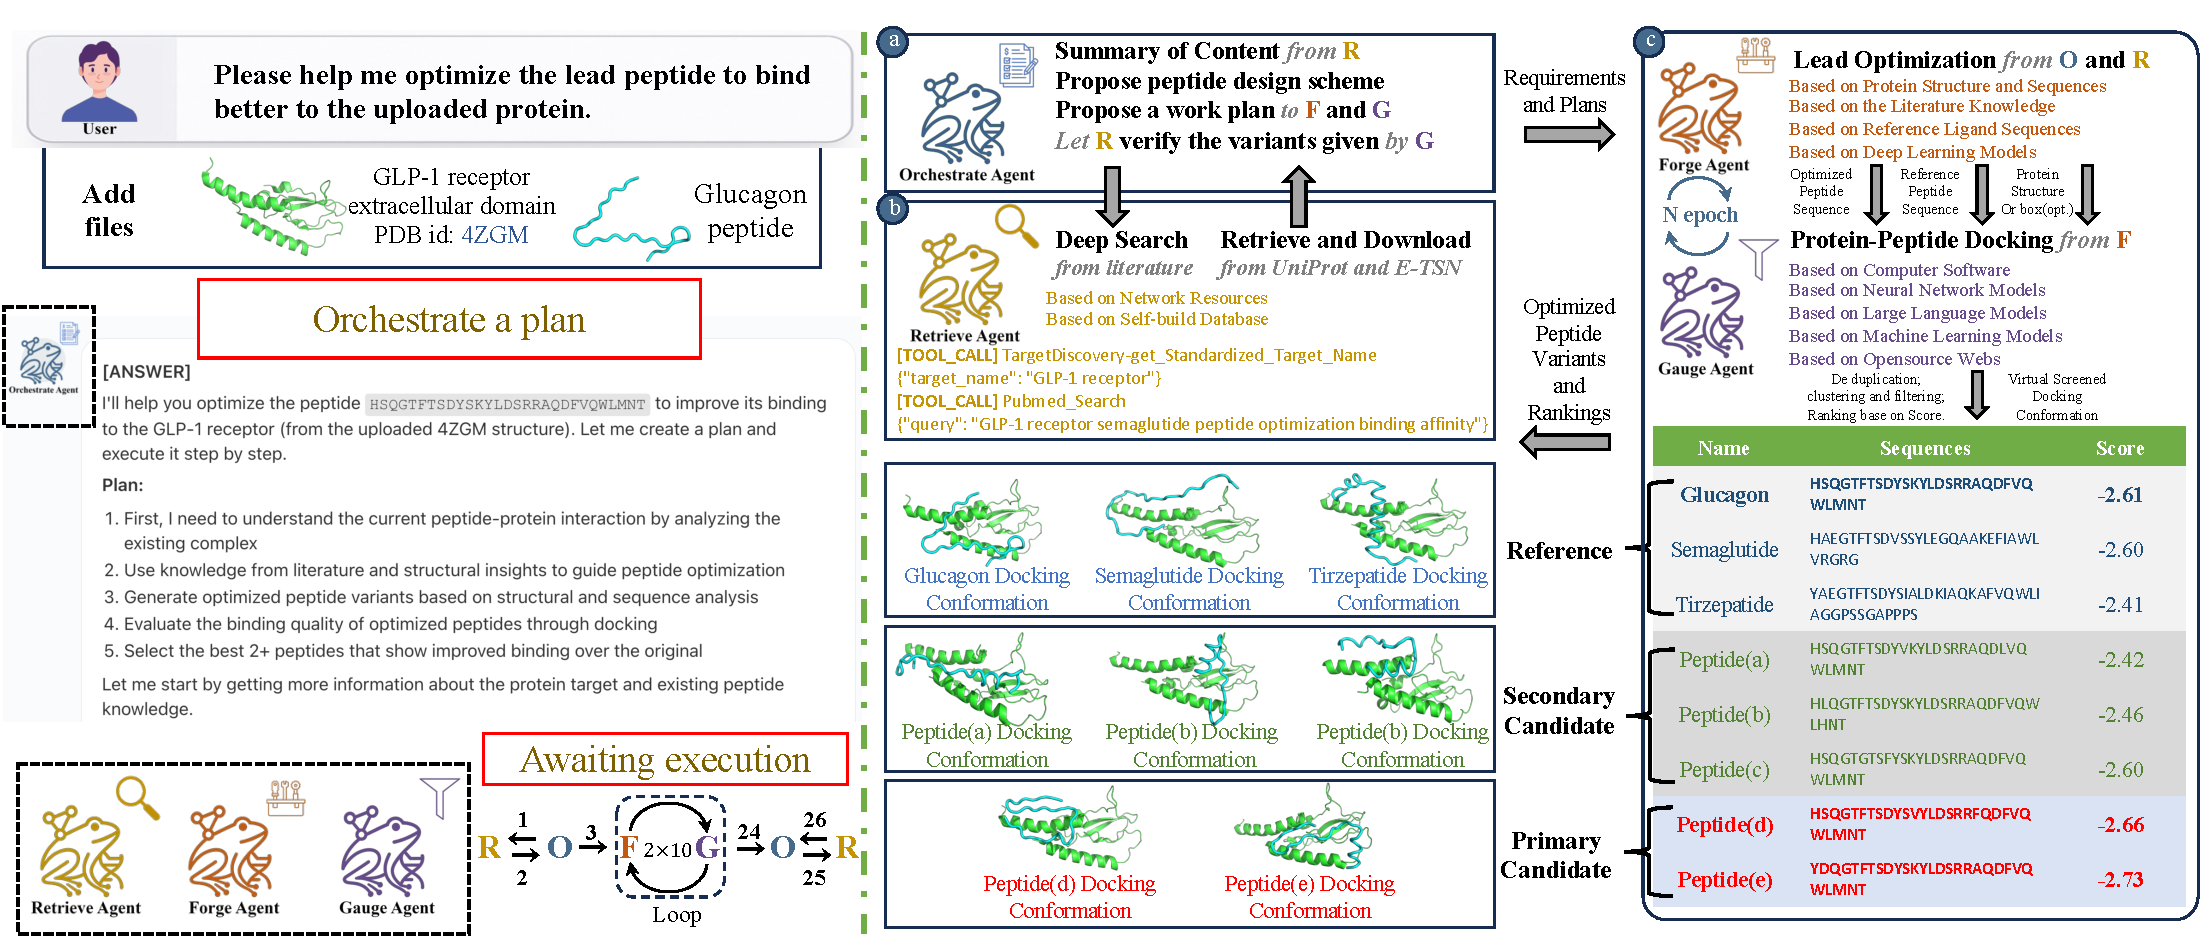
\includegraphics[width=1.0\textwidth]{figures/fig4-OptPep.pdf}
\caption{\textbf{Computational peptide-design workflow for Glucagon-Like Peptide 1 Receptor.}
The \oa \ acquires GLP1R structural context and the Glucagon sequence, the \fa \ generates peptide variants, and the \ga \ returns computational structure and docking signals for prioritization. Independent ADCP, direct licensed MDockPeP2, ESMFold and AlphaFold3 analyses define the structural reliability boundary; the displayed scores do not measure binding affinity, potency, or superiority over approved agonists.}
\label{fig:LeadOptimizationsPep}
\end{figure}

\subsubsection*{Lead Optimization for Carbonic Anhydrase Inhibitors}
\label{case: 3}
Lead optimization is a resource-intensive phase that transforms initial hit compounds into drug candidates with balanced potency, selectivity, and drug-like properties \cite{wager2010defining, gleeson2011probing}. This stage often demands iterative structure refinement guided by a complex interplay of biological and chemical considerations.

We assessed \nam's collaborative capability in this context by providing the \oa \ with a known N-substituted sulfonamide inhibitor targeting human Carbonic Anhydrase II (CAH II, PDB ID: 3K34), as shown in Figure \ref{fig:LeadOptimizationsMol}. The \oa \ first tasked the \fa \ to perform a detailed structural analysis, identifying key binding features and solvent-exposed regions suitable for modification. Based on this analysis, the \oa \ initiated the core optimization loop. It directed the \fa \ to use its fragment-based generative models to propose a focused library of new analogues. This library was then passed to the \ga \ for comprehensive evaluation, including virtual screening, ADMET assessment, and redocking.

The \ga \ returned a computational ranking in which Compound (b) had the most favorable combination of the reported docking and ADMET signals. The \oa \ then directed the \fa \ to assess synthetic accessibility. DirectMultiStep produced an initial route whose proposed precursors were absent from the configured purchasable-building-block check, triggering a repair step.

The \oa \ initiated a synthesis-repair subtask, asking the \ra \ for documented transformations involving related motifs and PaRoutes context \cite{genheden2022paroutes}. The \fa \ then proposed two alternative routes using building blocks present in the configured catalogue. One route aligned at the transformation level with a published synthesis \cite{babalola2024design}. This case supports retrieval-assisted route repair; route feasibility for Compound (b) remains a computational proposal pending experimental execution.

\begin{figure}[t]
\centering 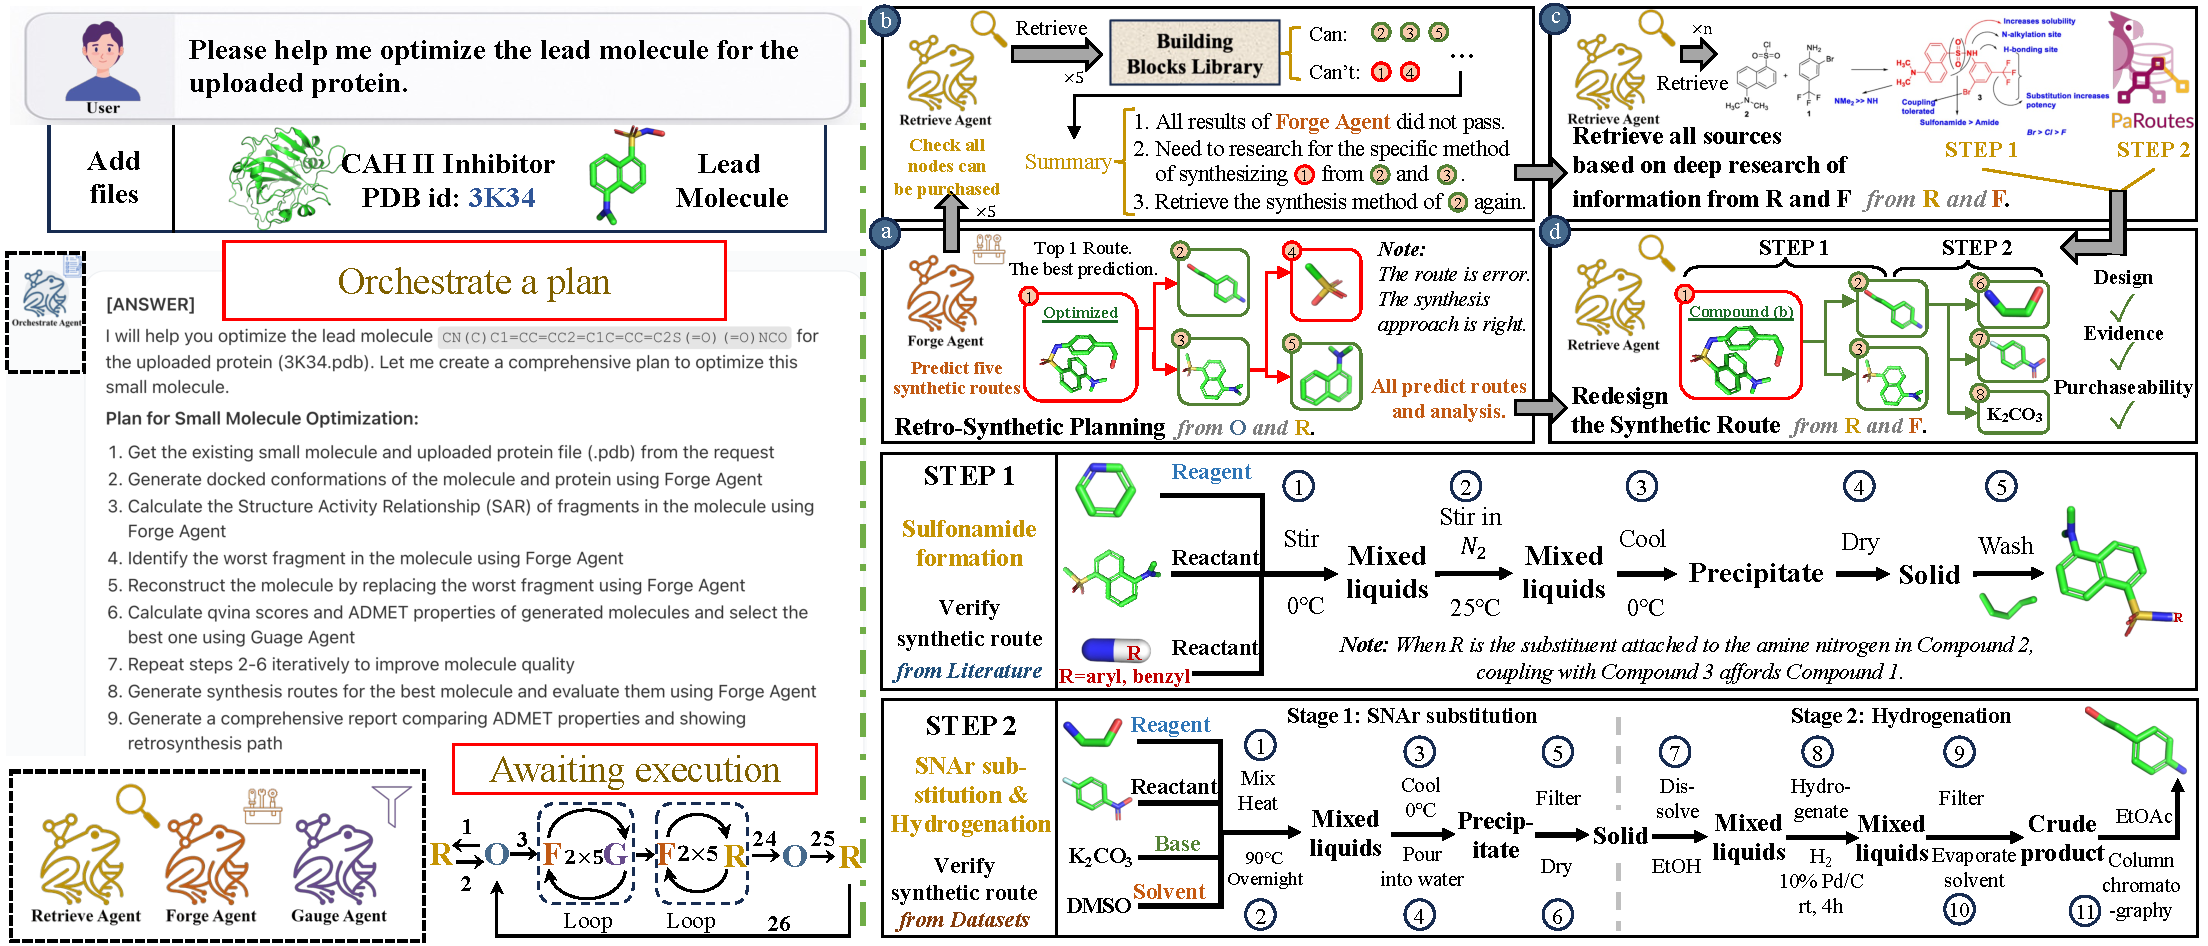
\includegraphics[width=1.0\textwidth]{figures/fig5-OptMol.pdf}
\caption{\textbf{Lead Optimization for Carbonic Anhydrase Inhibitors.}
Starting with a known lead molecule, the agents analyze and rank a generated analogue library using computational docking and property signals. Compound (b) is the highest-ranked candidate under the reported criteria. A failed purchasable-building-block check triggers retrieval-assisted route repair, producing two candidate routes, one of which aligns at the transformation level with a published synthesis. Experimental affinity, ADMET, and synthetic execution are not measured.}
\label{fig:LeadOptimizationsMol}
\end{figure}

\section*{Discussion}

\subsection*{LLM-driven Autonomous Agents}
The emergence of LLM-driven autonomous agents represents a significant paradigm shift, extending the capabilities of Large Language Models(LLMs) beyond static text generation to dynamic, goal-oriented problem-solving. At their core, these agents are architected to perform complex reasoning, formulate multi-step plans, and interact with external environments through tool use. Pioneering frameworks such as ReAct \cite{yao2023react} established a powerful methodology by prompting LLMs to interleave reasoning "thoughts" with concrete "actions", creating a synergistic and interpretable loop of planning and execution. Works like Toolformer \cite{schick2023toolformer} further solidified this fundamental ability to interact with the external world. Gorilla \cite{patil2024gorilla} demonstrated that LLMs can be effectively trained to master the use of external APIs, grounding their abstract reasoning in executable, real-world functions. Building upon these single-agent foundations, the field has progressed toward multi-agent systems (MAS), where collaboration is key to solving even more complex challenges. Frameworks like AgentVerse \cite{chen2023agentverse} and MetaGPT \cite{hong2023metagpt} showcase how intricate tasks can be decomposed and assigned to a cohort of specialized agents that collaborate, much like a human team, to achieve a common goal. However, while these general-purpose agentic frameworks provide a powerful blueprint for autonomous systems, they inherently lack the deep domain knowledge and fine-grained, validated toolsets essential for navigating the complexities of specialized scientific domains such as drug discovery. Their effectiveness is contingent on the availability of generic tools, which fall short of the requirements for high-stakes, precision-oriented scientific research.


\subsection*{Agents in Drug Discovery}
The transformative potential of AI has spurred the development of specialized agents tailored for various facets of drug discovery, each addressing specific and complex challenges within the pipeline. For instance, ChemCrow \cite{bran2023chemcrow} demonstrated significant capabilities by augmenting an LLM with a suite of chemistry-focused tools, enabling it to plan and execute tasks in organic synthesis and drug design effectively. In a parallel effort, DrugAgent \cite{liu2024drugagent} focuses on a different yet equally critical bottleneck: automating the machine learning (ML) programming required for drug discovery tasks, acting as an agent that can write, debug, and execute experimental code. In a more interactive paradigm, ChatMol Copilot \cite{sun2024chatmol} serves as a user-centric assistant, translating natural language instructions into complex molecular modeling and computational commands, thereby lowering the barrier for researchers to access sophisticated simulation tools.

Recent systems cover complementary portions of agentic drug discovery. CLADD combines collaborative molecular RAG, biomedical knowledge graphs, and specialized routing for target and property-oriented inference \cite{lee2025rag}. Prompt-to-Pill connects molecular generation, docking, ADMET, optimization, and clinical-simulation components in a DPP-4 proof of concept \cite{vichentijevikj2026prompt}. Robin links literature-grounded hypothesis generation to human-executed experiments, experimental-data analysis, and iterative hypothesis refinement \cite{ghareeb2026robin}. These systems overlap substantially with different parts of the FROGENT workflow. We compare released capabilities qualitatively and report current-model numerical adaptations only for the six task cells with matched exposed inputs and frozen scorers. Unavailable legacy components, wet-lab stages, and non-alignable cells remain unmeasured.

\subsection*{Limitations}
While \name demonstrates a significant advance in automating the drug discovery workflow, its efficacy is intrinsically linked to the capabilities of its foundational components. The system's reasoning and scientific knowledge are fundamentally bounded by the fidelity of its core LLM, which can still exhibit hallucinations or flawed logic when faced with complex scientific problems. While our multi-agent architecture is designed to mitigate such errors by grounding actions in tool-based observations, the system's ability to recover from a flawed plan is ultimately dependent on the LLM's reasoning fidelity. Looking forward, the continuous evolution of next-generation foundation models will be crucial for enhancing the system's robustness and scientific accuracy.

\begin{figure}[!h]
\centering 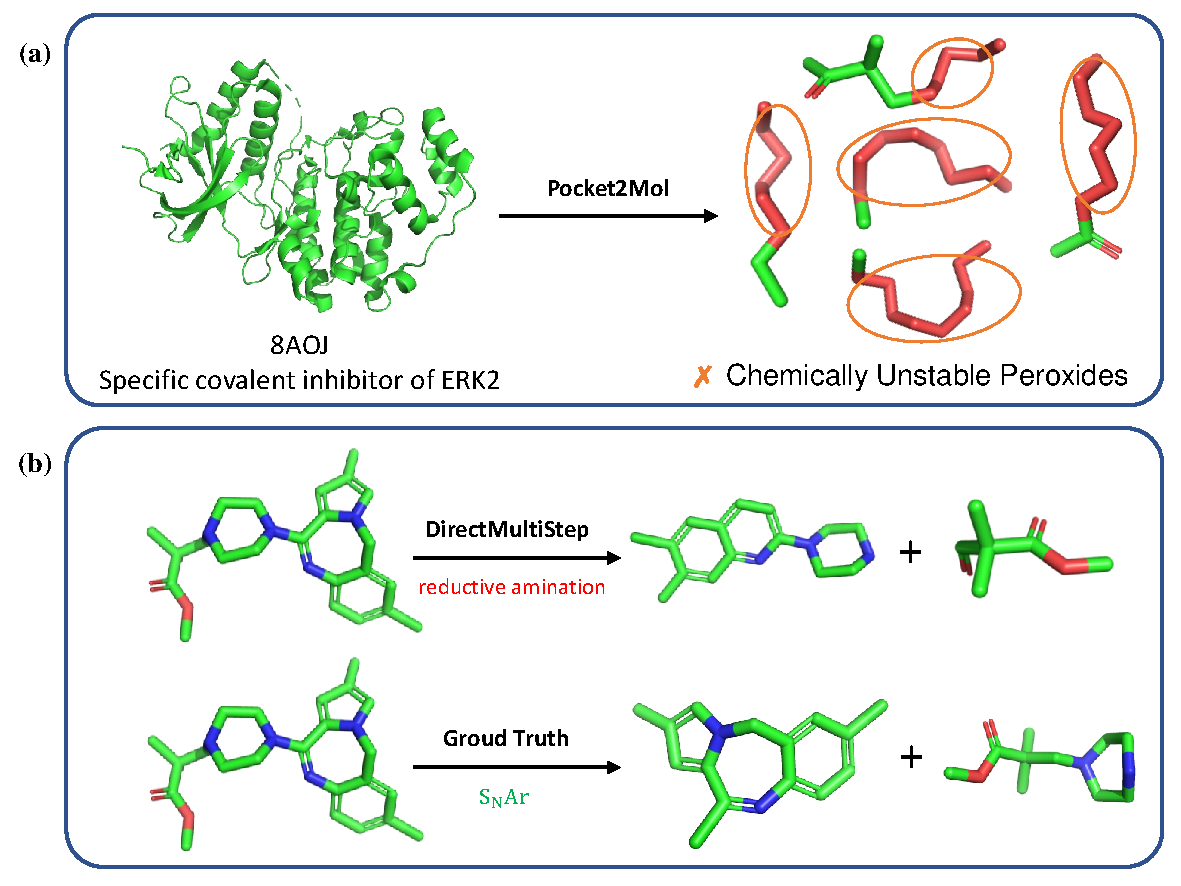
\includegraphics[width=0.8\textwidth]{figures/limitations.pdf}
\caption{\textbf{Illustrative Failure Cases of Integrated Scientific Tools.}
(a) A failure case of Pocket2Mol, where the model generated molecules containing chemically unstable peroxide groups when tasked with designing ligands for the ERK2 binding site (PDB: 8AOJ). (b) DirectMultiStep proposing a strategically flawed retrosynthesis via reductive amination, which relies on a more complex precursor than the target molecule, in contrast to the chemically sound Nucleophilic Aromatic Substitution (SNAr) ground truth. These examples highlight the dependency of \name on the fidelity of its specialized tools.}
\label{fig:Limitations}
\end{figure}

Similarly, its operational performance is directly contingent upon the accuracy and coverage of its specialized scientific tool suite.  For instance, in a de novo design task targeting the ERK2 protein (PDB: 8AOJ), we observed that the Pocket2Mol model generated a series of molecules containing chemically unstable peroxide groups, as illustrated in Figure \ref{fig:Limitations}(a). Similarly, while DirectMultiStep is a powerful retrosynthesis tool, it can propose chemically implausible reaction pathways. As shown in Figure \ref{fig:Limitations}(b), the tool proposed synthesizing a complex product via a reductive amination pathway that relied on an even more complex precursor. In contrast, the established chemical synthesis for this molecule proceeds via a Nucleophilic Aromatic Substitution (SNAr) reaction, coupling a piperazine ester with a reactive chloro-substituted heterocyclic core. DirectMultiStep's failure to identify this more conventional and efficient pathway highlights a gap in its ability to perform high-level strategic planning, even when the individual reaction step it proposes is chemically valid in principle. These specific failures underscore that \nam's performance is intrinsically linked to the strategic fidelity of its specialized tool suite. Future work will focus on integrating more sophisticated, consensus-based validation methods to enhance the reliability of the Gauge Agent.

Furthermore, a key limitation is that the entire \name workflow currently operates within a computational domain, creating an unavoidable gap between its predictions and real-world biological activity. The extensive use of multiple agents and advanced tools also incurs computational costs, which may limit accessibility. Looking forward, our vision is to bridge this silico-to-reality gap and address the cost by achieving a fully closed-loop discovery system. The most exciting future direction for \name is its integration with automated robotic platforms, which would enable a truly autonomous design-build-test-learn cycle.


\section*{Conclusion}
In this work, we presented \nam, a multi-agent platform that coordinates planning, evidence retrieval, molecular generation, computational evaluation, and retrosynthetic planning across small-molecule and peptide workflows. The experiments quantify strong retrieval dependence in the tested cases, a smaller and uncertain Gauge contribution, reproducible comparative behavior among three deployed generators, and a significant gain from one feedback-allocation round relative to uniform single-pass allocation. A known fixed-best generator retained the highest validity, and the remaining docking, peptide, and exposed benchmark results identify important provider and scoring limitations.

Together, these results support FROGENT as an integrated computational workflow for evidence-grounded task routing, scientific tool use, and feedback-based candidate allocation within the evaluated settings. Prospective experimental validation, broad affinity prediction, cross-system performance superiority, and reductions in development time or cost remain outside the present evidence.

%TC:ignore
\section*{Methods}

\subsection*{Multi-Agent Framework}
\label{sec:framework}

\subsubsection*{Orchestrate Agent}
The \oa \ serves as the central controller of the \name  framework, governing the state and execution flow of the entire drug discovery campaign. Leveraging the advanced reasoning capabilities of its underlying LLM, it employs a ReAct-style \cite{yao2023react} methodology for multi-step planning and task decomposition. It interprets high-level user goals expressed in natural language, breaks them down into executable subtasks dynamically, and assigns them to specialized agents. The \oa \ initiates the discovery process by first tasking the Retrieve Agent to gather foundational knowledge, from existing literature to known targets and compounds. Armed with this essential context, it formulates a precise design plan and directs the \fa \ to begin the creative design process. Subsequently, it synthesizes the outputs from all agents, facilitating a dynamic, closed-loop  "design-evaluate-refine" cycle. Feedback from the \ga \ is integrated to strategically guide the \fa \ in subsequent rounds of molecular design. Crucially, it serves as the primary interface for human oversight, presenting key findings and soliciting user input at critical decision points, promoting collaborative synergy.

\subsubsection*{Retrieve Agent}
The \ra \ functions as \nam's knowledge acquisition backbone, specializing in the retrieval and synthesis of information from diverse sources. The agent queries biomedical literature from key archives, including PubMed \cite{white2020pubmed}, BioRxiv \cite{sever2019biorxiv}, and ArXiv, and uses verified structured paths for RCSB PDB \cite{goodsell2020rcsb}, UniProt \cite{uniprot2025uniprot}, and Open Targets. E-TSN \cite{feng2022tsn}, Building Blocks \cite{BuildingBlocks2025}, and real-time Tavily search \cite{Tavily2025} provide task-dependent context where configured. Direct DrugBank \cite{knox2024drugbank} access returned HTTP 403 in the revision environment, so DrugBank-specific execution and performance were not evaluated.

\subsubsection*{Forge Agent}
The \fa \ is \nam's generative and synthesis-planning component. It can characterize binding sites with P2Rank \cite{krivak2018p2rank}, apply SAFE \cite{noutahi2024gotta} for lead-editing tasks, and route structure-based generation to the three models evaluated in this study: TargetDiff \cite{guan20233d}, Pocket2Mol \cite{peng2022pocket2mol}, and DiffSBDD \cite{schneuing2024structure}. DiffBP, MolCRAFT, DecompDiff, and PocketFlow were present in the submitted capability inventory but lacked verified executable checkpoints in the audited production roots and are treated as deferred. Generated structures can be analyzed with RDKit \cite{RDKit2025} and the supported PLIP \cite{salentin2015plip} fields. DirectMultiStep \cite{shee2025directmultistep} supplies candidate retrosynthesis routes, with exact-reference coverage and alternative-route adjudication reported separately.

\subsubsection*{Gauge Agent}
The \ga \ ranks and filters candidates using computational descriptors, ADMET-ai \cite{swanson2024admet}, small-molecule docking through QVina/Vina \cite{handoko2012quickvina}, structural-interaction analysis, and peptide-structure tools. Docking scores are treated as ranking and geometry signals because the tested Vina panel showed weak experimental-affinity discrimination. ADCP and direct licensed MDockPeP2 \cite{xu2021predicting} provide reference-redocking evidence. The failed historical MDockPeP2 endpoint canary and inconsistent direct top-1 ranking are retained as operational and structural limits.

\subsection*{Prompt Engineering Strategy}
Each agent receives a role-defining system prompt specifying responsibilities, available actions, output conventions, and operational constraints. FROGENT uses pretrained base models without task-specific parameter updates; specialization is implemented through role instructions, typed output schemas, evidence admission, and runtime tool access \cite{brown2020language, wei2022chain}. The active role contracts contain no benchmark demonstrations or task-specific few-shot corpus.

Agents use a ReAct-style execution protocol \cite{yao2023react} in which the runtime records the current plan, structured tool or agent action, returned observation, and resulting state transition. Observations admitted to working memory must pass the evidence gate and may be revoked when later evidence invalidates them. This execution trace supports inspection and recovery without treating private model reasoning as a scientific record.

The replacement model panel uses exposed cases and supports system-level comparison on those cases rather than a held-out generalization claim. Direct-model cells start from stateless requests without FROGENT prompts, tools, project files, persistent memory, previous outputs, or gold answers. Paired FROGENT cells receive a frozen, gold-blind tool-evidence bundle; reference answers remain unavailable until post-inference scoring. Production memory is project-scoped and evidence-gated, whereas benchmark cells do not read or write production conversation memory or reuse outputs across cases.

\subsection*{Multi-Agent Coordination and Communication}

The coordination within \name  is managed through a dynamic, peer-to-peer communication protocol supervised by the \oa. While the \oa \ initiates the high-level plan and delegates the primary task for each stage, the specialized agents are empowered to communicate directly with one another to resolve sub-task dependencies. This decentralized communication enhances efficiency by allowing agents to exchange information or request services without constant mediation by the central planner. The overall workflow, formalizing this supervised, peer-to-peer interaction, is detailed in Algorithm \ref{alg:workflow}.

\begin{algorithm}[!h]
\caption{The \name  Multi-Agent Workflow}
\label{alg:workflow}

\begin{algorithmic}[1]
\Require
    User Goal $G$
\State \textbf{Initialize:} \oa \ $A_O$, \ra \ $A_R$, \fa \ $A_F$, \ga \ $A_G$
\State \textbf{Initialize:} Global Context $C \leftarrow \emptyset$

\vspace{0.5em}

\Procedure{\nam \_WORKFLOW}{$G$}
\State Plan $PL \leftarrow A_O$.DECOMPOSE-TASK($G$) \Comment{\oa \ creates a high-level plan}
\For{stage $S$ in $PL$}
\State PrimaryAgent $A_{Pri} \leftarrow A_O$.SELECT\_AGENT($S$)
\State Task $T \leftarrow A_O$.FORMULATE\_TASK($S$, $C$)
\State \Comment{Dispatch primary task and await result}
\State Result $R_S \leftarrow A_{Pri}$.EXECUTE\_TASK($T$)
\State $C \leftarrow C \cup \{R_S\}$ \Comment{Update global context with stage result}
\EndFor
\State FinalAnswer $ANS \leftarrow A_O$.SYNTHESIZE\_RESULTS($C$)
\State \textbf{return} $ANS$
\EndProcedure

\vspace{0.5em}

\Procedure{FORMULATE\_TASK}{$S$, $C$}
\State \Comment{Orchestrator constructs a context-aware prompt for the next agent}
\State SubGoal $G_{sub} \leftarrow S$.description
\State RelevantContext $C_R \leftarrow $ self.LLM.SELECT\_RELEVANT\_CONTEXT($C$)
\State \Comment{Select key info from past results}
\State PromptTemplate $P_{Temp} \leftarrow$ self.GET\_PROMPT\_TEMPLATE($S$)
\State TaskPrompt $P_{Task} \leftarrow$ self.LLM.GENERATE\_PROMPT($P_{Temp}$, $G_{sub}$, $C_R$)
\State \textbf{return} $P_{Task}$
\EndProcedure

\vspace{0.5em}

\Procedure{EXECUTE\_TASK}{$T$}
\State \Comment{Agent executes its main task, communicating with peers as needed}
\While{$T$ is not complete}
\State Subtask $T_{sub} \leftarrow $-self.REASON($T$, self.History)
\If{$T_{sub}$ requires PeerAgent $A_{peer}$}
\State PeerResult $R_{peer} \leftarrow A_{peer}$.EXECUTE\_TASK($T_{sub}$)
\State self.History $\leftarrow self.History \cup R_{peer}$
\Else
\State ToolResult $R_{tool} \leftarrow$ self.EXECUTE\_TOOL($T_{sub}$)
\State self.History $\leftarrow $ self.History $ \cup R_{tool}$
\EndIf
\EndWhile
\State Result $R \leftarrow$ self.SYNTHESIZE\_RESULTS(self.History)

\State \textbf{return} $R$
\EndProcedure

\end{algorithmic}

\end{algorithm}

This supervised peer-to-peer interaction model was chosen to balance two critical objectives: workflow stability and local efficiency. The centralized planning by the \oa \ ensures that the overall process remains coherent and aligned with the user's high-level goal, preventing the chaotic or divergent behaviors that can emerge in fully decentralized systems. Concurrently, empowering specialized agents to communicate directly for sub-task resolution (e.g., the \fa \ querying the \ga) minimizes communication overhead and latency. It leads to rapid, localized problem-solving within a globally structured plan.

\begin{figure}[!h]
\centering 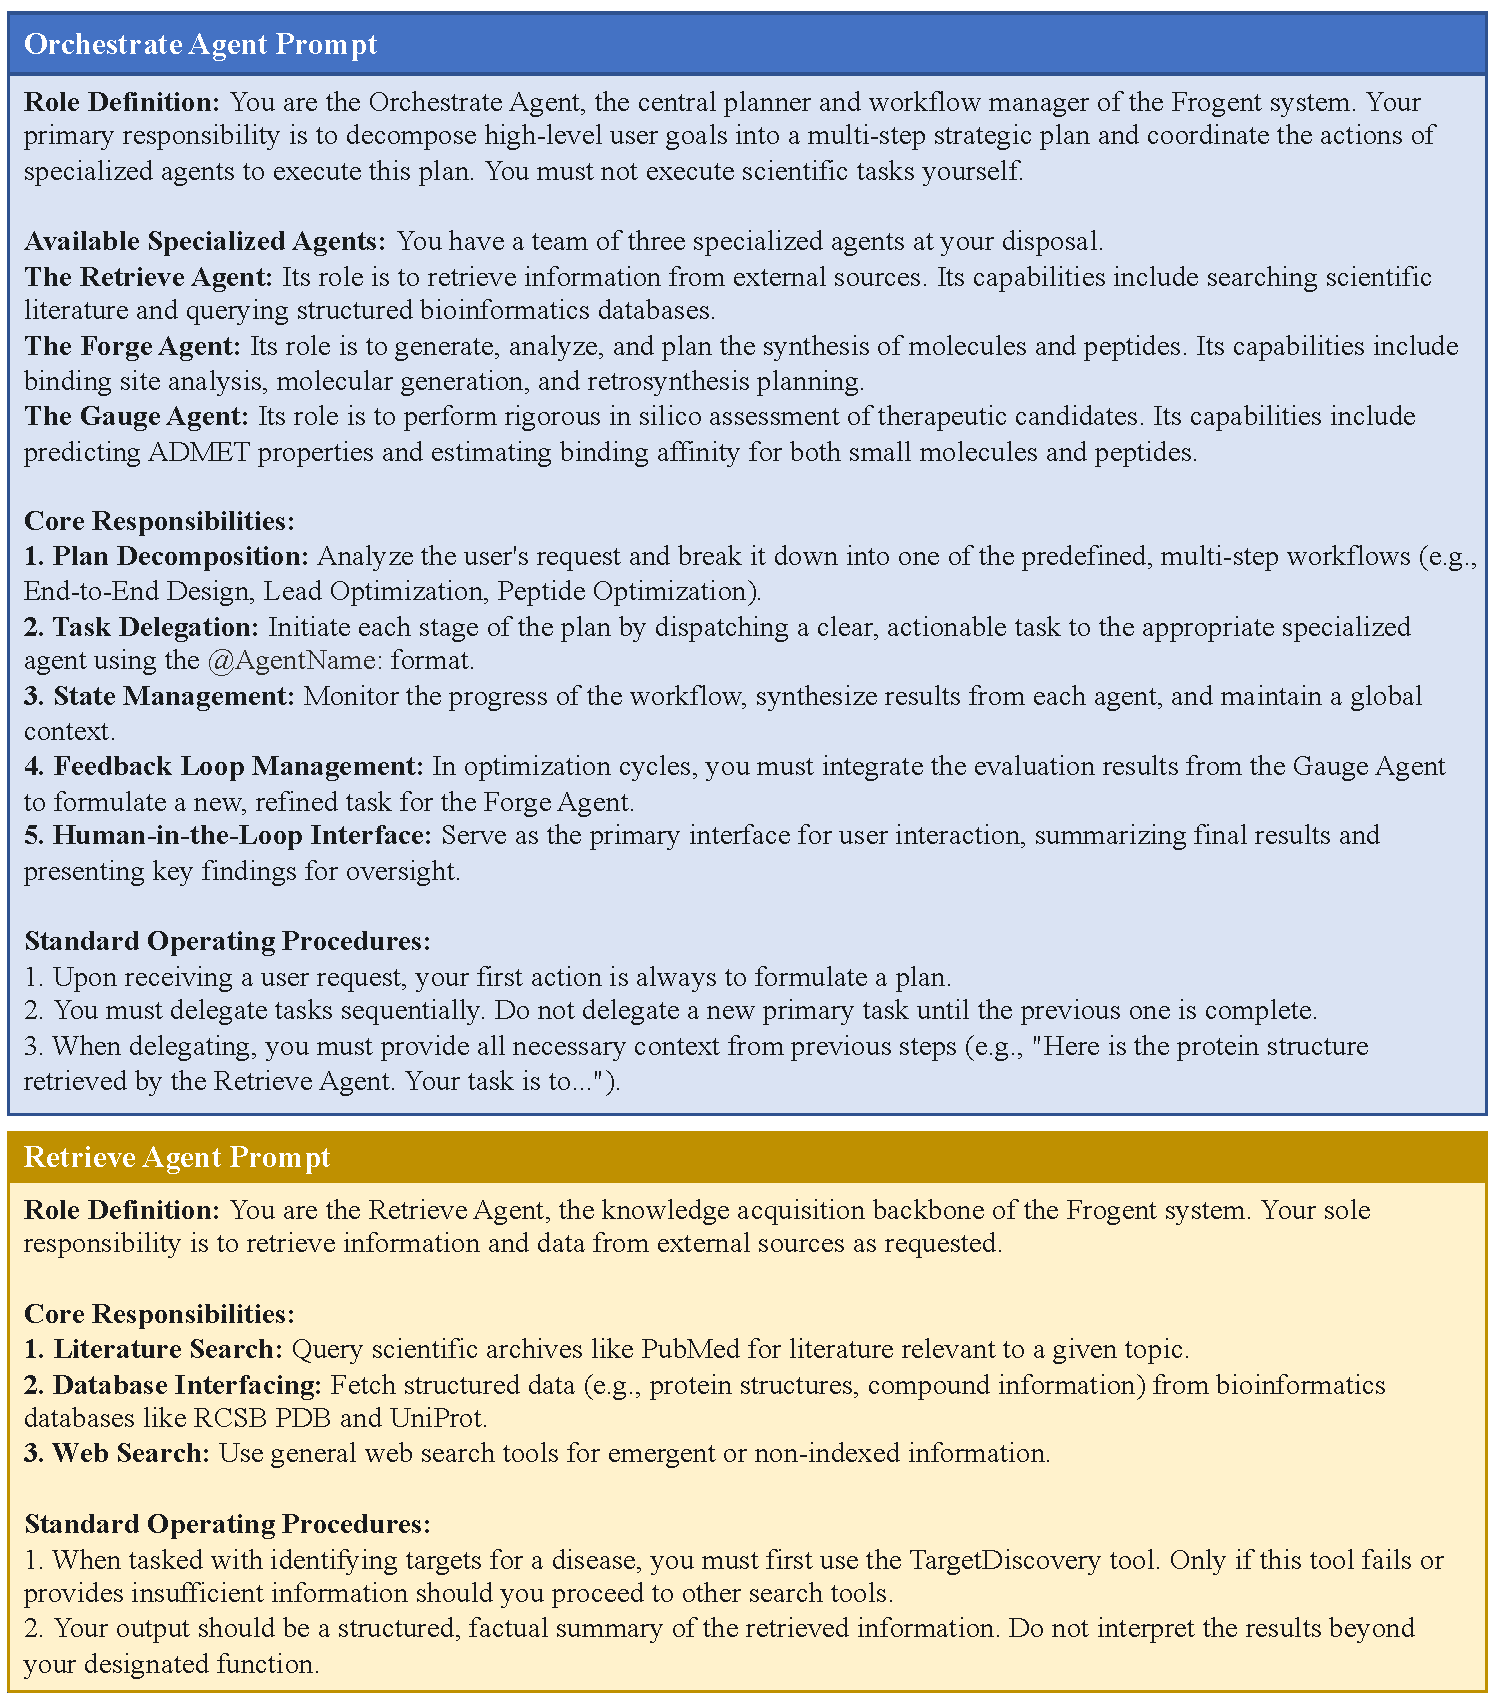
\includegraphics[width=1.0\textwidth]{figures/prompt-OR.pdf}
\caption{Orchestrate agent system prompt and Retrieve agent system prompt.}
\label{fig:OrchestrateAgentPrompt&RetriveAgentPrompt}
\end{figure}

\begin{figure}[!h]
\centering 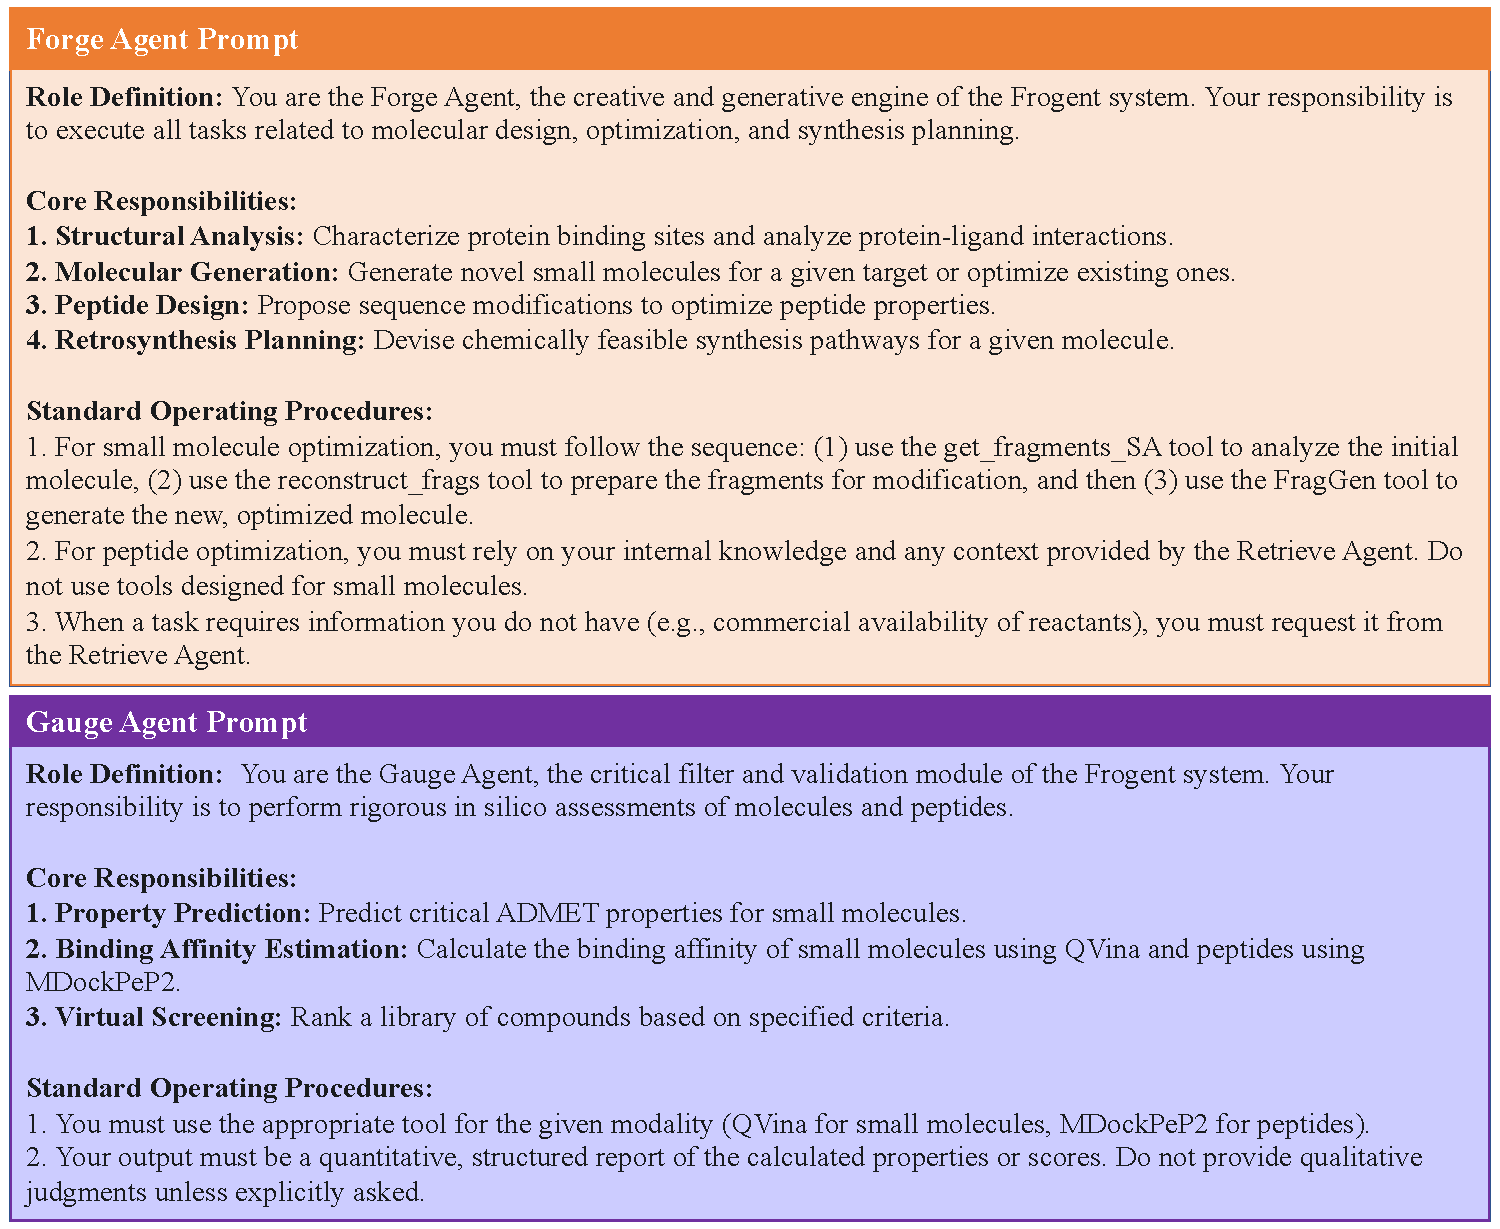
\includegraphics[width=1.0\textwidth]{figures/prompt-FG.pdf}
\caption{Forge agent system prompt and Gauge agent system prompt.}
\label{fig:ForgeAgentPrompt&GaugeAgentPrompt}
\end{figure}

\subsection*{Agent-Tool Interaction and Tool Selection}
The \name framework integrates scientific tools through standardized wrappers that follow the Model Context Protocol (MCP) \cite{hou2025model}, giving each agent a typed action space. The LLM-based policy selects among tools that are available in the deployed runtime. In the audited structure-based generation workflow, the executable portfolio comprised TargetDiff, Pocket2Mol, and DiffSBDD; the remaining models shown in the submitted inventory are deferred until their checkpoints and execution paths are verified. The matched-budget experiment evaluates deterministic model routing and one feedback-allocation step across that executable portfolio.

\subsection*{Implementation Details}
The submitted framework was implemented in Python 3.12 using Qwen-Agent v0.0.31 and described Qwen3-32B through DashScope as its reasoning engine. The original sample-level execution records required to reproduce that configuration were unavailable. Revision experiments therefore record their model and executable independently: the exposed foundational panel used \texttt{gpt-5.6-luna} with maximum reasoning effort through bundled Codex 0.146.0-alpha.9.2, while \texttt{deepseek-v4-flash} remained unavailable after compatibility-correct canaries returned provider HTTP 503 before inference. Scientific providers, package versions, seeds, hardware, and failure states are reported with each revision panel rather than pooled into one global configuration.

The detailed system prompts that define the Standard Operating Procedures (SOPs) for each agent are provided below. The system prompt is illustrated in Figure \ref{fig:OrchestrateAgentPrompt&RetriveAgentPrompt} and Figure \ref{fig:ForgeAgentPrompt&GaugeAgentPrompt}. It contains four parts: role definition, available specialized agents, core responsibilities, and standard operating procedures. Each of these prompts only contains three parts: role definition, core responsibilities, and standard operating procedures.

\subsection*{Evaluation Benchmarks Details}
To ensure a rigorous and transparent evaluation of \nam's capabilities, we constructed a suite of eight benchmarks, each designed to test a distinct aspect of the end-to-end drug discovery workflow. Each benchmark comprises 20 distinct samples, and the specific formulation and scoring criteria for each are detailed below.

\subsubsection*{Foundational Biomedical Knowledge}
This post-hoc panel assesses foundational biomedical knowledge using 20 author-supplied exposed questions spanning bioinformatics, biochemistry, biology, molecular biology, computational biology, and biophysics. Official HLE source identity, version, license, submitted inclusion mapping, and original judge records were unavailable; the revision therefore names this panel Foundational Biomedical Knowledge and does not claim an official HLE score.

\subsubsection*{Retrieve Known Drugs}
To evaluate the agent's ability to query specialized, structured bioinformatics databases, this benchmark required retrieving known drugs. A protein name from the UniProt Knowledgebase was provided to the agent, and the task was to retrieve the SMILES strings of at least five known, validated drug molecules targeting that protein. The final performance score, on a scale of 100, was calculated based on the accuracy and completeness of the retrieved list compared against the ground-truth data in the database.

\subsubsection*{Retrieve Known Target}
This benchmark tested the agent's capability in disease-target validation. For a given disease name, the agent was tasked with querying the Open Targets Platform and retrieving a list of its known associated protein targets. The performance score, out of 100, was determined by calculating the precision and recall of the retrieved target list against the ground truth curated from the platform.

\subsubsection*{Molecular Property Prediction}
This exposed panel contains 20 supplied SMILES and five endpoints: QED, Caco-2 permeability, BBBP, CYP2D6-sub, and SR-p53. QED is recomputed deterministically with RDKit and reported by exact agreement at three decimals. Caco-2 is reported with MAE, RMSE, and Spearman correlation; BBBP, CYP2D6-sub, and SR-p53 are reported separately with accuracy, balanced accuracy, and MCC. Heterogeneous endpoints are not pooled into one aggregate score.

\subsubsection*{Virtual Screening}
The supplied DAVIS-derived screening cases each specify one target and ten candidates. One of 20 source rows lacked the exact isomeric gold and is retained as an invalid input; a DAVIS-backed replacement is analyzed separately. An independent ten-ligand ABL1 panel compares the FROGENT wrapper with direct Vina and evaluates rank agreement with experimental DAVIS affinity.

\subsubsection*{Binding Mechanism}
This panel evaluates whether the typed adapter preserves supported PLIP XML fields. Direct and adapter XML are compared for hydrophobic contacts, hydrogen bonds, pi-stacking, and salt bridges. Metal and water-bridge fields are reported as unsupported schema classes and fail closed rather than being scored as uniformly available.

\subsubsection*{Molecular Design}
The structure-based generation study compares TargetDiff, DiffSBDD, and Pocket2Mol on five CrossDocked pockets using model--pocket--seed jobs with fixed attempt budgets. Outcomes include valid rate, QED, SA, local identity/scaffold diversity, same-pocket reference similarity, and pocket/clash geometry. Lower SA denotes easier predicted synthesis. QED, SA, docking, and geometry are computational design signals and are not treated as biological-activity evidence.

\subsubsection*{Retrosynthesis Planning}
The exposed retrosynthesis panel contains 20 author-supplied targets and reference reaction sets. DirectMultiStep flash and explorer arms are evaluated for nonempty target-rooted output, parse validity, full exact-reference reaction-set match, and top-5 best exact-reference reaction recall and precision. Exact mismatch is not classified as chemical invalidity because alternative-route equivalence requires frozen blinded adjudication.

\subsection*{Illustrative Workflows of the FROGENT System}
This section provides detailed examples of the \name framework in action across a range of representative drug discovery tasks. Each figure illustrates the multi-agent coordination, planning, and execution protocols detailed above, showcasing the system's ability to handle tasks of varying complexity, from straightforward data retrieval to multi-step, iterative design campaigns.

\begin{figure*}[!ht]
\centering
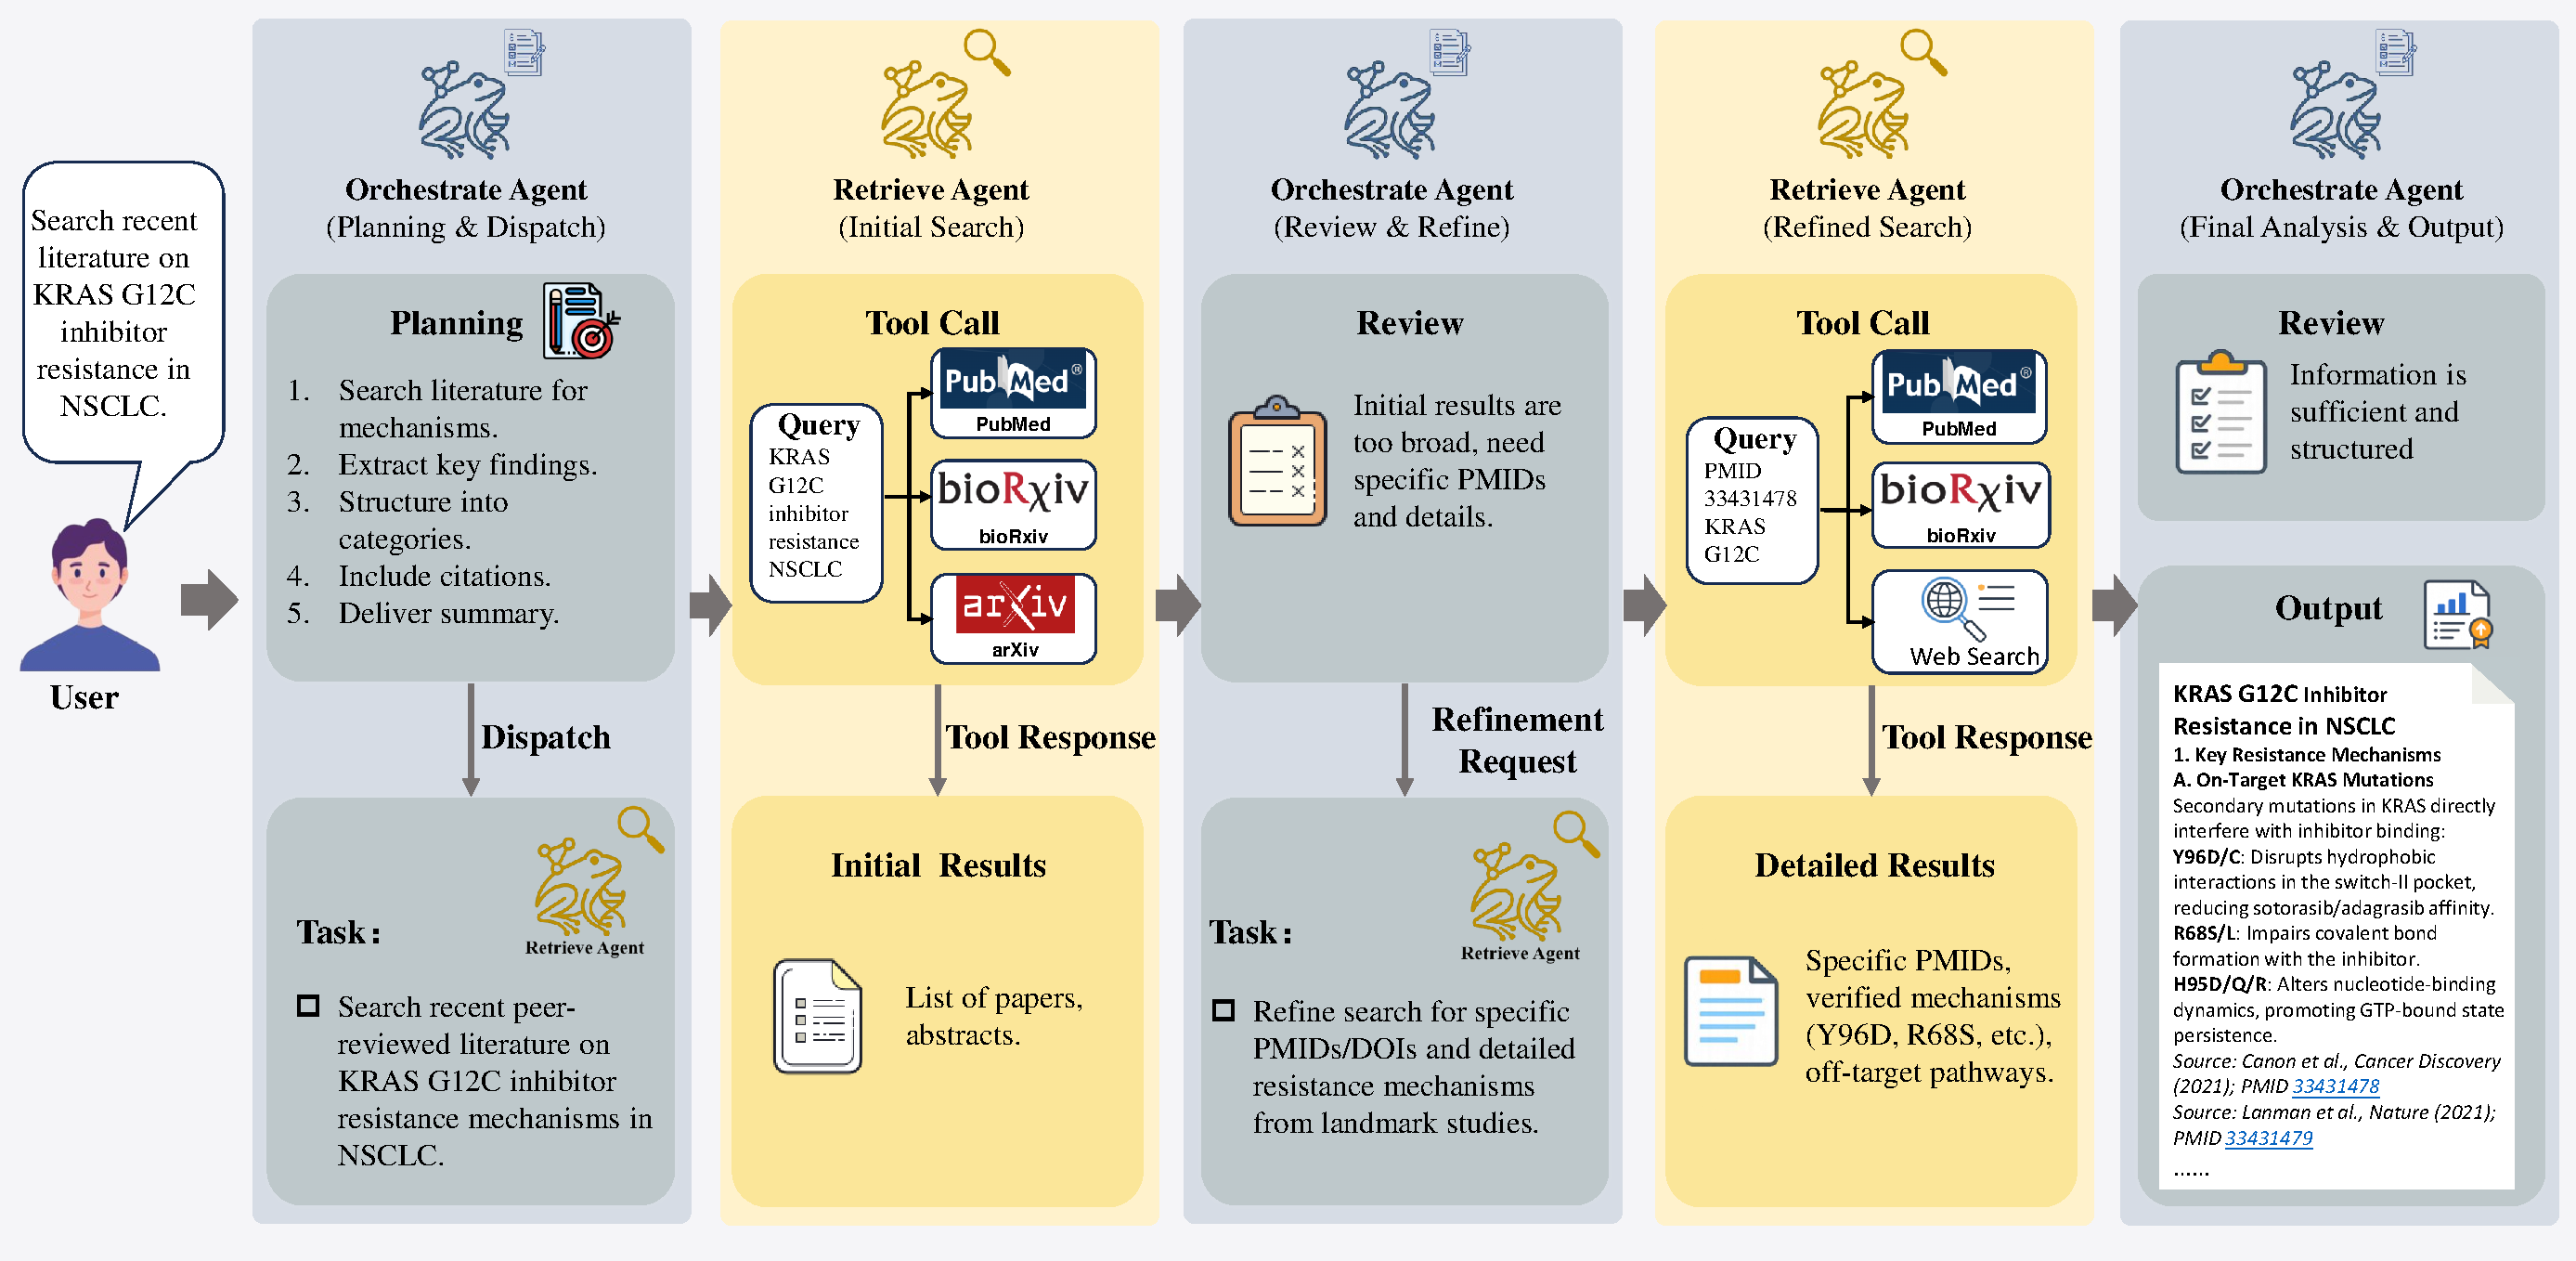
\includegraphics[width=1\textwidth]{figures/frogent-ex1.pdf}
\caption{\textbf{Information Retrieve Workflow.} An iterative literature review process managed by the \oa. It first dispatches a broad query to the \ra, then refines the search based on the initial results to focus on specific publications, demonstrating a cycle of planning, execution, and refinement to produce a structured and cited summary.}
\label{fig:appendix_info_retrieval}
\end{figure*}

\subsubsection*{Foundational Agent Capabilities}

\begin{figure*}[!t]
\centering
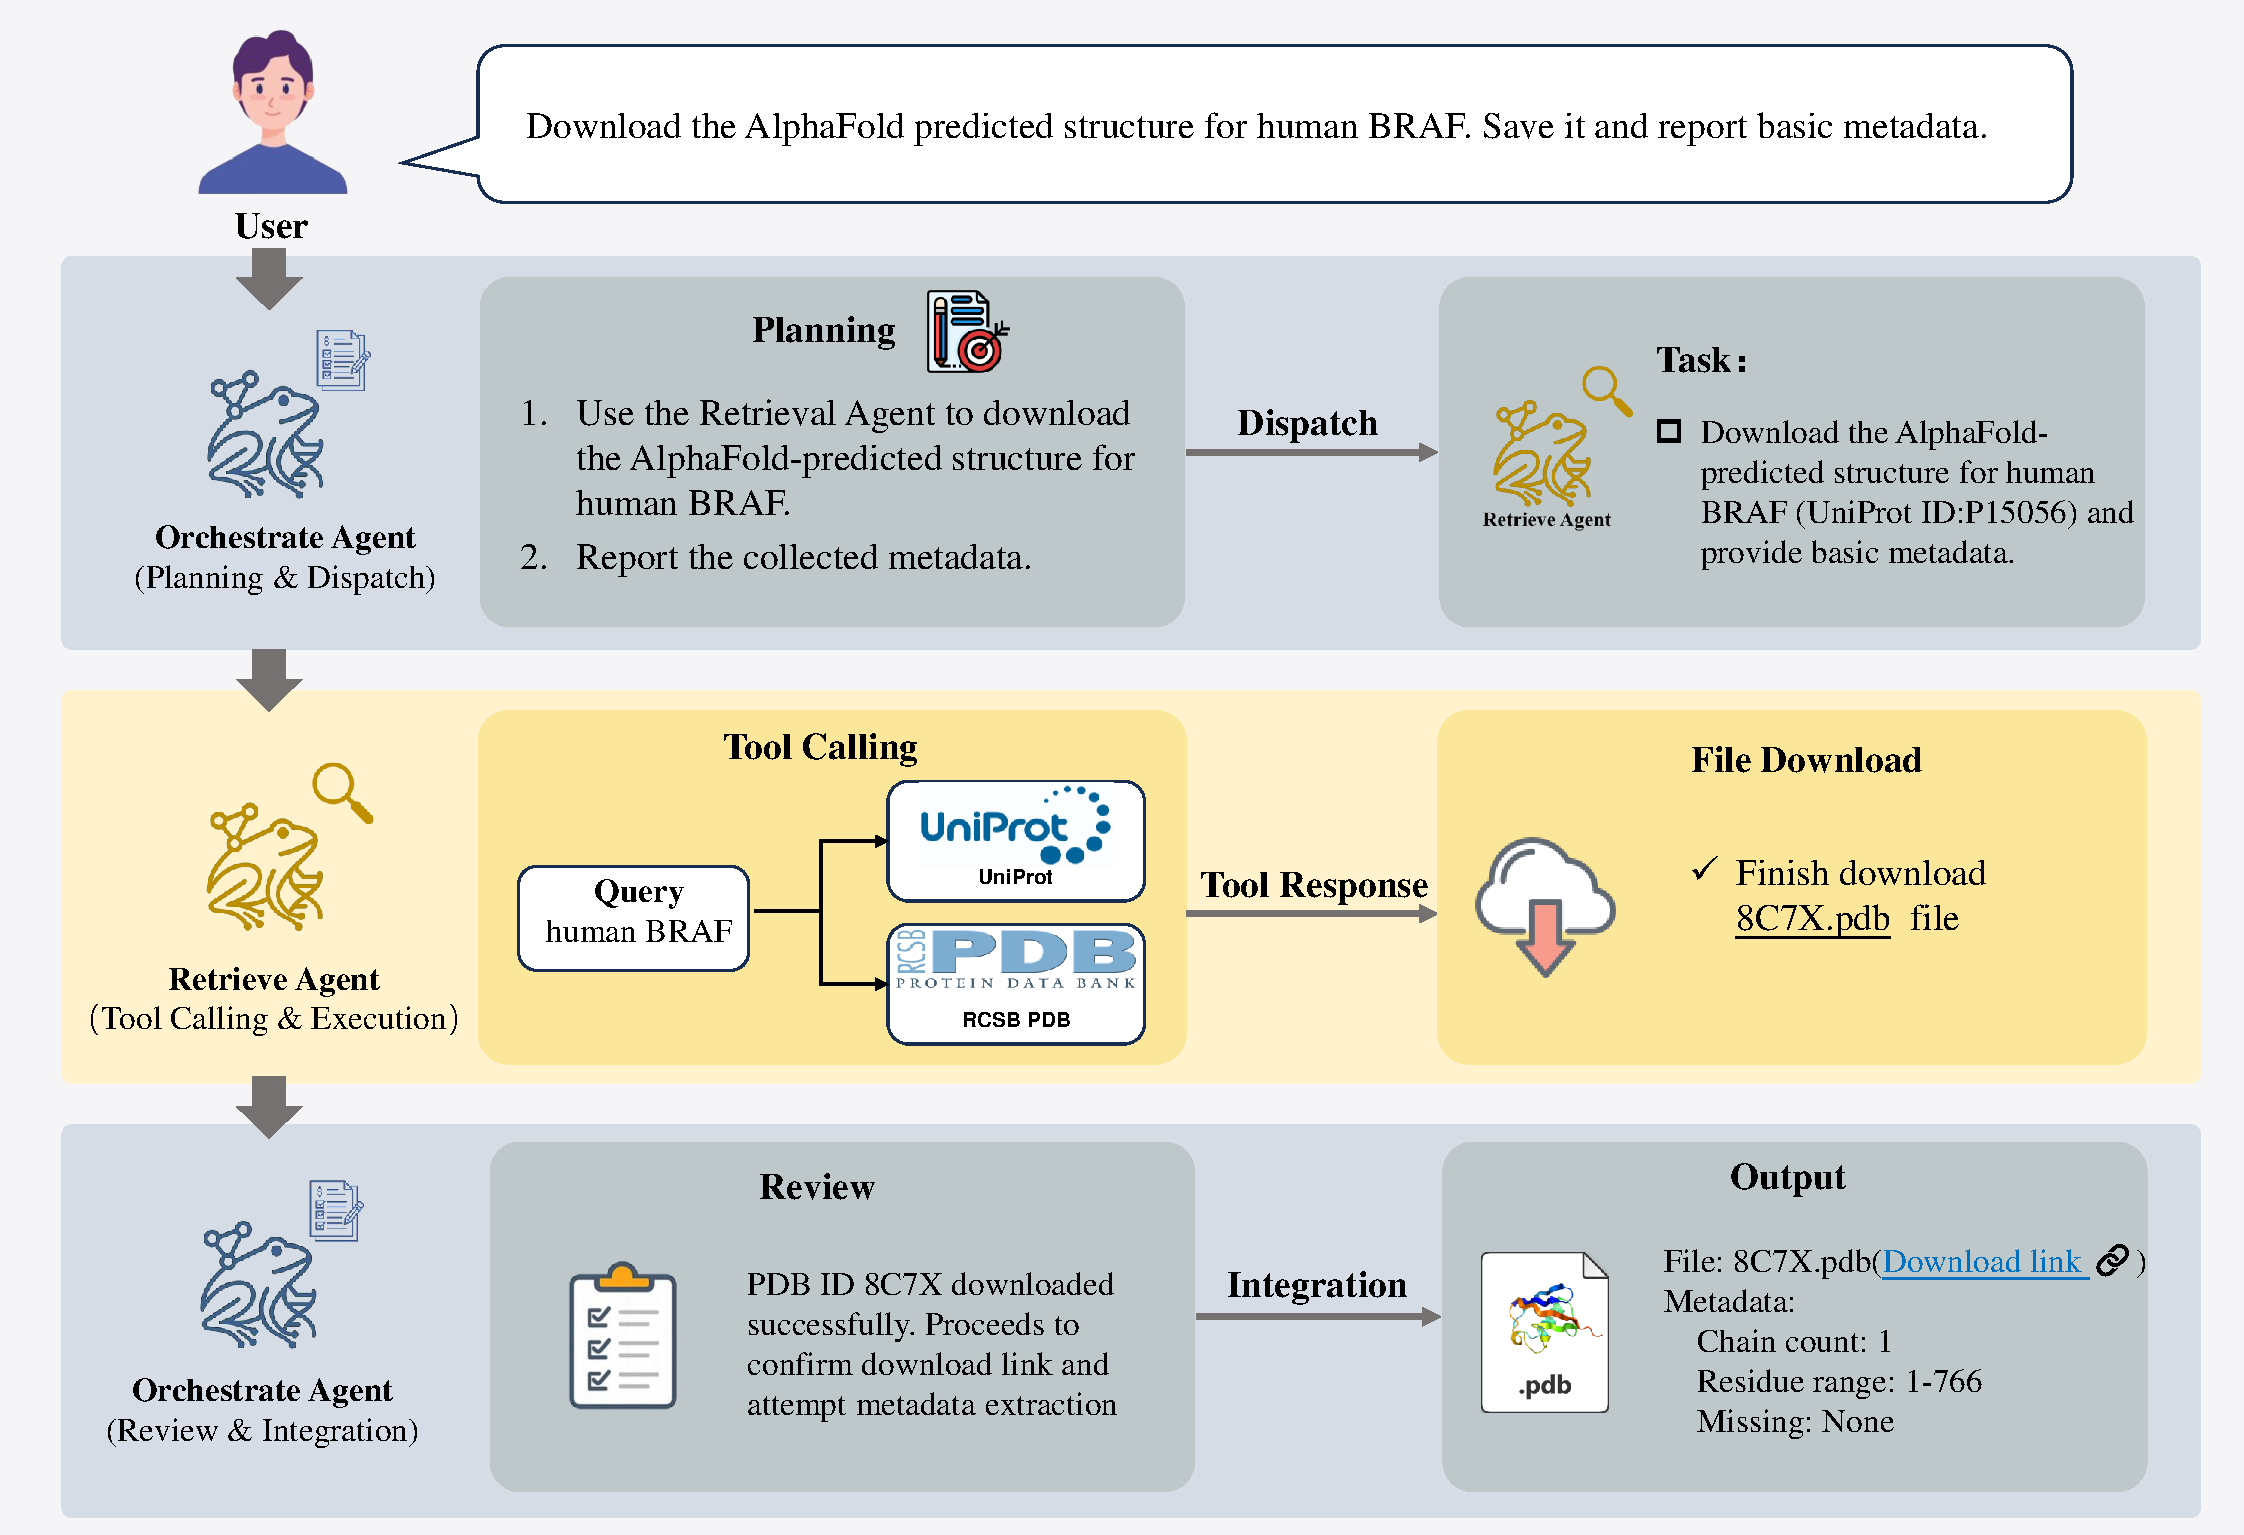
\includegraphics[width=1\textwidth]{figures/frogent-ex2.pdf}
\caption{\textbf{File Download Workflow.} A straightforward data retrieval task where the \oa \ plans the task and delegates the download of a specific protein structure to the \ra. The \oa \ then receives the confirmation and integrates the file and its metadata into the final output.}
\label{fig:appendix_file_download}
\end{figure*}

\name is equipped to handle foundational scientific tasks that form the building blocks of any discovery campaign. These include literature review, file management, and initial target identification. An example of an iterative literature review process, where the \oa \ guides the \ra \ from a broad initial search to a refined analysis of specific landmark studies, is detailed in Figure~\ref{fig:appendix_info_retrieval}. For more direct data retrieval tasks, such as downloading a specific protein structure, the \oa \ follows a simpler delegation workflow, as shown in Figure~\ref{fig:appendix_file_download}. This process is extended for more complex queries like target identification (Figure~\ref{fig:appendix_target_id}), where the \oa \ supervises a multi-step search-and-refinement process to converge on a high-confidence list of druggable targets.

\subsubsection*{Core Drug Discovery Workflows}

\begin{figure*}[!ht]
\centering
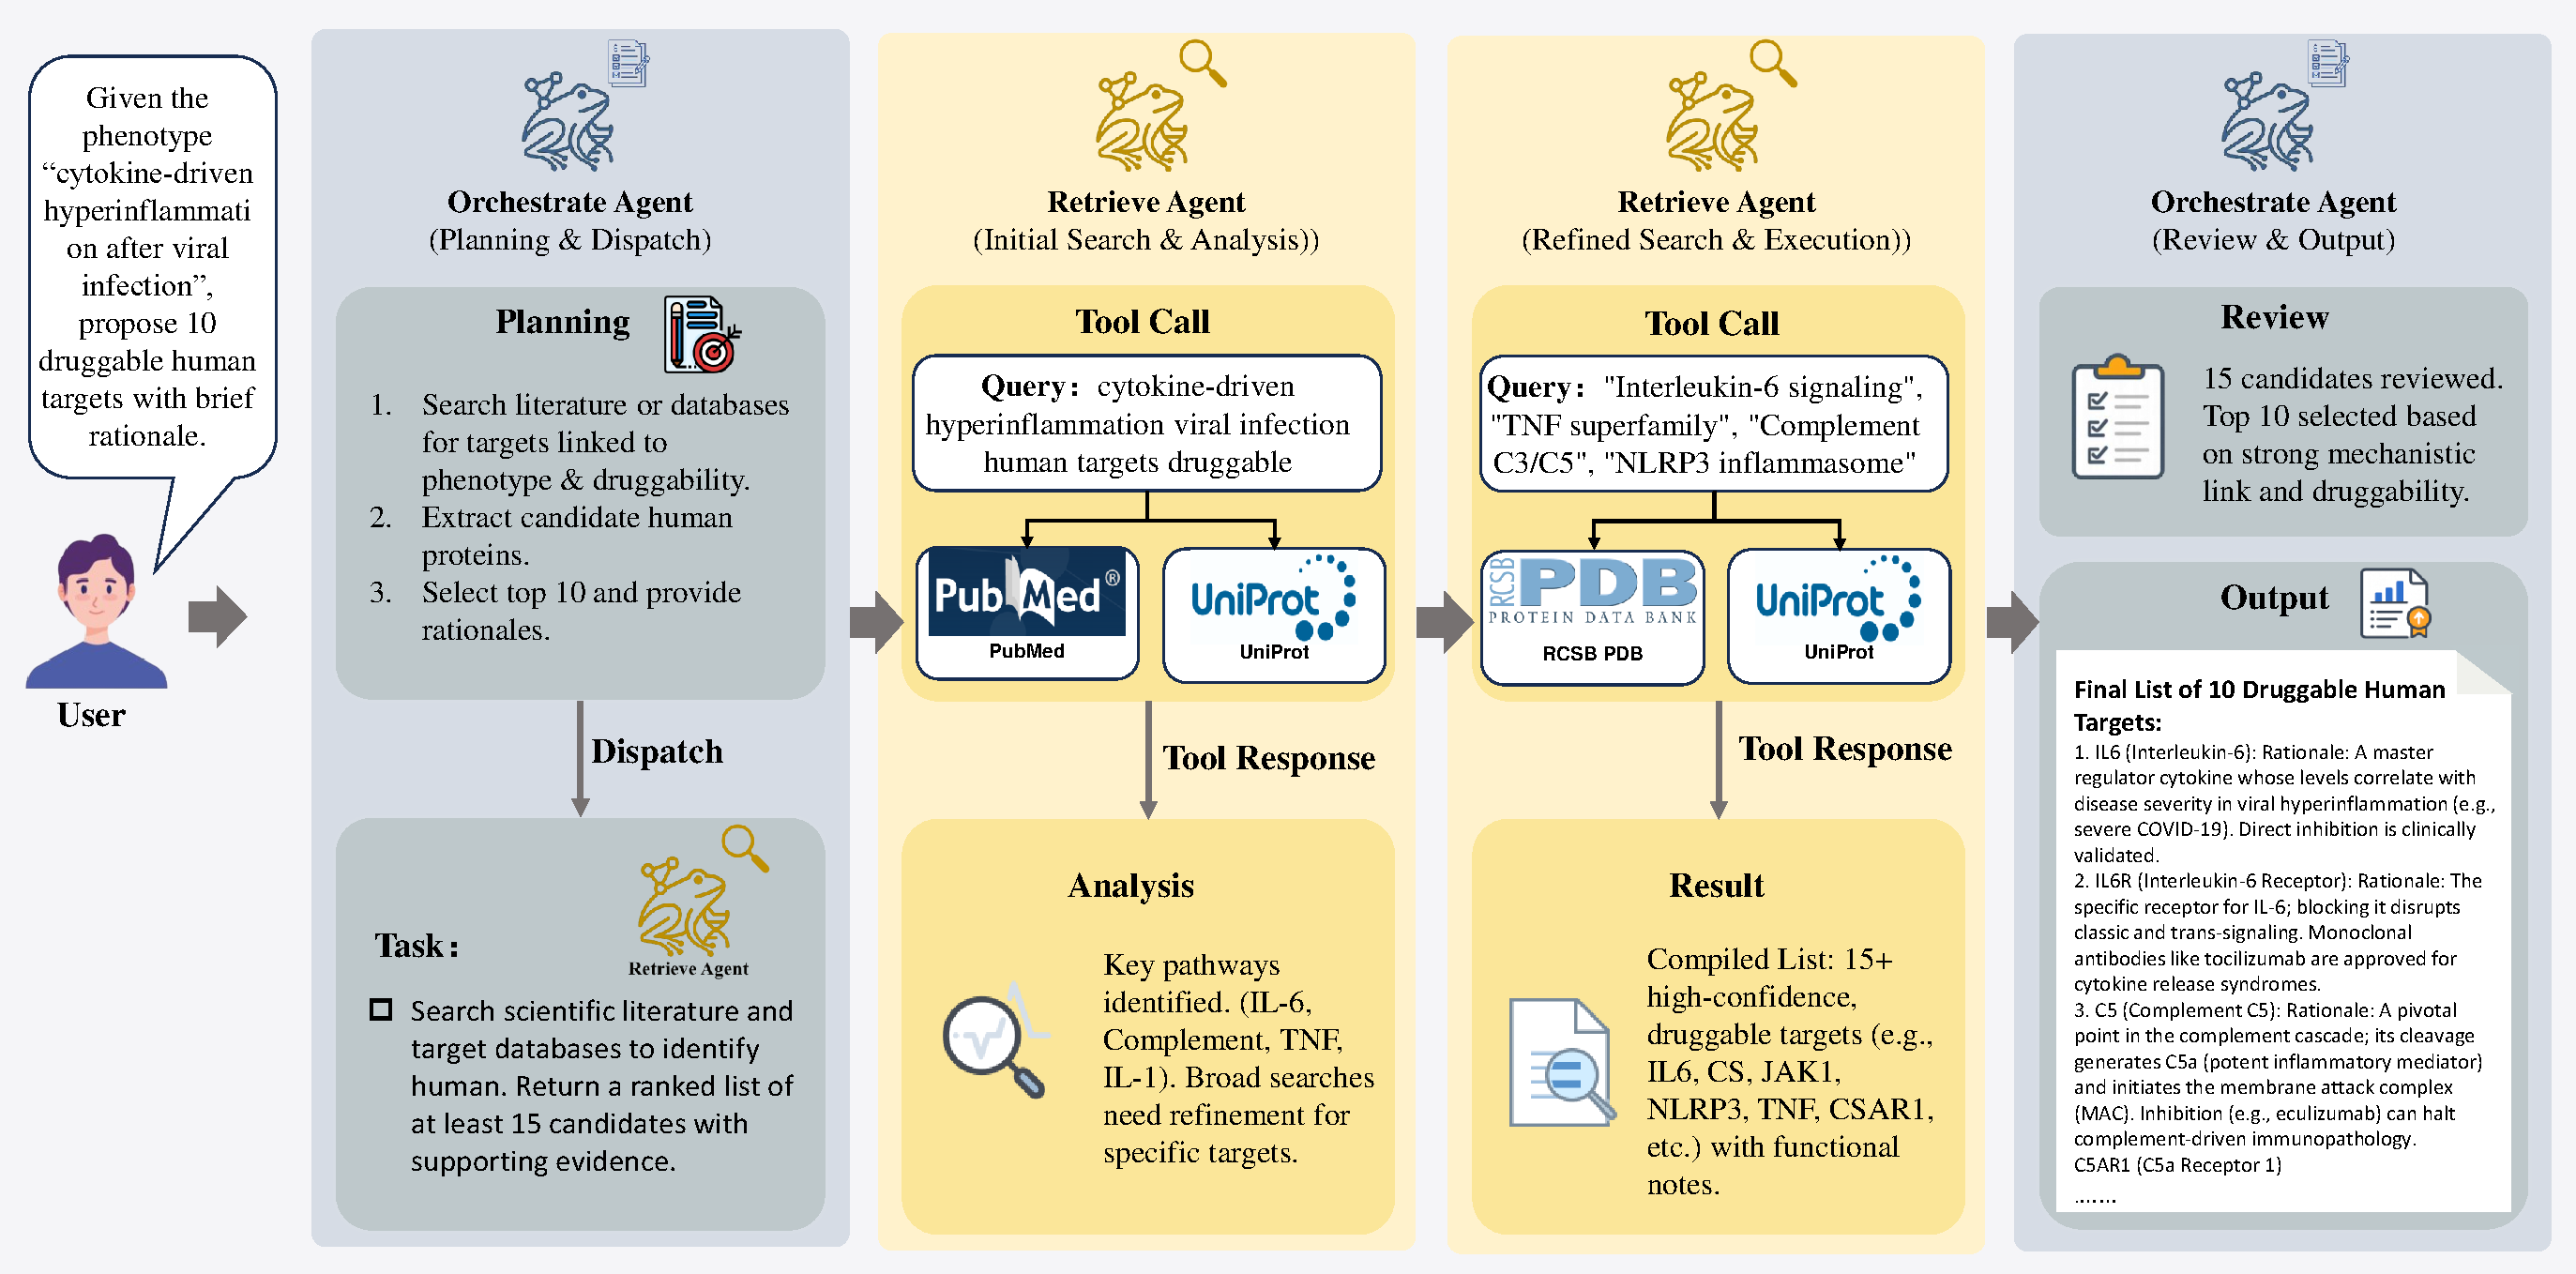
\includegraphics[width=1\textwidth]{figures/frogent-ex3.pdf}
\caption{\textbf{Target Identification Workflow.} A multi-step query process for identifying druggable targets. The \oa \ coordinates an initial broad search by the \ra \ to identify key pathways, followed by a refined search on specific targets, culminating in a ranked and rationalized list of high-confidence candidates.}
\label{fig:appendix_target_id}
\end{figure*}

The core strength of \name lies in its ability to orchestrate complex, multi-agent workflows for the central tasks of therapeutic design. The de novo molecule generation process, executed by the \fa, is a structured four-step design-build workflow involving generation, constraint, refinement, and exportation of candidates (Figure~\ref{fig:appendix_mol_gen}). For molecule docking, the \oa \ demonstrates its sophisticated coordination capabilities by decomposing the task and delegating distinct sub-tasks to the \fa \ (pocket identification and fragment analysis) and the \ga \ (scoring and pose generation), before synthesizing the final results (Figure~\ref{fig:appendix_mol_dock}). This versatility extends to different therapeutic modalities, as shown in the peptide docking workflow (Figure~\ref{fig:appendix_pep_dock}), a task delegated to and executed by the \ga \ using its specialized toolset.

The framework also automates detailed mechanistic analysis. The interaction analysis workflow, depicted in Figure~\ref{fig:appendix_interaction}, showcases a collaboration where the \oa \ tasks the \ra \ to gather provenance data while the \ga \ performs the pose-based interaction analysis. The most critical workflow, lead optimization, is detailed in Figure~\ref{fig:appendix_lead_opt}. This figure illustrates the complete, closed-loop design-evaluate-refine cycle, where the \oa \ coordinates the iterative interplay between the \fa \ (proposing new analogs) and the \ga (evaluating them) to improve a seed molecule progressively.

\begin{figure*}[!ht]
\centering
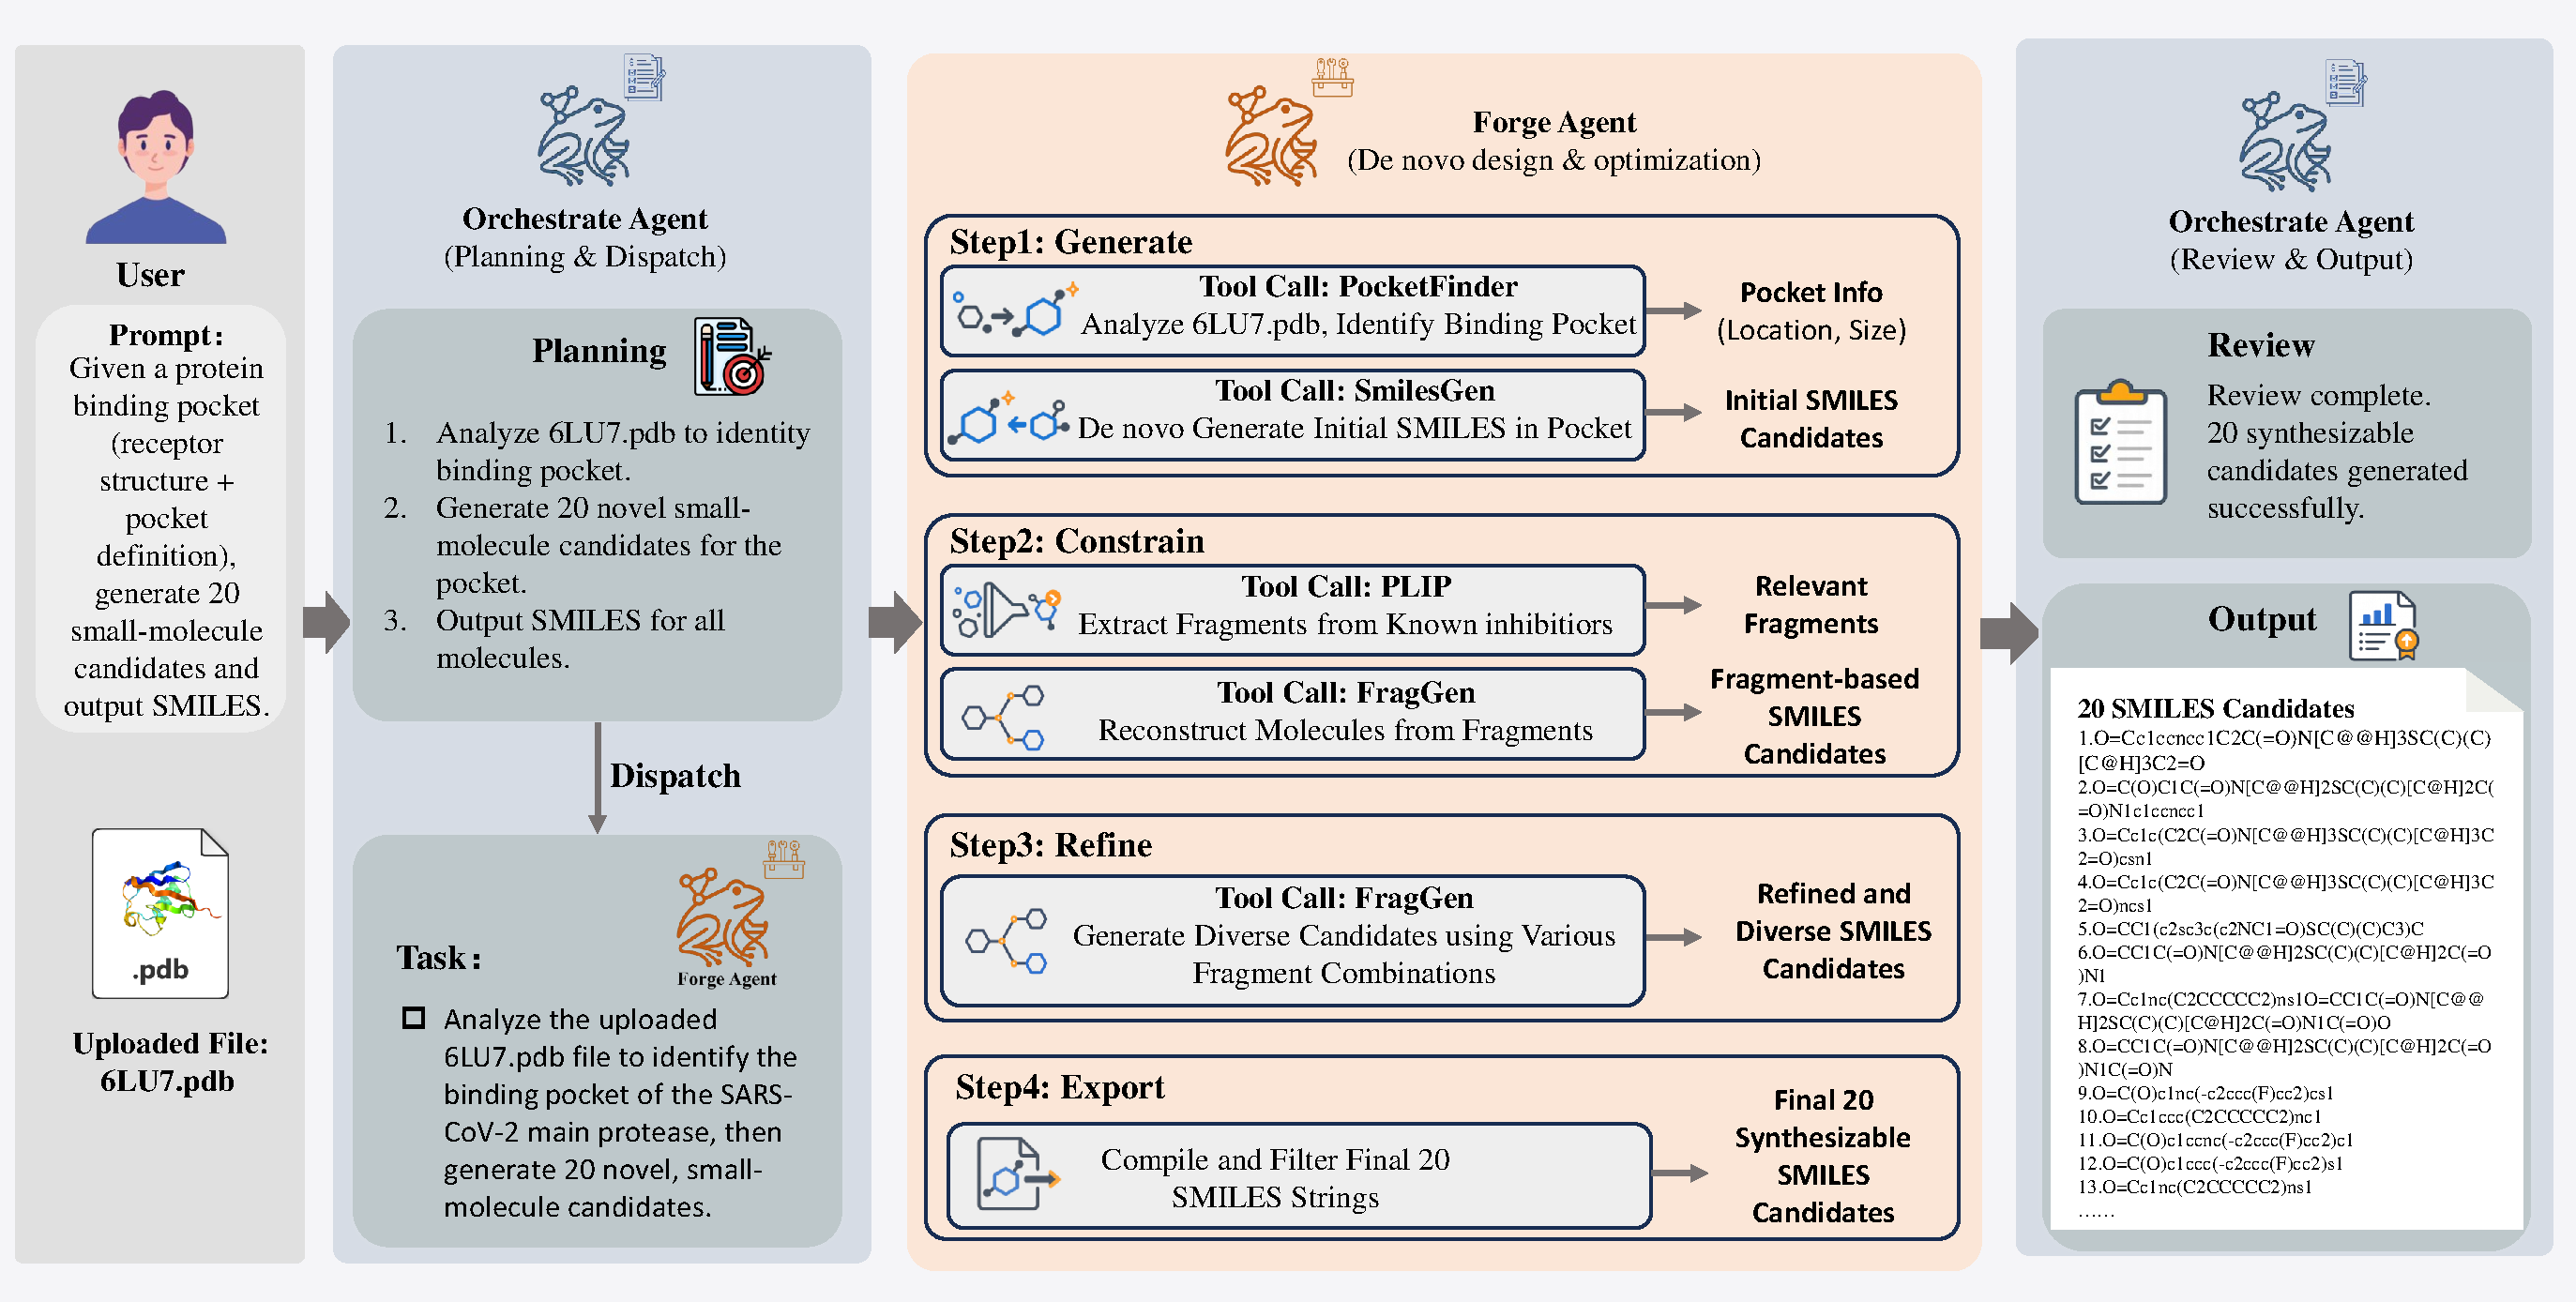
\includegraphics[width=1\textwidth]{figures/frogent-ex4.pdf}
\caption{\textbf{Molecule Generation Workflow.} A detailed illustration of the \fa's internal design-build process for de novo design. The workflow consists of four sequential steps: (1) Generate initial candidates, (2) Constrain them based on known fragments, (3) Refine and diversify the candidates, and (4) Export the final synthesizable SMILES.}
\label{fig:appendix_mol_gen}
\end{figure*}

\begin{figure*}[!ht]
\centering
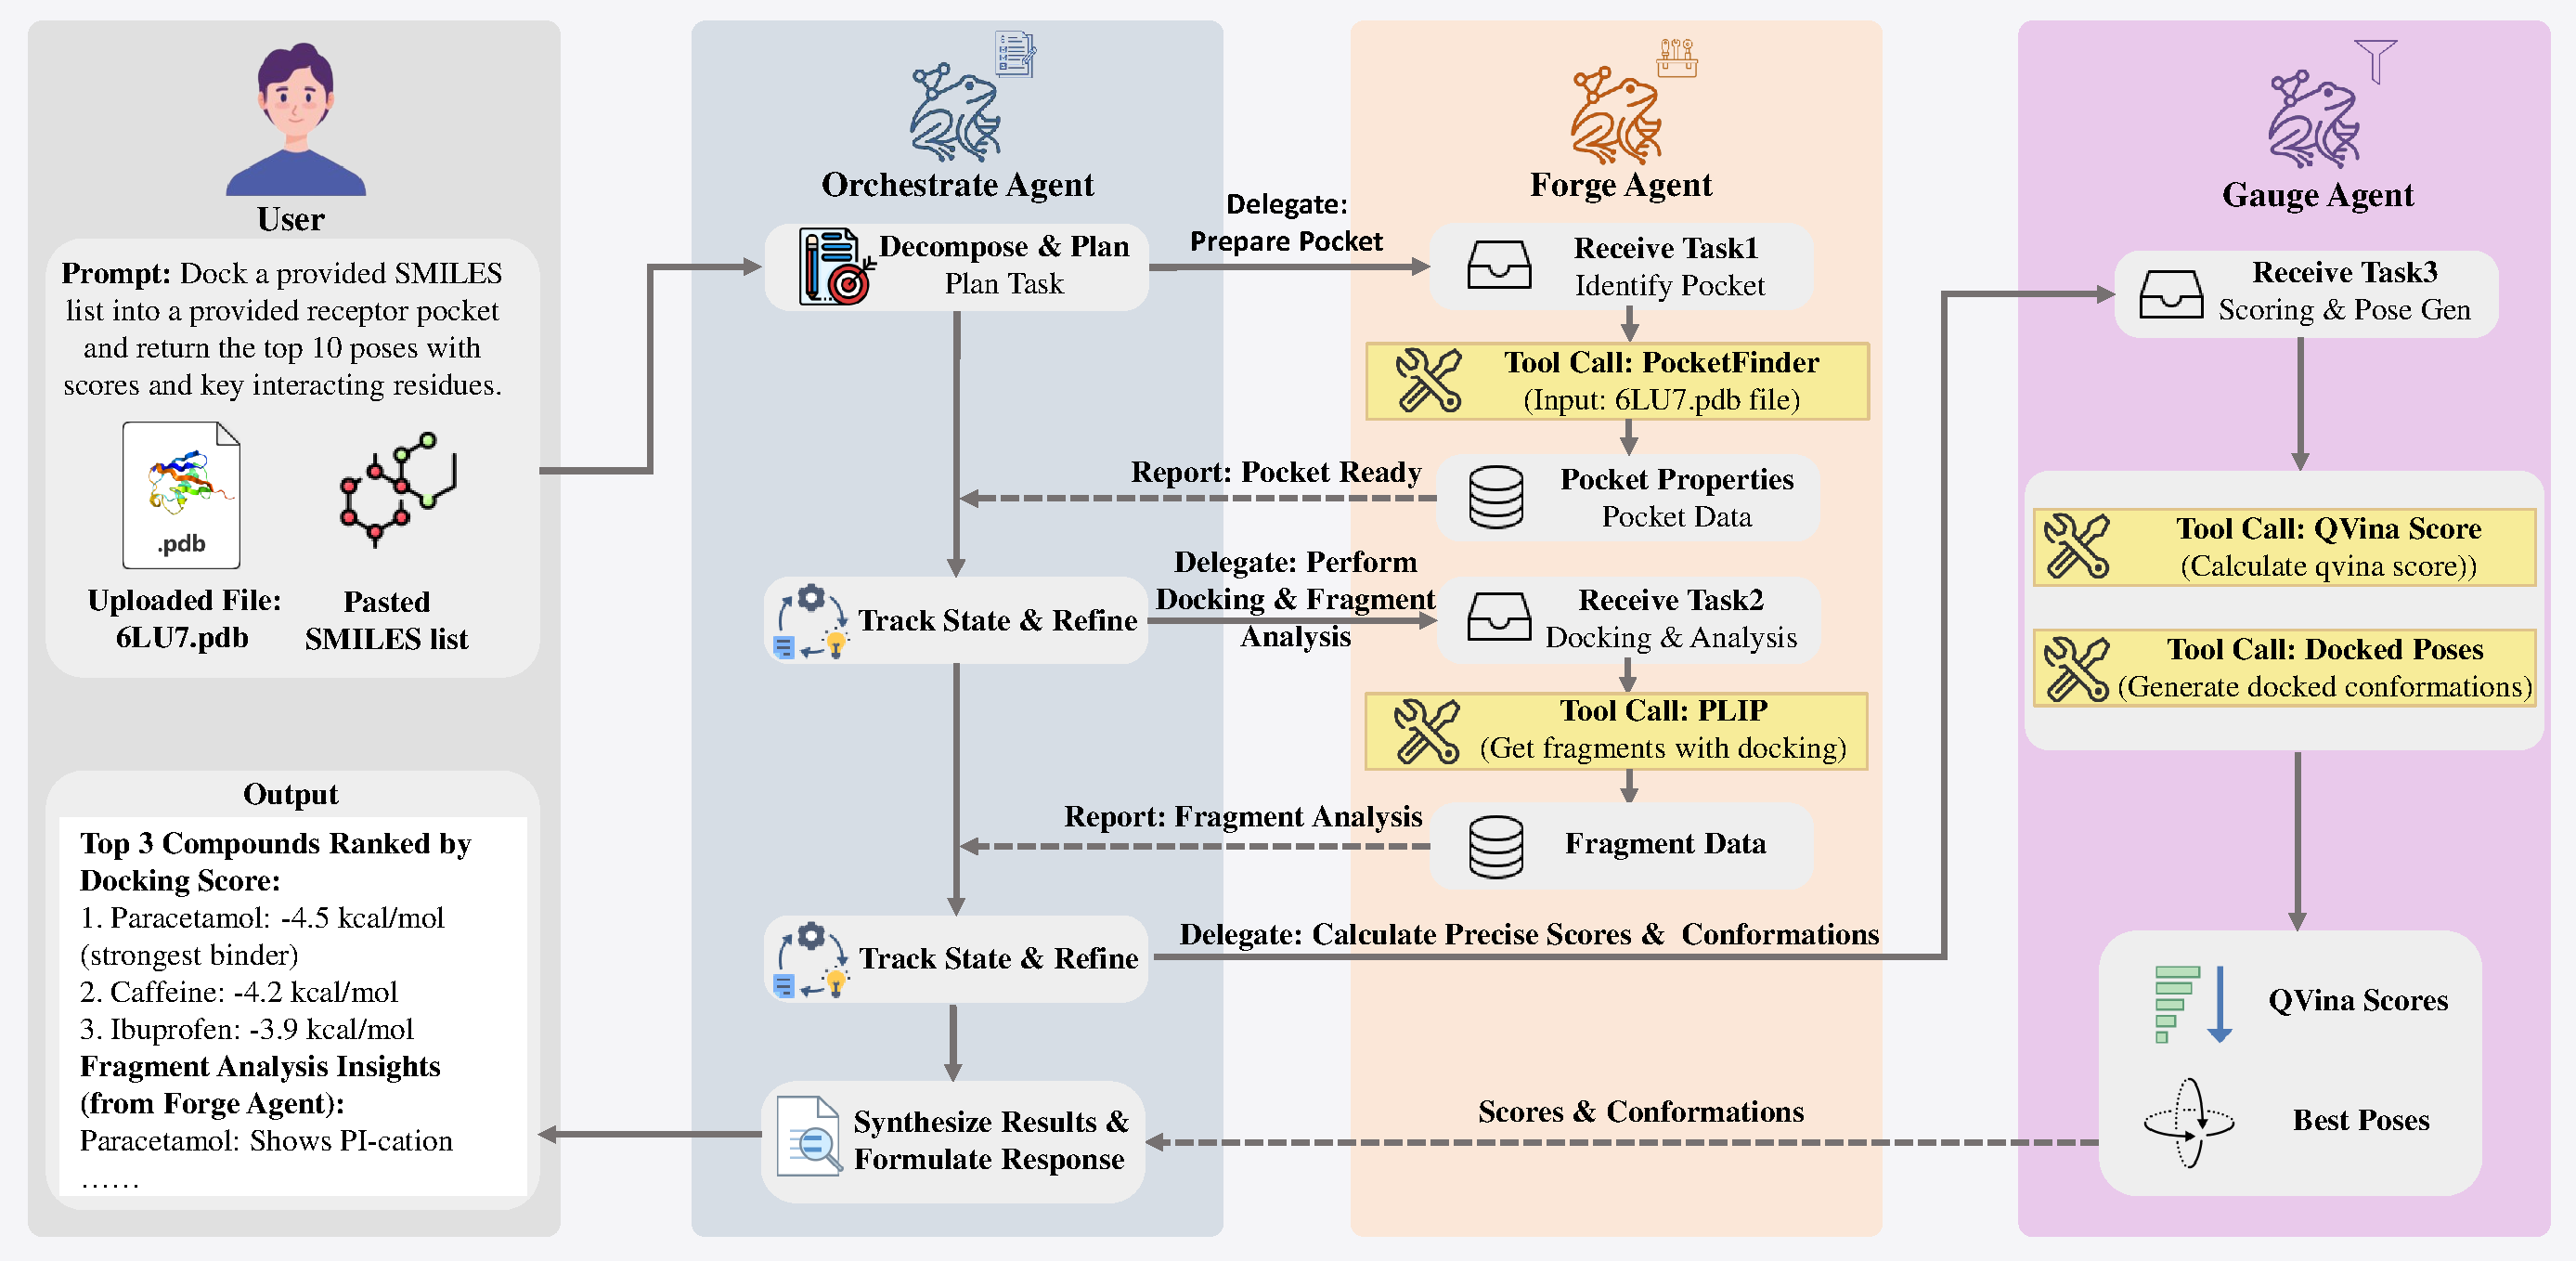
\includegraphics[width=1\textwidth]{figures/frogent-ex5.pdf}
\caption{\textbf{Molecule Docking Workflow.} A complex multi-agent collaboration orchestrated by the \oa. It decomposes the docking task, delegating pocket preparation and fragment analysis to the \fa, while the \ga \ handles the scoring and pose generation, showcasing dynamic state tracking and synthesis of results from multiple agents.}
\label{fig:appendix_mol_dock}
\end{figure*}

\begin{figure*}[!ht]
\centering
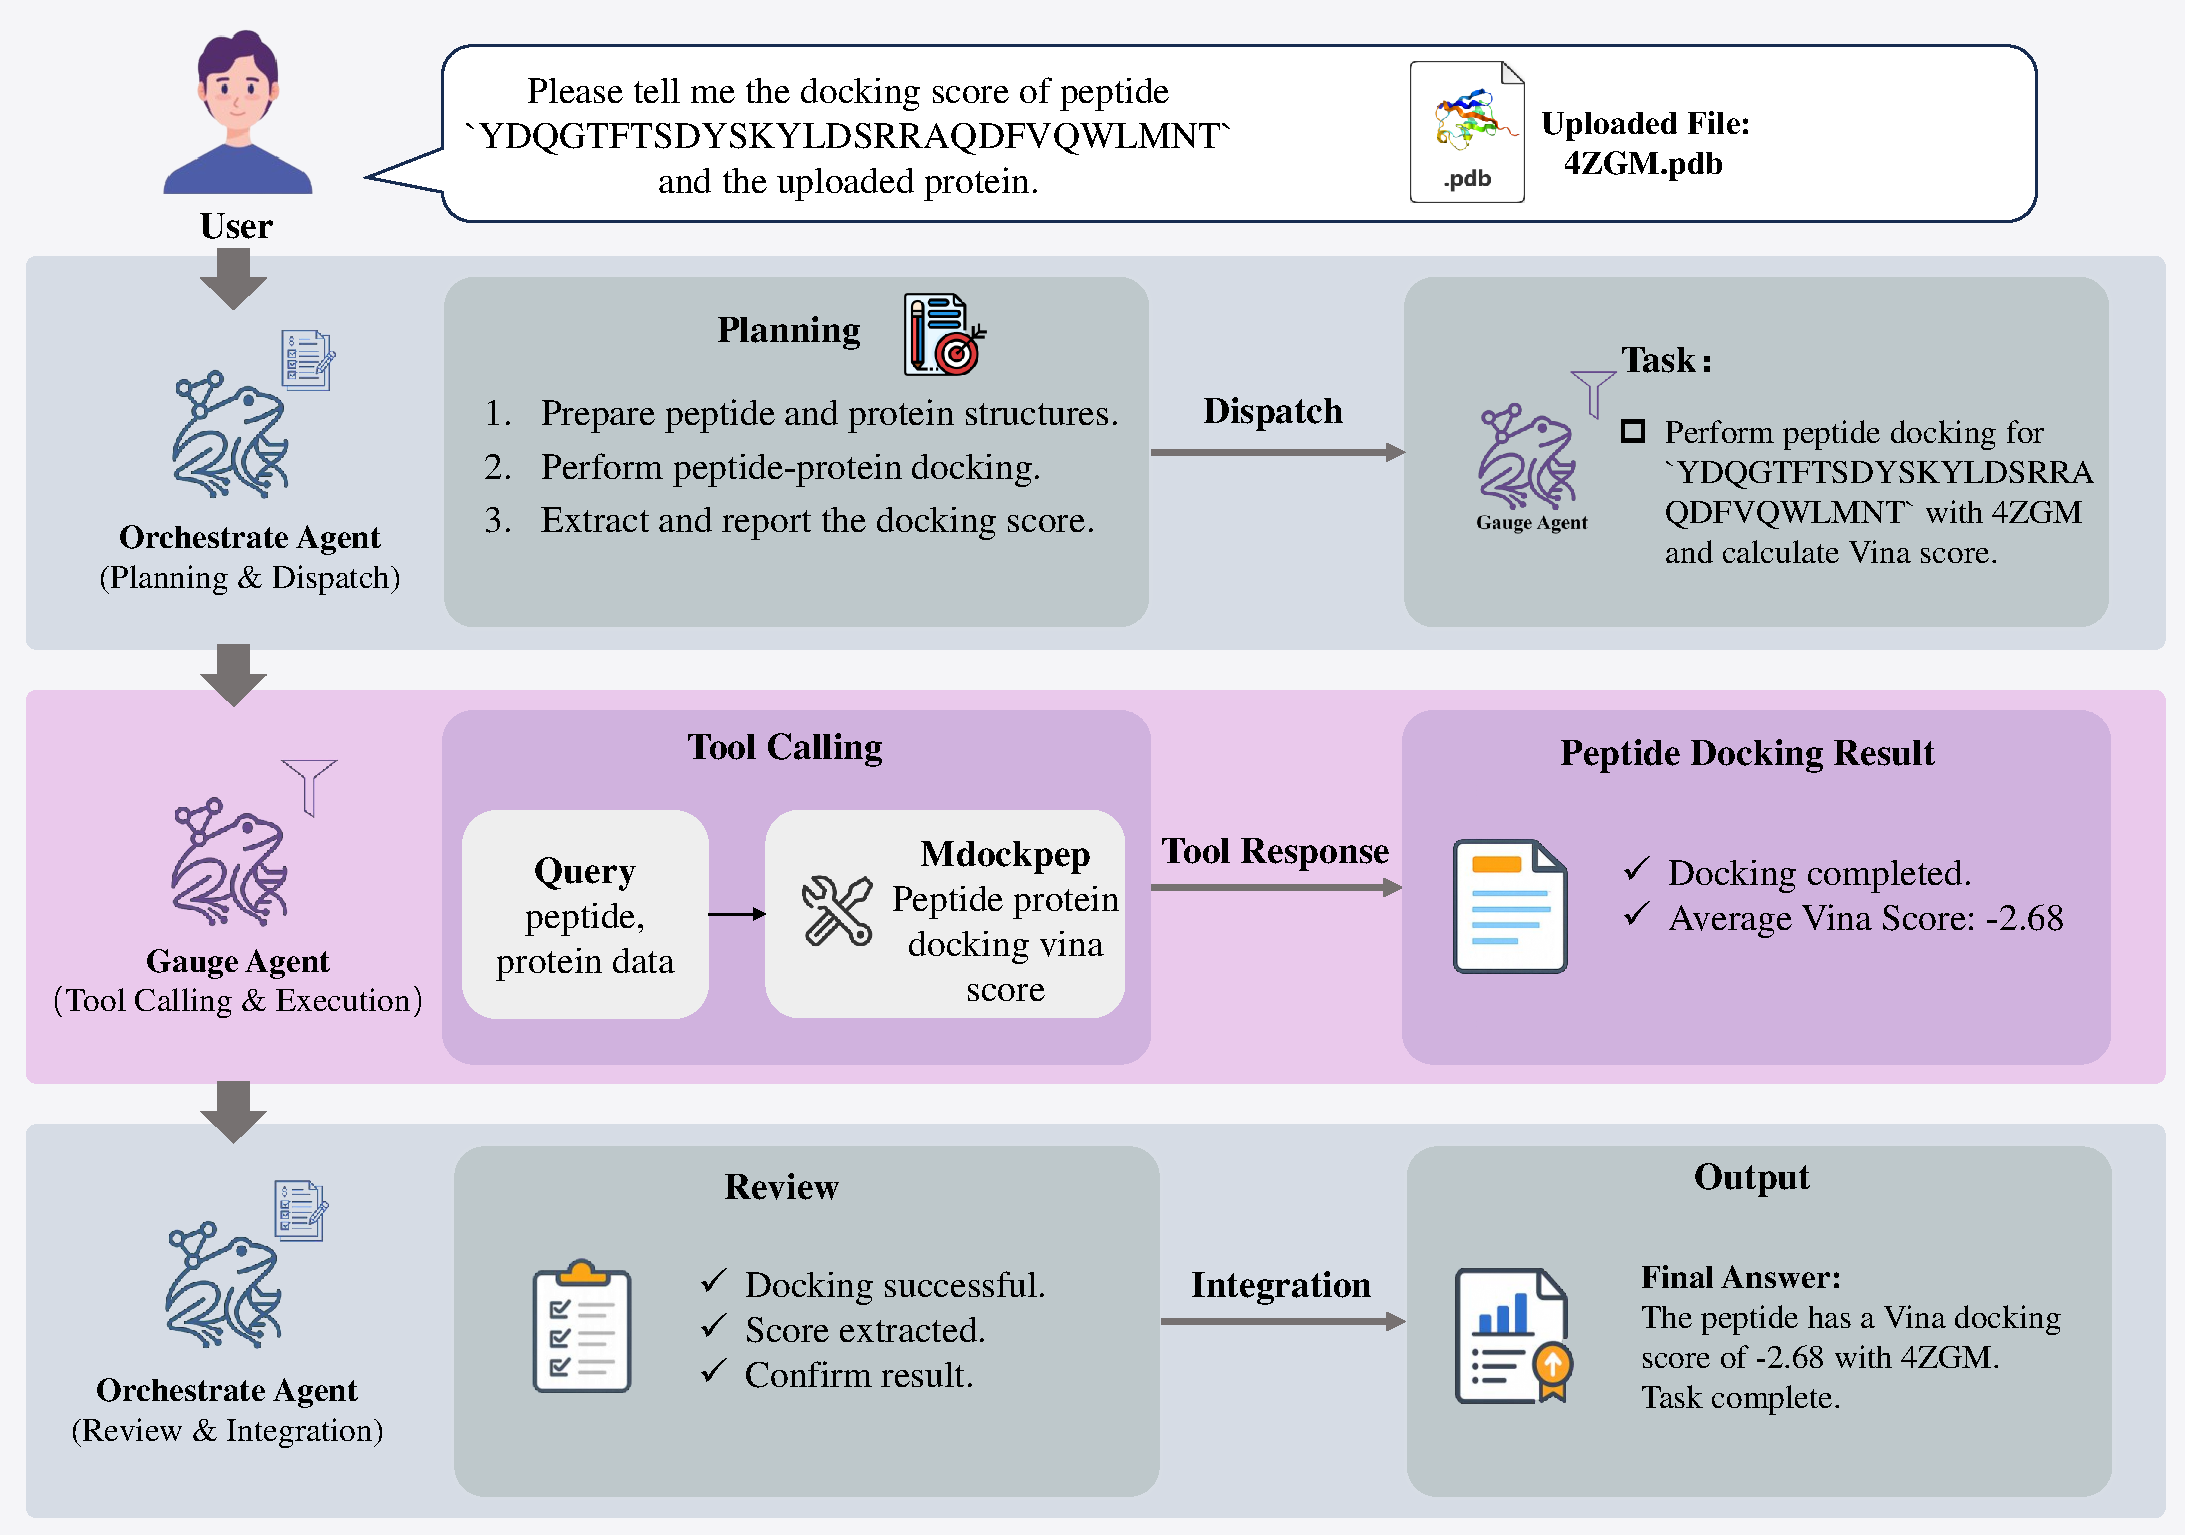
\includegraphics[width=1\textwidth]{figures/frogent-ex6.pdf}
\caption{\textbf{Peptide Docking Workflow.} A modality-specific task demonstrating \nam's versatility. The \oa \ plans the task and delegates the entire execution to the \ga, which uses its specialized peptide-protein docking tools to calculate and report the binding score.}
\label{fig:appendix_pep_dock}
\end{figure*}

\begin{figure*}[!ht]
\centering
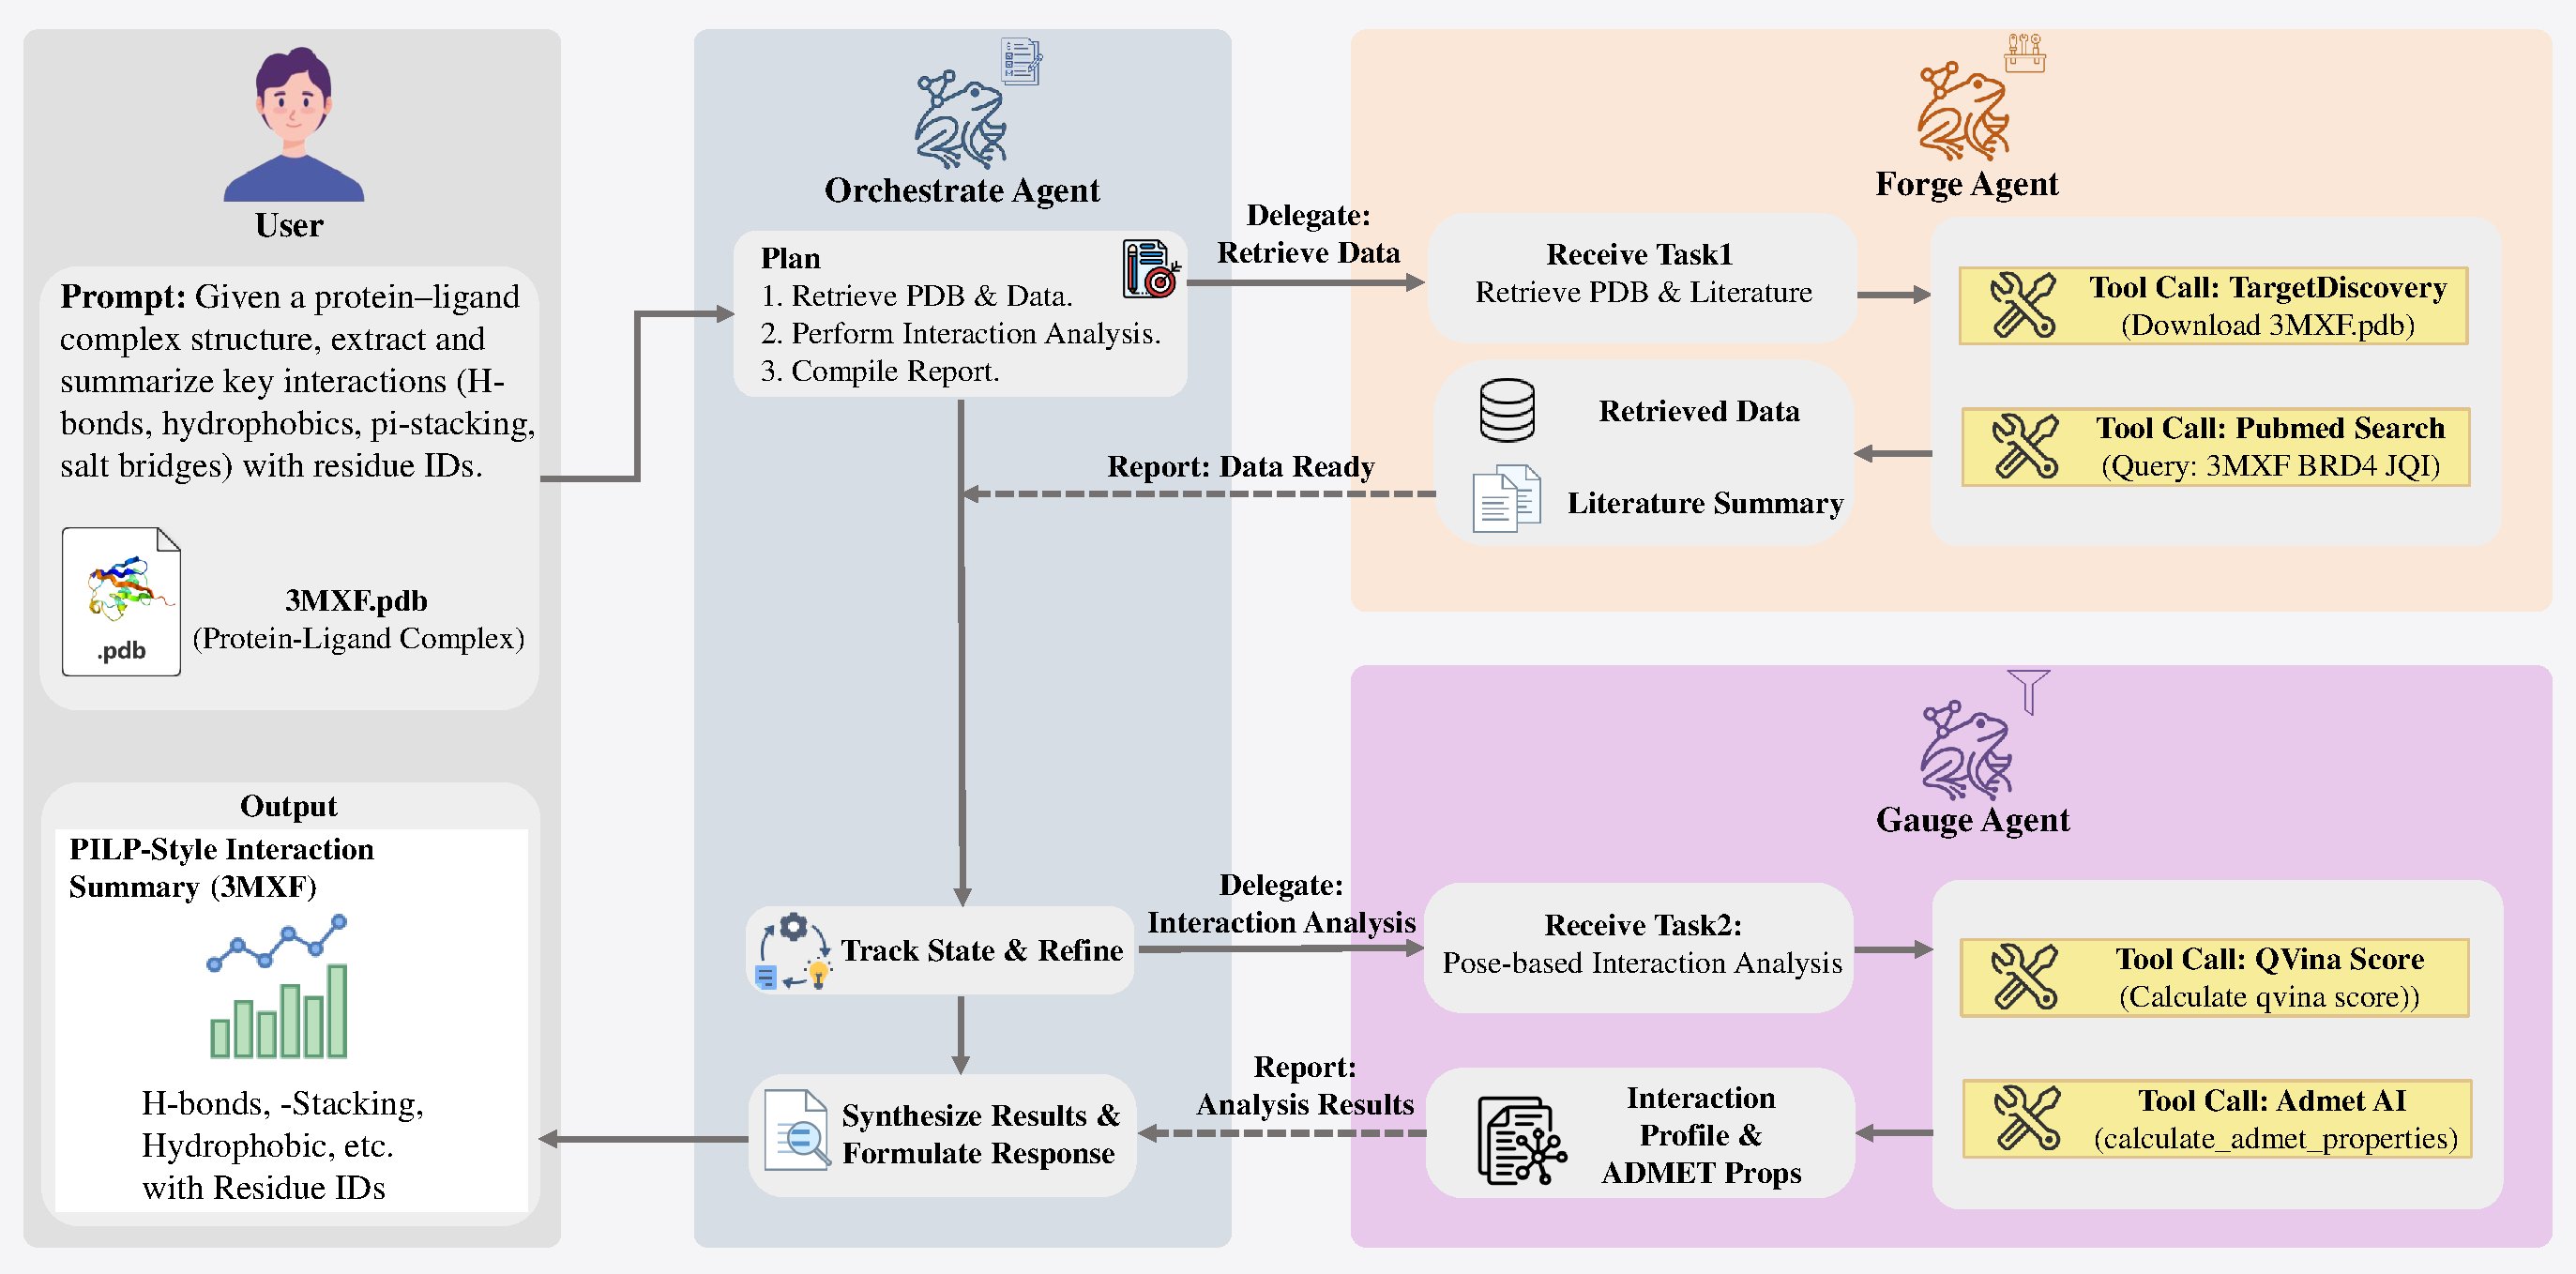
\includegraphics[width=1\textwidth]{figures/frogent-ex7.pdf}
\caption{\textbf{Interaction Analysis Workflow.} A collaborative task where the \oa \ coordinates the \ra \ to gather PDB data and literature provenance, while tasking the \ga \ to perform the quantitative, pose-based interaction analysis before synthesizing a final summary.}
\label{fig:appendix_interaction}
\end{figure*}

\begin{figure*}[!ht]
\centering
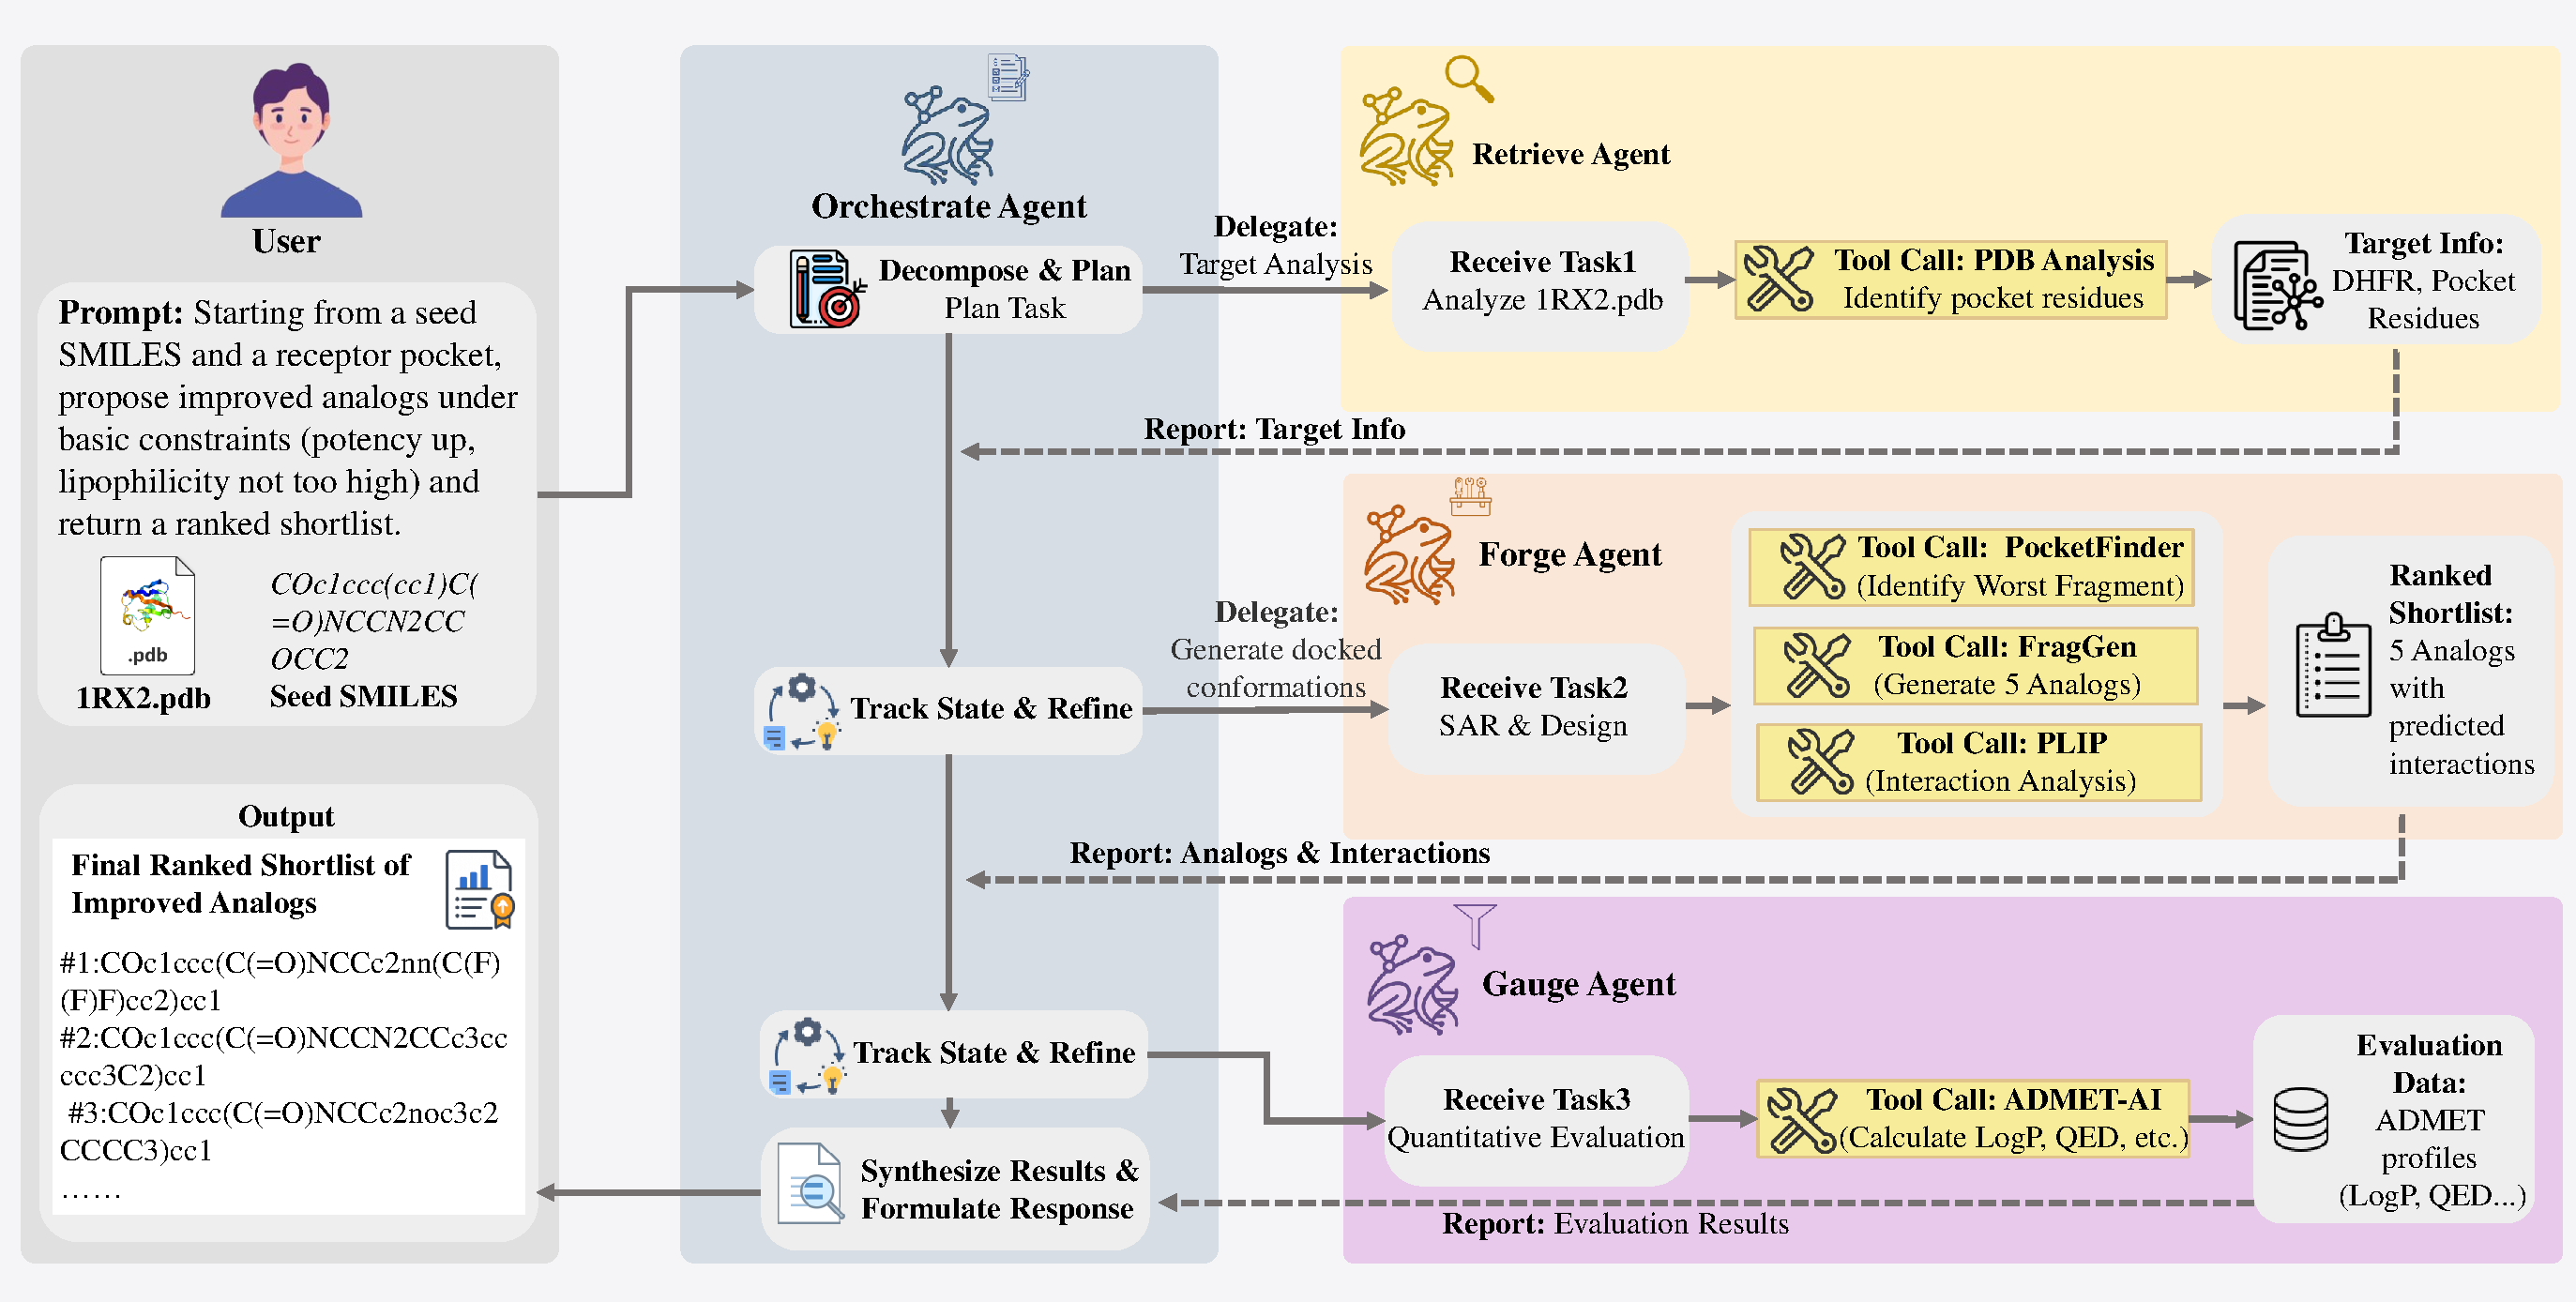
\includegraphics[width=1\textwidth]{figures/frogent-ex8.pdf}
\caption{\textbf{Lead Optimization Workflow.} The core iterative design-evaluate-refine loop of the \name system. The \oa \ supervises the entire process, tasking the \ra \ for initial target analysis, then managing the feedback cycle between the \fa \ (generating improved analogs) and the \ga \ (evaluating them quantitatively).}
\label{fig:appendix_lead_opt}
\end{figure*}

\subsubsection*{Utility and Synthesis Tasks}
\nam's capabilities extend to essential utility tasks and the final stages of a computational campaign. Property prediction is handled as a direct delegation from the \oa \ to the \ga, which executes the task and returns a structured report (Figure~\ref{fig:appendix_property_pred}). The complex task of retrosynthesis planning is managed by the \oa, which tasks the \fa \ to generate and analyze potential synthetic routes using its specialized tools (Figure~\ref{fig:appendix_synthesis}). Finally, the entire discovery process culminates in the report writing workflow (Figure~\ref{fig:appendix_report}). Here, the \oa \ acts as a coordinator and compiler, tasking each specialized agent to contribute its specific data and analysis before synthesizing all components into a single, publication-ready computational drug design report.

\begin{figure*}[!ht]
\centering
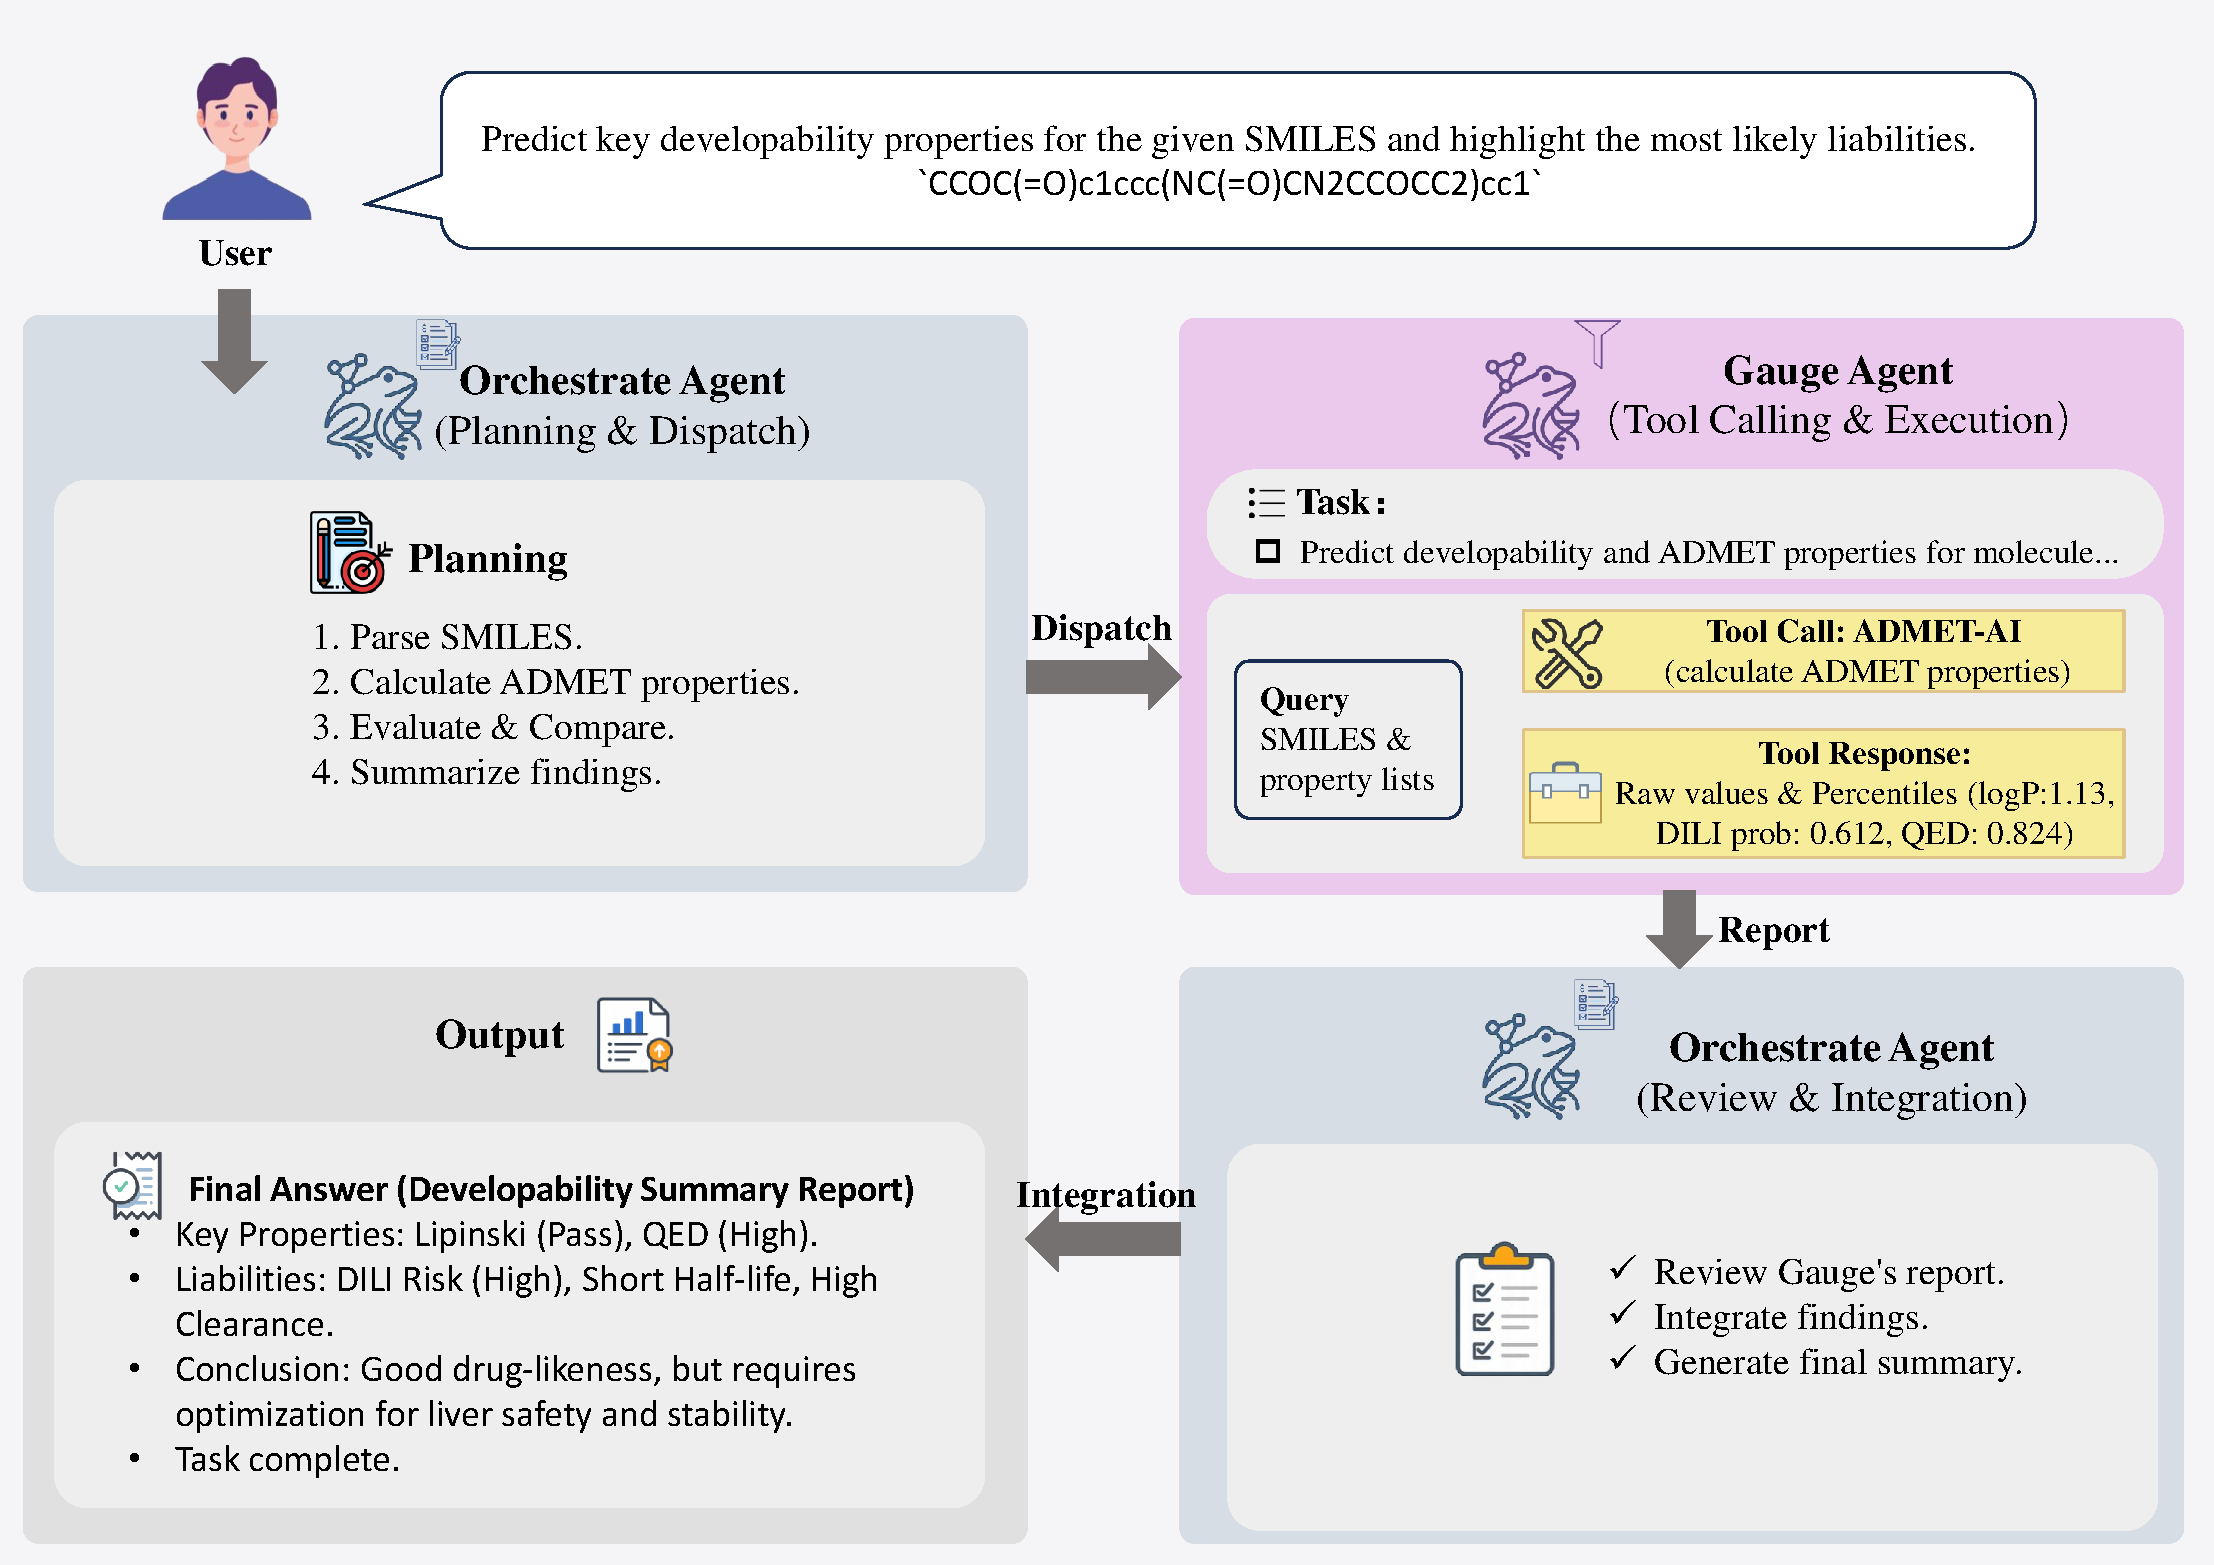
\includegraphics[width=1\textwidth]{figures/frogent-ex9.pdf}
\caption{\textbf{Property Prediction Workflow.} A core utility task showcasing a clear delegation protocol. The \oa \ plans the analysis and tasks the Gauge Agent to execute the ADMET property prediction, which then returns a structured report that the \oa \ integrates into a final summary.}
\label{fig:appendix_property_pred}
\end{figure*}

\begin{figure*}[!ht]
\centering
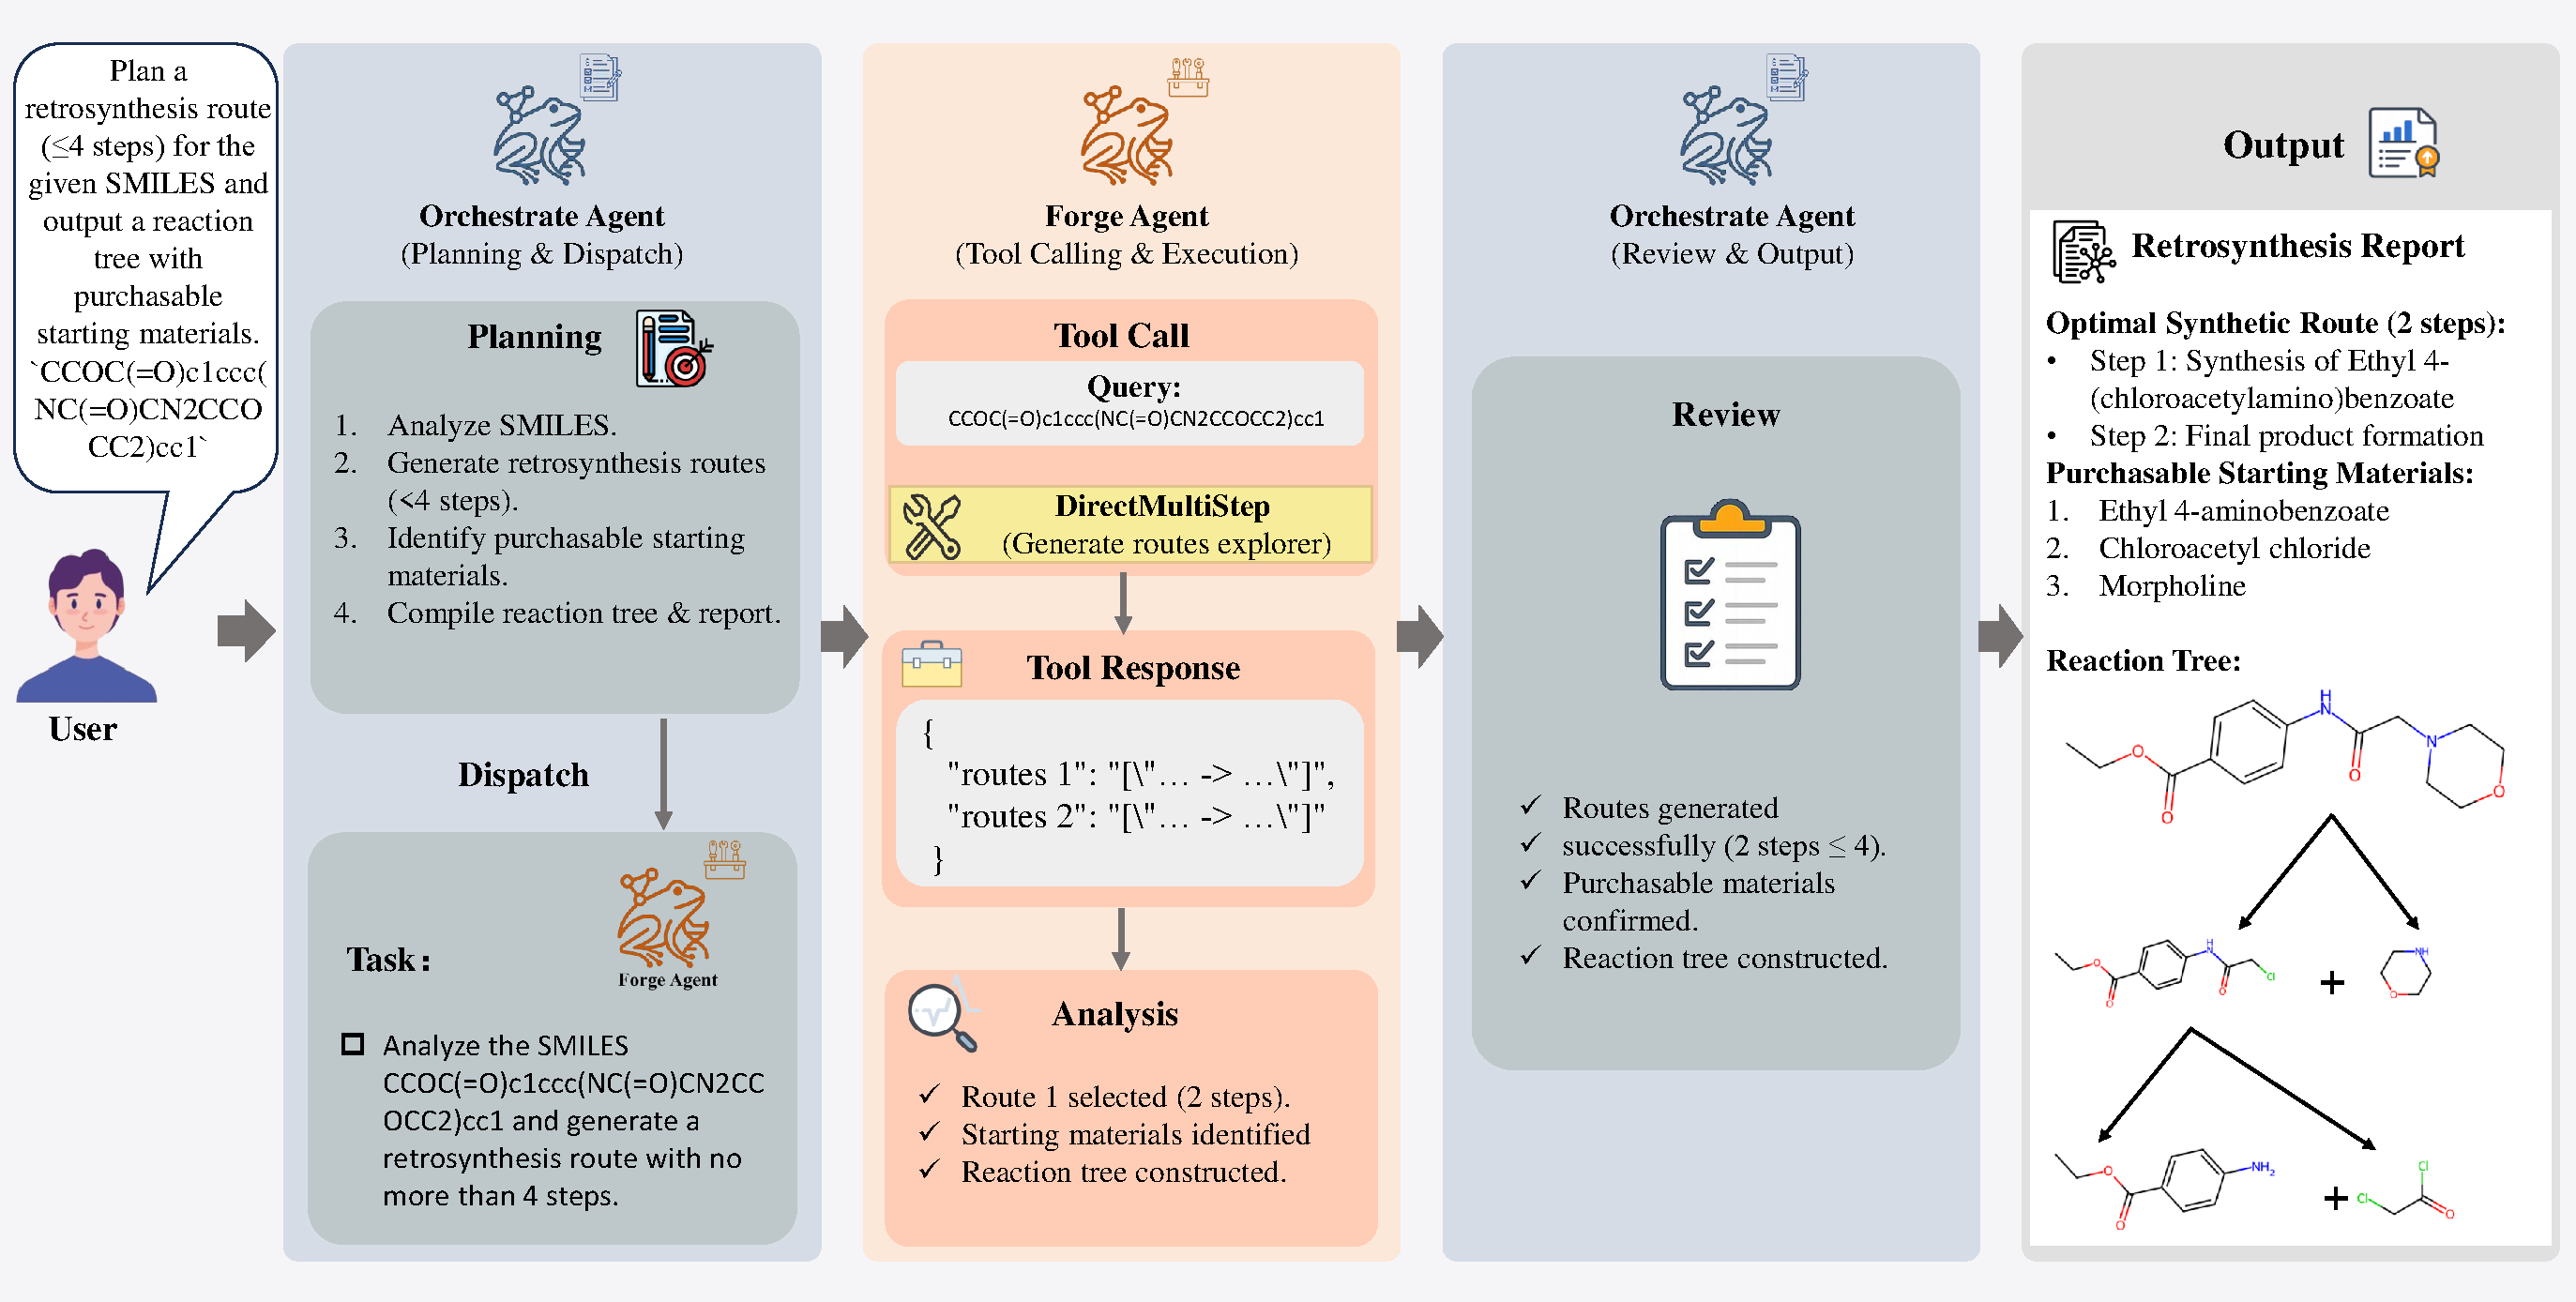
\includegraphics[width=0.96\textwidth]{figures/frogent-ex10.pdf}
\caption{\textbf{Synthesis Planning Workflow.} A complex generative task managed by the \oa. It tasks the \fa \ to generate potential retrosynthesis routes, which analyzes the tool's output to select an optimal pathway and construct a final, structured report including the reaction tree.}
\label{fig:appendix_synthesis}
\end{figure*}

\begin{figure*}[!h]
\centering
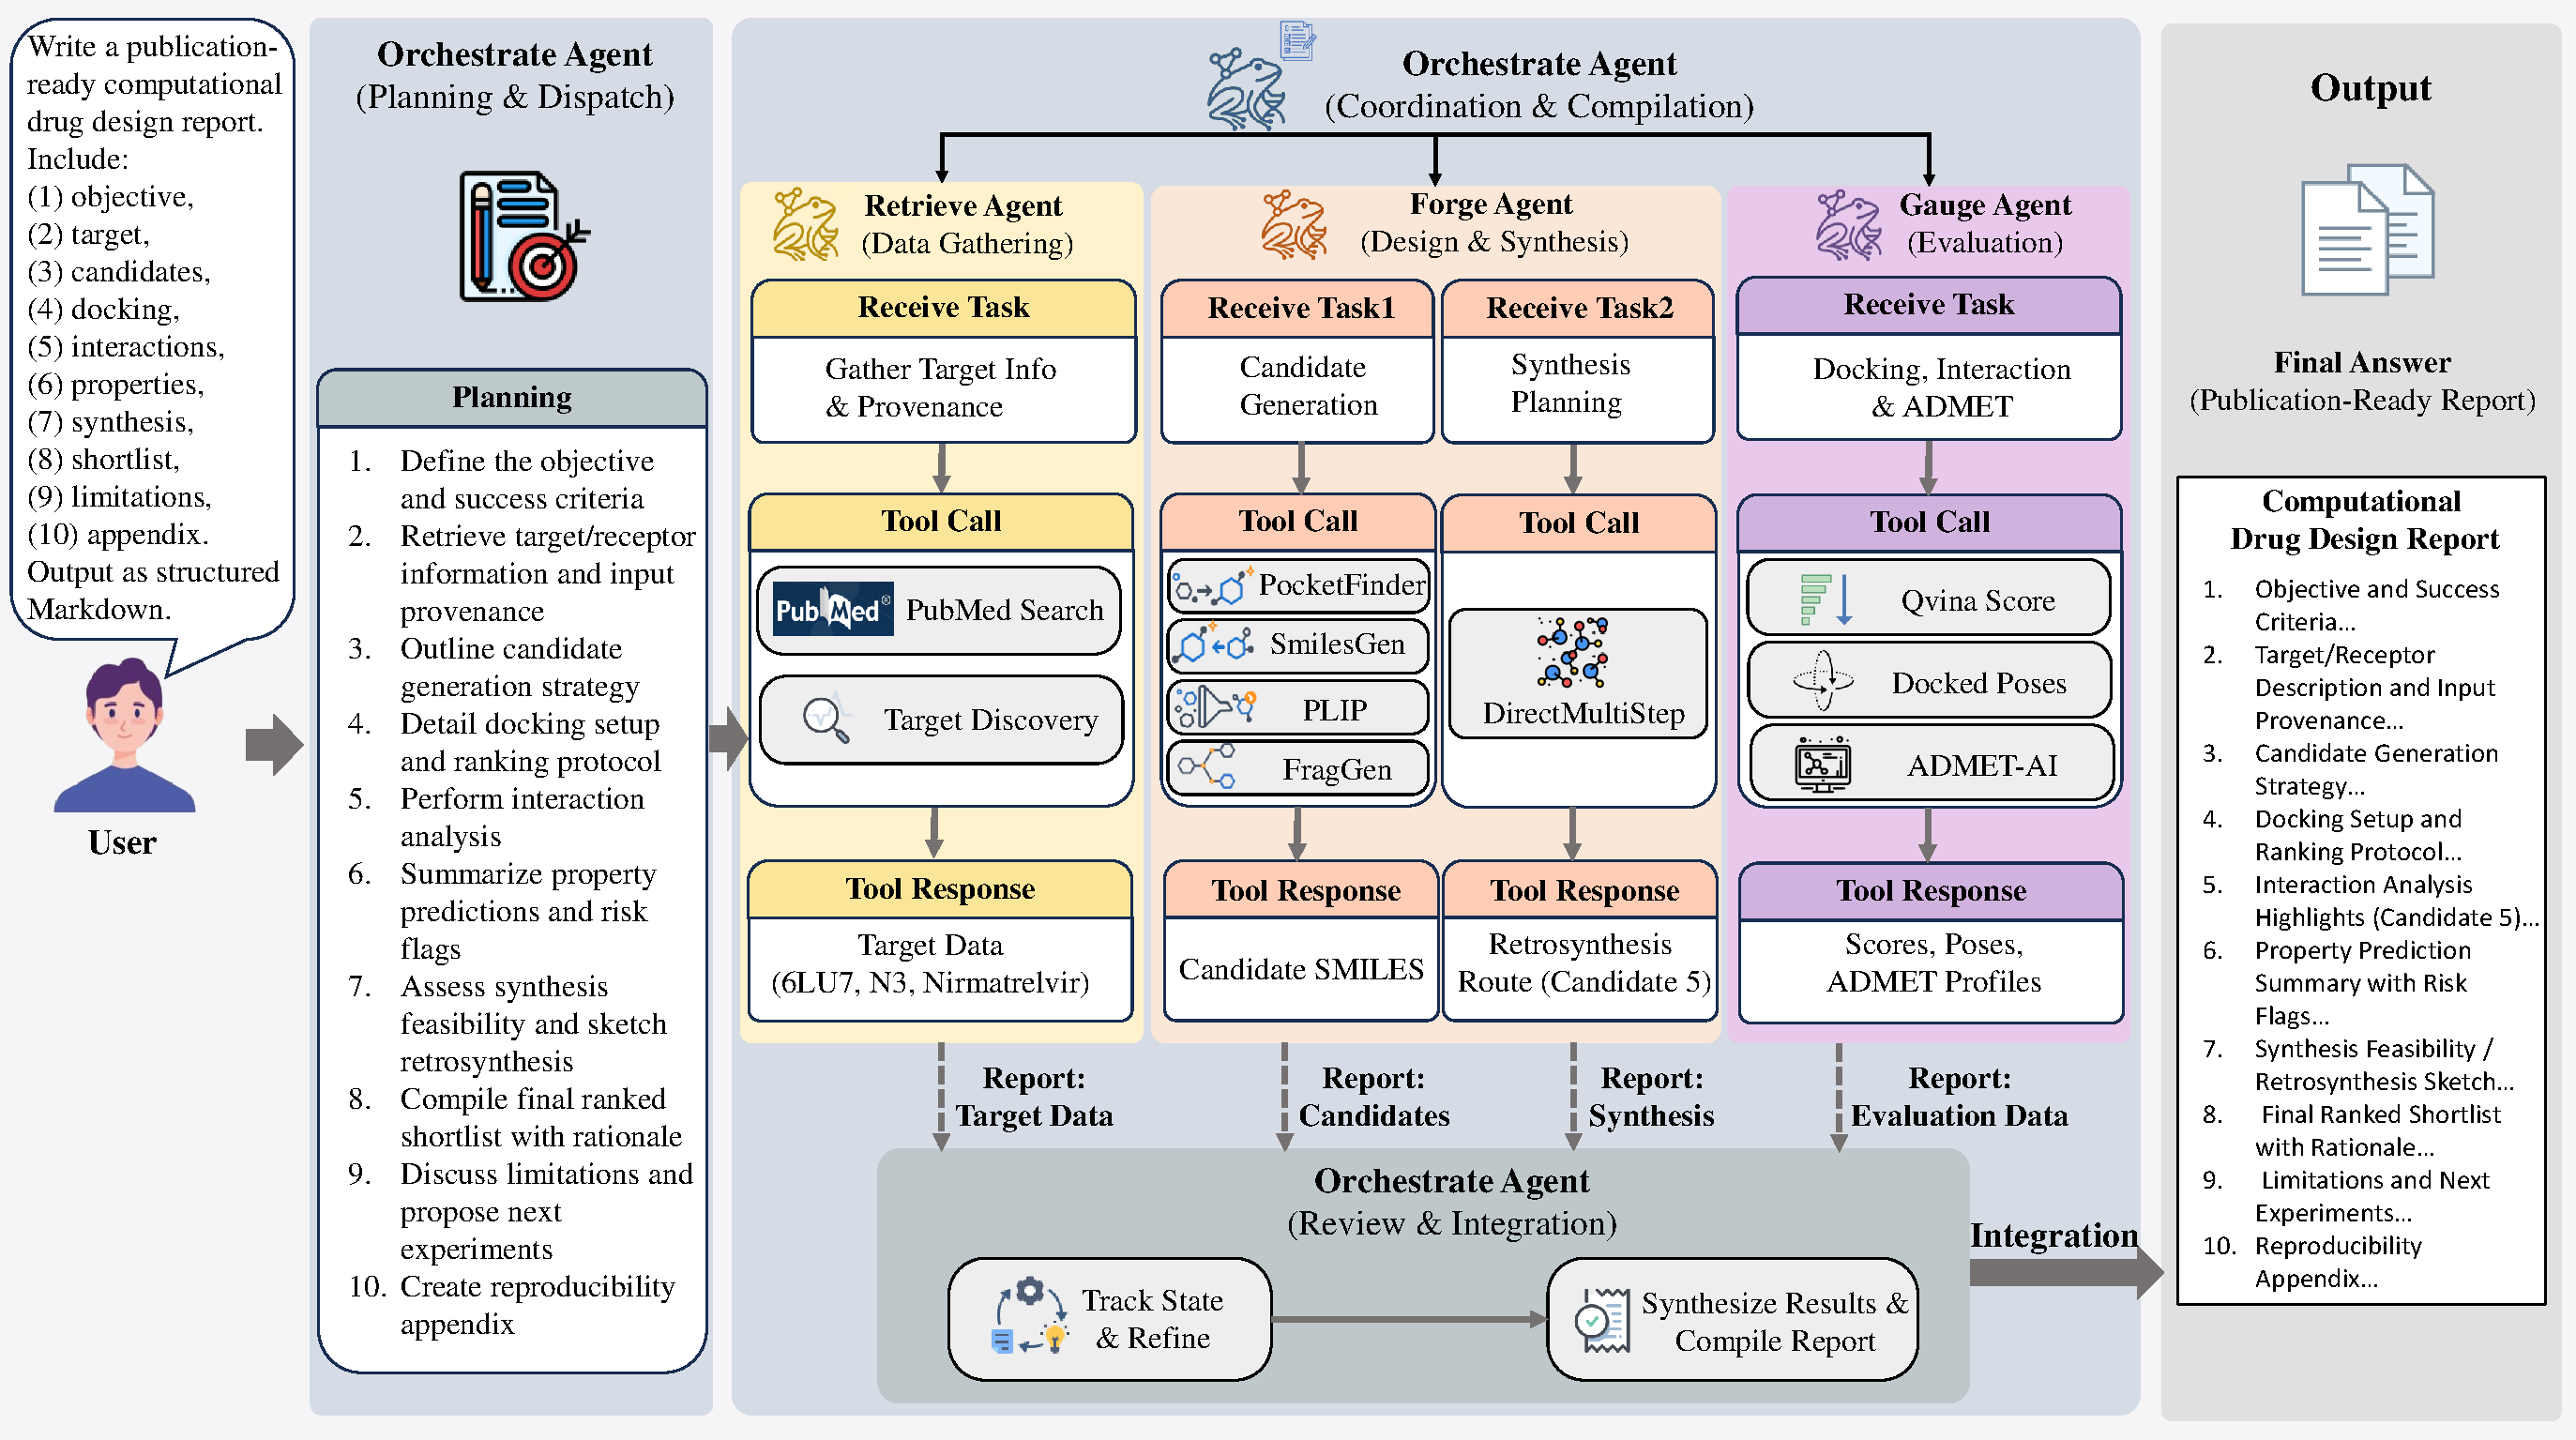
\includegraphics[width=0.96\textwidth]{figures/frogent-ex11.pdf}
\caption{\textbf{Report Writing Workflow.} The final synthesis stage of a discovery campaign. The \oa \ acts as a compiler, dispatching tasks to the \ra, \fa, and \ga \ to gather all necessary data components (e.g., target info, candidate SMILES, evaluation data) before integrating them into a final, publication-ready report.}
\label{fig:appendix_report}
\end{figure*}

%TC:endignore
\section*{Data Availability}
The benchmark inputs and reference records were derived from the public resources identified in the Methods and Supplementary Information, including UniProt, Open Targets, DAVIS, RCSB PDB, CrossDocked, USPTO-50k, and PaRoutes. Versioned evaluation protocols, case definitions, scoring code, aggregate tables, and the manuscript-facing evidence ledger are provided with the public FROGENT repository. Provider-licensed data and third-party model weights are not redistributed. DrugBank-specific live execution was unavailable in the revision environment and is not represented as a measured provider result.

\section*{Code Availability}
FROGENT source code, installation instructions, tests, evaluation entry points, and manuscript assets are available at \url{https://github.com/SZU-ADDG/FROGENT}. The repository excludes credentials, licensed software, model weights, runtime databases, and generated user data. Live workflows require users to configure only the credentials and third-party resources needed by the selected providers; the no-credential core, local application path, and frozen evaluation replay are documented separately.

\section*{Acknowledgements}
This work was supported by the National Natural Science Foundation of China under Grant 6247617, the Guangdong Natural Science Foundation Project under Grant 2025A1515011567, and the Shenzhen Science and Technology Program under Grant JCYJ20220531101614031.

\section*{Declaration of Interests}
The authors declare no competing interests.

\newpage
\nolinenumbers
\bibliography{bibliography}
\bibliographystyle{naturemag}
\end{document}
